\documentclass[ALICE,manyauthors]{ALICE_internal_notes}

\newcommand{\slfrac}[2]{\left.#1\right/#2}
\usepackage{rotating}
%

\usepackage{graphicx}% Include figure files
\usepackage{dcolumn}% Align table columns on decimal point
\usepackage{bm}% bold math
\usepackage{ifpdf}
\usepackage{graphicx}
\usepackage{longtable}
\usepackage{amssymb}
\usepackage{epsfig}
\usepackage{enumerate}
\usepackage{pifont}
\usepackage{hyperref}
\usepackage{verbatim}
\usepackage{lineno}

\usepackage{pslatex}
\usepackage[T1]{fontenc}
\usepackage[latin1]{inputenc}
\usepackage{geometry}

\usepackage{setspace}

\usepackage{listings}

%%configuration de listings
\lstset{
language=c++,
basicstyle=\ttfamily\small, %
identifierstyle=\color{red}, %
keywordstyle=\color{blue}, %
stringstyle=\color{black!60}, %
commentstyle=\it\color{green!95!yellow!1}, %
columns=flexible, %
tabsize=2, %
extendedchars=true, %
showspaces=false, %
showstringspaces=false, %
numbers=left, %
numberstyle=\tiny, %
breaklines=true, %
breakautoindent=true, %
captionpos=b
}

\usepackage{xcolor}

\definecolor{Zgris}{rgb}{0.87,0.85,0.85}

\newsavebox{\BBbox}
\newenvironment{DDbox}[1]{
\begin{lrbox}{\BBbox}\begin{minipage}{\linewidth}}
{\end{minipage}\end{lrbox}\noindent\colorbox{Zgris}{\usebox{\BBbox}} \\
[.5cm]}


\newcommand{\piz}{$\pi^{0}$}
\newcommand{\pip}{$\pi^{+}$}
\newcommand{\pim}{$\pi^{-}$}
\newcommand{\kap}{K$^{+}$}
\newcommand{\kam}{K$^{-}$}
\newcommand{\pbar}{$\rm\overline{p}$}
\newcommand{\Jpsi} {\mbox{J\kern-0.05em /\kern-0.05em$\psi$}\xspace}
\newcommand{\degree}{$^{\rm o}$}
\newcommand{\s}{$\sqrt{s}$}
\newcommand{\sN}{$\sqrt{s_{NN}}$}
\newcommand{\dedx}{d$E$/d$x$}
\newcommand{\pp}{pp}
\newcommand {\mom}    {\mbox{\rm  GeV$\kern-0.15em /\kern-0.12em c$}}
\newcommand {\gmom}   {\mbox{\rm  GeV$\kern-0.15em /\kern-0.12em c$}}
\newcommand {\mass} {\mbox{\rm  GeV$\kern-0.15em /\kern-0.12em c^2$}}

\linenumbers

\begin{document}%
%%%%%%%%%%%%% ptdr definitions %%%%%%%%%%%%%%%%%%%%%
%
%%%%%%%%%%%%%%%  Title page %%%%%%%%%%%%%%%%%%%%%%%%
%
\begin{titlepage}

\title{EMCal Offline Documentation}
\ShortTitle{EMCal documentation}   % appears on right page headers
%
\author{EMCal collaboration}

\author{Email:alice-emcal-offline@cern.ch }
%
%\ShortAuthor{ALICE Internal Note 2012}      % appears on left page headers, do not change
%

\begin{abstract}
This document describes the EMCal, it's offline geometry, the software to run a simulation or reconstruct data, the strategy to control the quality of the data, the trigger code and the analysis format.
\end{abstract}
\end{titlepage}
%
\maketitle
\tableofcontents

\newpage


%-----------------------------------------------------------------------------
\section{Introduction}

% It shows very briefly how can we proceed to execute
%some basic things like the event generation, reconstruction and data
%analysis. For more details on how AliRoot works and how the experimental
%data can be analyzed, I strongly recommend to read the AliRoot primer~\cite{ALIROOT:doc}
%(the present document is not a substitute of the ``AliRoot primer''
%but an introduction for beginners), and also the AliEn pages~\cite{ALIEN:alien}
%or go directly to the code in~\cite{ALIROOT:svn}. 
%For detailed information on the EMCAL code you can go to the EMCAL offline pages (work in progress)~\cite{EMCAL:doc}.

%I will assume that you have already AliRoot and its environment properly
%installed in your machine, if not, look at \cite{ALIROOT:doc} or to the offline installation page \cite{ALIROOT:install}.
%If you type ``cd \$ALICE\_ROOT'', you will find all the AliRoot
%code. In the directories ``\$ALICE\_ROOT/macros'' and ``\$ALICE\_ROOT/EMCAL/macros'', you will find different examples of macros. All the EMCal
%code is in ``\$ALICE\_ROOT/EMCAL'', in case you want to study
%thoroughly how the simulation, reconstruction and analysis software
%code of the calorimeter work. 

%If we want to generate some data (realistic physics data or just single
%particle to study the performance of the ALICE detectors) or read
%real experimental data, and analyze it with AliRoot, we have to pass
%through three steps: \textbf{simulation}, \textbf{reconstruction}
%and \textbf{analysis}. This steps are explained in the next sections. 

This document is addressed to those who want to work with the EMCal data. It explains the different steps to have the data taken ready to be analyzed: geometrical description of the detector, how to get the calibration, how works the simulation and reconstruction of the data and how to access the analysis objects, ESDs and AODs.\\

For introduction on the detectors, the TDR's of the EMCal and DCal can be found in ~\cite{EMCalTDR,DCalTDR}.
For a fast introduction on the code and how it works you can have a look to the EMCal for beginners guide \cite{EMCAL:beginners}. Some other interesting references are the AliRoot primer~\cite{ALIROOT:doc}, the offline AliRoot page \cite{ALIROOT}, and the installation page from Dario Berzano \cite{ALIROOT:berzano}.\\

In general, a lot of information can be found in many twikis collected in the main EMCal twiki page that can be found here~\cite{EMCAL:MainTwiki} and also is interesting to point to the main EMCal offline twiki that can be found here~\cite{EMCAL:OffTwiki}.

\subsection{Mechanical description of the EMCAL}
(Federico Ronchetti)\\

The chosen technology is a layered Pb-scintillator sampling calorimeter with a longitudinal pitch of 1.44 mm Pb and 1.76 mm scintillator with longitudinal 
Wavelength Shifting Fiber (WLS) light collection, see the EMCal TDR~\cite{EMCalTDR}. The full detector spans $\eta$ = -0.7 to $\eta$= 0.7 with an azimuthal acceptance of $\Delta\phi~107^\circ$ 
and is segmented into 12,288 towers, each of which is approximately projective in $\eta$ and $\phi$ to the interaction vertex. 
The towers are grouped into super modules of two types: full size which span $\Delta\phi=20^\circ$ (24 ($\phi$) $\times$48 ($\eta$) towers) and 1/3 size which span $\Delta\phi$ = 6.67$^\circ$  (8 ($\phi$) $\times$48 ($\eta$) towers). 
There are 10 full size and 2, 1/3-size super modules in the full detector acceptance (Fig. \ref{fig:emcal-full}). \\

\begin{figure}[ht]
\begin{center}
\includegraphics[width=1.0\textwidth]{figures/emcal-full.pdf}
\end{center}
\caption{\label{fig:emcal-full} Azimuthal view from the A-side (opposite to the di-muon arm) of the full EMCal as installed into the ALICE detector.
The two 1/3-size super-modules are visible at ~9 o'clock position.}
\end{figure}


In 2014, DCal extension was installed \cite{DCalTDR}, consisting of 6 super modules, with 2/3 the acceptance of an EMCal super-module (same acceptance in $\phi$ smaller in $\eta$ where 0.22$<|\eta|<$0.7,  24($\phi$)$\times$32 ($\eta$) towers) and 2 super-modules with 1/3 acceptance like for the EMCal. This extension covers 67 degrees in azimuth and same coverage in $\eta$ as the EMCal if one considers PHOS, although there is a gap of approx. 0.09 pseudo-rapidity units between PHOS and DCal super-modules, see Fig.~\ref{fig:dcal}. DCal is located opposite to EMCal, in azimuth, in the ALICE coordinate system EMCal is located at 80$<\phi <$187 degrees and DCal at 260$< \phi <$ 327 degrees. The total number of towers in DCal is 5,376.\\


\begin{figure}[ht]
\begin{center}
\includegraphics[width=0.5\textwidth]{figures/DCalPHOS.jpg}
\end{center}
\caption{\label{fig:dcal} Cartoon of the DCal+PHOS configuration in super-modules.}
\end{figure}


The super module is the basic structural units of the calorimeter. 
These are the units handled as the detector is moved below ground and rigged during installation. 
Fig.~\ref{fig:emc-sm} 
%shows a super module with its external mechanical structure stripped away to illustrate the stacking of modules within the super module. 
shows a full size super module with $12\times24$ modules configured as 24 strip modules of 12 modules each. DCal super modules contain $12\times16$ modules, 16 strip modules of 12 modules each.
The supporting mechanical structure of the super module hides the stacking into a nearly projective geometry which can be inferred by the different tilt
of the strip modules from lower $\eta$ to higher $\eta$. %going from the left to the right part of the picture. 
The electronics integration pathways are also visible. 
Each full size super module is assembled from $12 \times 24$ = 288 modules arranged in 24 strip modules of 12 modules each. 

\begin{figure}[ht]
\begin{center}
\includegraphics[width=1.0\textwidth]{figures/emc-sm.jpg}
\end{center}
\caption{\label{fig:emc-sm} View of one EMCal super-module during the installation into the ALICE detector. The cradle holds the 24 strip modules into a mechanically rigid unit.
Each strip module holds 12 unit modules. On the right side the two electronics crates are visible. }
\end{figure}

Each module has a rectangular cross section in the $\phi$ direction and a trapezoidal cross section in the $\eta$ direction with a full taper of 1.5$^\circ$. 
The resultant assembly of stacked strip modules is approximately projective with an average angle of incidence of less than 2$^\circ$ in $\eta$ and 
less than 5$^\circ$ in $\phi$. An assembled strip module is shown in Fig. \ref{fig:strip}.

\begin{figure}[ht]
\begin{center}
\includegraphics[width=0.5\textwidth]{figures/strip-module.pdf}
\end{center}
\caption{\label{fig:strip} View of a fully assembled strip module. The photo shows the APD+CSP package and copper shielding monunted light guide fixture. On the right part
of the photo the LED UV optical fiber distribution system is visible. Each strip module, is cabled via 3 T-Cards visible in the center of the assembly.}
\end{figure}

The smallest building block of the calorimeter is the individual module illustrated in Fig. \ref{fig:module}.
Each individual module contains $2\times 2$ = 4 towers built up from 77 alternating layers of 1.44 mm Pb and 1.76 mm polystyrene, 
injection molded scintillator. White, acid free, bond paper serves as a diffuse reflector on the scintillator 
surfaces while the scintillator edges are treated with TiO2 loaded reflector to provide tower to tower optical 
isolation and improve the transverse optical uniformity within a single tower. 
The Pb-scintillator stack in a module is secured in place by the static friction between individual 
layers under the overall  load of ~350 kg. The module is closed by a skin of 150 $\mu$m thick stainless 
steel screwed by flanges on all four transverse surfaces to corresponding front and rear aluminum  plates. 
This thin stainless skin is the only inert material between the active tower volumes. 
The internal pressure in the module is stabilized against thermal effects, 
mechanical relaxation and long term flow of the Pb and/or polystyrene by a customized 
array of 5 non-linear spring sets (Bellville washers) per module. 
In this way, each module is a self supporting unit with a stable mechanical lifetime of 
more than 20 years when held from its back surface in any orientation as when mounted in a strip module.

%\begin{figure}[ht]
%\begin{center}
%\end{center}
%\caption{\label{fig:module} 
%
%}
%\end{figure}


\begin{figure}[ht]
\begin{center}
\includegraphics[width=0.45\textwidth]{figures/open-module.jpg}
\includegraphics[width=0.32\textwidth]{figures/emc-module.jpg}
\end{center}
\caption{\label{fig:module} The first 1.5$^\circ$ tapered module of the EMCal generation II prototype produced in EU shown: Left: Internal Pb-scintillator sandwich of EMCal modules. Right: The module's internal compression is maintained by a set of 5 Bellville washers (non linear springs) acting between the top and bottom containment 
Al plates to prevent the delamination of the internal Pb-scintillator sandwich.
}
\end{figure}


All modules in the calorimeter are mechanically and dimensionally identical. The front face dimensions of the 
towers are $6\times6$ $cm^2$ resulting in individual tower acceptance of $\Delta\eta\times\Delta\phi=0.014\times0.014$ at $\eta$=0.
The EMCal design incorporates a moderate detector average active 
volume density of ~5.68 g/cm$^3$ which results from a 1:1.22 Pb to scintillator ratio by volume shown in Fig.~\ref{fig:module}. 
This results in a compact detector consistent with the EMCal integration volume at the chosen detector thickness of 20.1 radiation lengths. 
%Practical considerations, including the total assembly labor cost, 
%suggest reducing the total number of Pb/scintillator layers thus decreasing the sampling frequency. 

As described above, the super module is the basic building block of the calorimeter. 
Starting with 288 individual modules which are rather compact and heavy, the main engineering task is to create a super module structure which is rigid, 
with small deflections in any orientation yet does not require extensive, heavy external stiffening components that would reduce the volume available for the active detector. 
The solution adopted for the ALICE EMCal is to develop a super module crate which functions not as a box for the individual modules 
but rather an integrated structure in which the individual elements contribute to the overall stiffness. 
The super module crate is effectively a large I-beam in which the flanges are the long sides of the crate and the 24 rows of strip modules together. 
This configuration gives to the super module good stiffness for both the 9 o'clock and 10 o'clock locations. For the 12 o'clock location, 
the I-beam structure of the super module is augmented by a 1 mm thick stainless steel forward sheet (traction loaded), 
which controls the bending moment tending to open the crate main sides, and helps to limit deflection of strip modules. 
Ridges are provided on the interior surfaces of the crate to allow precision alignment of the strip modules at the correct angle. 
The stiffness given by this I-beam concept allows the use of non-magnetic light alloys for main parts of the super module crate. 
Parts of the super module crate will be made mainly from laminated 2024 aluminum alloy plates. 
The two main sides (flanges of the I-beam) of the crate will be assembled from 2 plates, 25 mm and 25 mm thick, 
bolted together and arranged so as to approximately follow the taper of the 20 degree sector boundary. Each of the 24 rows of a super module contain 12 modules as described above. 
Each of the modules is attached to a transverse beam by 3.4 mm diameter stainless steel screws. 
The 12 modules and the transverse beam form a strip module. The strip module is 1440 mm long, 120 mm wide, 410 mm thick. 
The total weight of the strip module is approximately 300 kg and like module, it is a self supporting unit. 
The transverse beam, which is the structural part of the strip module, is made from cast aluminum alloy 
with individual cavities along its length where the fibers emerging from towers are allowed to converge. 
The casting process is well suited to forming these cavities and the overall structure, saving considerable raw material and machining time. 

In addition to functioning as a convenient structural unit which offers no interference with the active volume of the detector 
and forming the web of the I-beam structure of the super module, the transverse beam of the strip module provides protection for the fibers, 
a structural mount for the light guide, APD and charge sensitive preamplifier and a light tight enclosure for these elements.


\subsection{Functional description of the EMCAL}

%**** need some additional info on PE APDs *********
%EMCAL basic units are cells/towers (Pb-scintillator sandwich of about 70 layers). We have 12 SuperModules (4 in 2010, 10 in 2011-2012) composed of 24 (phi direction) x 48 (eta direction) cells (except last 2 SuperModules made of 8 cells in phi direction). 

Particles traversing the calorimeter, in particular photons and electrons, will deposit energy in different towers. 
The EMCAL reconstruction measures such energy per tower, forms clusters of cells produced by a given particle, 
and if possible matches them with particles detected by the tracking detectors in front of EMCAL (charged particles).

Scintillation photons produced in each tower are captured by an array of 36 Kuraray, 
Y-11, double clad, WLS fibers that run longitudinally through the Pb/scintillator stack.
Each fiber terminates in an aluminized mirror at the front face end of the module and is integrated into a polished, 
circular group of 36 at the photo sensor end at the back of the module. 
The fiber bundles are pre-fabricated and inserted into the towers after the module mechanical assembly is completed. 
The 36 individual fibers are packed into a circular array 6.8 mm in diameter and held in place inside a custom injection 
molded grommet by Bicron BC-600 optical cement. An optical quality finish is applied to the assembled bundle using a diamond polishing machine. 
At the other end of the bundle, individual fibers are similarly polished and mirrored with a sputtered coat 
of aluminum thick enough to ensure the protection of the inner mirror. 
The response of the Al-coated fiber is considerably flatter with an overall increase in efficiency in the range of about 25\% in the vicinity of shower maximum 
(i.e. the location of the highest energy deposition for an electromagnetic shower).  
This number accounts for material immediately in front of the detector; which ranges between 0.4 and 0.8 radiation lengths, 
and assumes 5.5 - 6.0 radiation lengths for shower maximum for 10 GeV photons. 
At this depth in the detector, the mirrored fiber response is very uniform does not contribute to the non-linearity of the detector as a whole. 

Other factors which can significantly impact the electromagnetic performance of the calorimeter, 
include scintillator edge treatment and the density of the wavelength shifting fiber readout pattern and the material 
chosen for the interlayer diffuse reflector. For scintillator edge treatment and fiber density, advantage was taken from the 
extensive studies made by the LHCb collaboration for their ECAL. In particular, a diffuse reflector edge treatment was adopted, 
such as that obtained with Bicron Titanium Dioxide loaded white paint (BC622A) with a total fiber density of about one fiber per $cm^2$. 
In the case of the interlayer diffuse reflector, a white, acid free, bond paper was used in place of the Teflon based commercial TYVEK. 
While TYVEK produces slightly better surface reflectivity, its coefficient of friction is too low to permit its use in this 
design where the module's mechanical stability depends somewhat on the interlayer friction.
 
The 6.8 mm diameter fiber bundle from a given tower connects to the APD through a short light guide/diffuser 
with a square cross section of 7 mm $\times$ 7 mm that tapers slowly down to 4.5 mm $\times$ 4.5 mm as it mates (glued) 
to the 5 mm $\times$ 5 mm active area of the photo sensor. 
The 4 pre-fabricated fiber bundles are inserted into the 
towers of a single module. 

The selected photo sensor is the Hamamatsu S8664-55 Avalanche Photo Diode.
% ************
This photodiode has a peak spectral response at a wavelength of 585 nm compared to an emission peak of 476 nm for the Y-11 fibers. 
However, both the spectral response and the quantum efficiency of the APD are quite broad with the latter dropping from the maximum by only ~5\% at the WLS fiber emission peak. 
At this wavelength, the manufacturer's specification gives a quantum efficiency of 80\%. 

\newpage

\section{EMCAL geometry software}
(Marco Bregant, Alexandre Shabetai, Gustavo Conesa Balbastre)\\

This page is intended for a description of the EMCAL geometry and the methods to access it.  
{\it This is a very preliminary version that needs work.}

 \subsection {Classes description}

The EMCAL geometry is implemented in several classes : {\color{red} (right now very brief description, it should be completed) }
\begin{itemize}
\item AliEMCALGeometry: Steering geometry class.  No dependencies on STEER or EMCAL non geometry classes. Can be called during the analysis without loading all AliRoot classes.
\item AliEMCALEMCGeometry: Does the geometry initialization. Does all the definitions of the geometry (towers composition, size, Super Modules number ...)
\item AliEMCALGeoParams:  Class container of some of the geometry parameters so that it can be accessed everywhere in the EMCAL code, to avoid "magic numbers". Its use has to be propagated to all the code.
\item AliEMCALShishKebabTrd1Module: Here the modules are defined and the position of the modules in the local super module reference system is calculated
\end{itemize}

\subsection{Accessing the geometry}
One can get the geometry pointer in the following way:

%\begin{DDbox}{\linewidth}
\begin{lstlisting}
AliEMCALGeometry * geom =  AliEMCALGeometry::GetInstance(GeoName) ;
\end{lstlisting}
%\end{DDbox}

where "GeoName" is a string, the different options are specified in the next section. If you have a already generated simulation file and want to access the geometry used there, if the file {\it galice.root} is available:

\begin{DDbox}{\linewidth}
\begin{lstlisting}
AliRunLoader *rl = AliRunLoader::Open("galice.root",AliConfig::GetDefaultEventFolderName(),"read"); 
rl->LoadgAlice();//Needed to get geometry
AliEMCALLoader *emcalLoader = dynamic_cast<AliEMCALLoader*>(rl->GetDetectorLoader("EMCAL"));
AliRun * alirun = rl->GetAliRun();
AliEMCAL * emcal = (AliEMCAL*)alirun->GetDetector("EMCAL"); AliEMCALGeometry * geom = emcal->GetGeometry();
\end{lstlisting}
\end{DDbox}

In this case you might need the file {\it geometry.root} if you want to access to certain methods that require local to global position transformations. This file can be generated doing a simple simulation, it just contains the transformation matrix to go from global to local.

The way to load this file is:
%\begin{DDbox}{\linewidth}
\begin{lstlisting}
TGeoManager::Import("geometry.root");
\end{lstlisting}
%\end{DDbox}

The transformation matrices are also stored in the ESDs so if you do not load this file, you can have to load these matrices from the ESDs. They are also stored in the OADB.

 If you want to see different parameters used in the geometry printed (cells centers, distance to IP, etc), one just has to execute the method {\it PrintGeometry()}.
 
\subsection{Geometry configuration options}
Right now the following geometry options are implemented:
\begin{itemize}
\item EMCAL\_FIRSTYEARV1: 4 Super Modules, geometry  configuration for year 2010.
\item EMCAL\_COMPLETEV1: 10 Super Modules, geometry configuration for year 2011.
\item EMCAL\_COMPLETE12SMV1: 12 Super Modules (10+2$\times$1/3) full EMCal. Configuration for year 2012, although the 1/3 super-modules where not active.
\item EMCAL\_COMPLETE12SMV1\_DCAL: Full EMCal plus 6 DCal super-modules.
\item EMCAL\_COMPLETE12SMV1\_DCAL\_8SM: Full EMCal plus 6 DCal super-modules plus 2$\times$1/3 EMCal, geometry configuration for Run2 (years 2015-18).
\item EMCAL\_COMPLETE12SMV1\_DCAL\_DEV: Full EMCal plus  10 DCal super-modules (possible future configuration).
\end{itemize}

Other options exists but need to be removed as they {\bf should not be used} or that should be avoided:
\begin{itemize}
\item EMCAL\_PDC06: Old geometry, for reading old data (which do not exist anymore).
\item EMCAL\_WSU: Prototype geometry. 
\item EMCAL\_COMPLETE: 12 Super Modules (2 half Super Modules). Not correct geometry, use "V1" in name
\item EMCAL\_FIRSTYEAR: 4 Super Modules (year 2010). Not correct geometry, use "V1" in name.
\end{itemize}

By default, the geometry is loaded with the EMCAL\_COMPLETE12SMV1 configuration. For details on the implementation of the DCal geometry have a look here~\cite{DCalGeoOff}
 
 \subsection{Setting the geometry in simulations}

When configuring a simulation, a typical file {\it Config.C} is used. Inside this file, the detectors to be used in the generation are specified, and particularly EMCal is initialized in this way:

\begin{lstlisting}
AliEMCAL *EMCAL =  = new AliEMCALv2("EMCAL", TString GeoName, Bool_t checkGeoRun);
\end{lstlisting}

Where:
\begin{itemize}
  \item {\it AliEMCAL} is the main steering class for the simulation. The derived classes {\t AliEMCALvX}:
    \begin{itemize}
    \item {\it AliEMCALv0} does the geometry initialization, materials creation etc.
    \item {\it AliEMCALv1} derives from {\it v0}, DO NOT USE for simulation, originally it was meant for fast simulations, it does not generate hits.
    \item {\it AliEMCALv2} derives from {\it v1}, USE for simulation. It does all the particle propagation in the EMCal material
\end{itemize}
  \item {\it TString GeoName}: Geometry names listed in the previous section
  \item {\it Bool\_t checkGeoRun}: Bool that activates the geometry initialization depending on the run number. Since EMCal geometry changed over time, to avoid mistakes in the configuration files of simulations anchored to particular run numbers,  by default this is set to TRUE and the name set in the initialization of AliEMCAL is not taken into account but the one corresponding to this run.
\end{itemize}

 
 \subsection{Mapping}
The tower row/column mapping online and offline follows the alice numbering convention. Figures~\ref{fig:Map1} to \ref{fig:Map2} display the position of the super modules from different points of view and the position of the tower index in them.

\begin{figure}[ht]
\begin{center}
\includegraphics[width=1.0\textwidth]{figures/EMCALMap0_0.pdf}
\end{center}
\caption{\label{fig:Map1}Position of the super modules}
\end{figure}

\begin{figure}[ht]
\begin{center}
\includegraphics[width=1.0\textwidth]{figures/EMCALMap1.pdf}
\end{center}
\caption{\label{fig:Map0}EMCal seen from the magnet side with 4 SMs.}
\end{figure}


\begin{figure}[ht]
\begin{center}
\includegraphics[width=1.0\textwidth]{figures/EMCALMap2.pdf}
\end{center}
\caption{\label{fig:Map2}EMCal geometrical numbering.}
\end{figure}


\subsection{Tower index transformation methods}
\subsubsection{Absolute tower ID to Row/Column index}

Each EMCAL supermodule is composed of 24x48 towers (phi,eta), grouped in 4x4 modules. Each tower (even each module) has a unique number assigned, called in the code "absolute ID" number (absId). This number can be transformed into a row (phi direction) or column (eta direction) index. The procedure to go from the absId to the (row, col) formulation or viceversa is as follow:

\begin{itemize}
\item From absId to col-row: 

\begin{DDbox}{\linewidth}
\begin{lstlisting}
Int_t nSupMod, nModule, nIphi, nIeta, iphi, ieta;
//Check if this absId exists
if(!CheckAbsCellId(absId)) return kFALSE;
// Get from the absId the super module number, the module number and the eta-phi index (0 or 1) in the module
GetCellIndex(absId, nSupMod, nModule, nIphi, nIeta);
// Get from the  the super module number, the module number and the eta-phi index (0 or 1) in the module the tower row (iphi) and column (ieta) 
GetCellPhiEtaIndexInSModule(nSupMod,nModule,nIphi,nIeta, iphi, ieta); 
\end{lstlisting}
\end{DDbox}

\item From col-row to absId, following the same notation as above: 

\begin{DDbox}{\linewidth}
\begin{lstlisting}

absid = GetAbsCellIdFromCellIndexes(nSupMode, iphi, ieta);
\end{lstlisting}
\end{DDbox}

or

\begin{DDbox}{\linewidth}
\begin{lstlisting}

absid = GetAbsCellId(nSupMod, nModule, nIphi, nIeta);
\end{lstlisting}
\end{DDbox}

\item Other interesting method is

\begin{DDbox}{\linewidth}
\begin{lstlisting}

Int_t   GetSuperModuleNumber(Int_t absId)  
\end{lstlisting}
\end{DDbox}
\end{itemize}

\subsection{Tower index to local / global reference system position}
\subsubsection{Local coordinates}

To correlate the tower index and its position in local coordinates, the following methods are available:

\begin{DDbox}{\linewidth}
\begin{lstlisting}
  Bool_t  AliEMCALGeoUtils::RelPosCellInSModule(Int_t absId, Double_t &xr, Double_t &yr, Double_t &zr) const;

  Bool_t  AliEMCALGeoUtils::RelPosCellInSModule(Int_t absId, Double_t loc[3]) const;

  Bool_t  AliEMCALGeoUtils::RelPosCellInSModule(Int_t absId, TVector3 &vloc) const;
\end{lstlisting}
\end{DDbox}

To which the input is the absId and the output are the coordinates of the center of towers in the local coordinates of the Super Module. This method gets the column and row index of the cell from the absId, independently of the Super Module (like above), and gets the center of the cell from 3 arrays (x,y,z) filled with such quantities. Such central positions are calculated during the initialization of the geometry, where the arrys are filled, in the method :

\begin{DDbox}{\linewidth}
\begin{lstlisting}

  AliEMCALGeoUtils::CreateListOfTrd1Modules()
\end{lstlisting}
\end{DDbox}

{\color{red}<<<<<Someone else should explain how it works>>>>>}

 

In case we calculate the cluster position, things are a bit different.

 

{\color{red}<<<<< This explanation should go to the clusterization section>>>>}

 

This is done in 

\begin{DDbox}{\linewidth}
\begin{lstlisting}
void AliEMCALRecPoint::EvalLocalPosition()
\end{lstlisting}
\end{DDbox}

First we calculate the cell position with the  method 

\begin{DDbox}{\linewidth}
\begin{lstlisting}
AliEMCALGeometry::RelPosCellInSModule(Int_t absId, Int_t maxAbsId, Double_t tmax, Double_t &xr, Double_t &yr, Double_t &zr)
\end{lstlisting}
\end{DDbox}

The calculation of the cell position done here is different in the "x-z" but the same in "y". 

 

{\color{red}<<<<< <<<<<Someone else should explain how it works>>>>>}

 
 

In this particular case the position calculation per tower depends on the position of the maximum cell, and the sum of the energy of the cells of the cluster. The maximum depth (tmax) is calculated with the method

\begin{DDbox}{\linewidth}
\begin{lstlisting}
  Double\t AliEMCALRecPoint::TmaxInCm(const Double_t e){

      //e: energy sum of cells

static Double_t ca = 4.82;// shower max parameter - first guess; ca=TMath::Log(1000./8.07)

      static Double_t x0 = 1.23; // radiation lenght (cm)

      static Double_t tmax = 0.; // position of electromagnetic shower max in cm

      tmax = TMath::Log(e) + ca+0.5;

      tmax *= x0; // convert to cm

  }
\end{lstlisting}
\end{DDbox}

After the cells position of the cluster is accessed, the position of the cluster is calculated averaging the cell positions with a logarithmic weight:

\begin{DDbox}{\linewidth}
\begin{lstlisting}
  w(cell i) = TMath::Max( 0., logWeight + TMath::Log( energy[cell i] / summed_cluster_cell_energy ));
\end{lstlisting}
\end{DDbox}

where the logWeight was chosen to be 4.5 (this value was taken from PHOS, never optimized as far as I know)

So in the end the position,  is 

\begin{DDbox}{\linewidth}
\begin{lstlisting}
f = Sum(f(i) * w(i))/Sum(w(i))
\end{lstlisting}
\end{DDbox}

where f=x,y,z.

 

 \subsubsection{Global coordinates}
 

To transform from local to global we have the methods

\begin{DDbox}{\linewidth}
\begin{lstlisting}

  void GetGlobal(const Double_t *loc, Double_t *glob, int ind) const;

  void GetGlobal(const TVector3 &vloc, TVector3 &vglob, int ind) const;

  void GetGlobal(Int_t absId, Double_t glob[3]) const;

  void GetGlobal(Int_t absId, TVector3 &vglob) const;
\end{lstlisting}
\end{DDbox}

 

 These methods take the local coordinates and transform them into global coordinates using the transformation matrix of the Super Module.

\begin{DDbox}{\linewidth}
\begin{lstlisting}
 

TGeoHMatrix* m = GetMatrixForSuperModule(nSupMod);

if(m) m->LocalToMaster(loc, glob);

\end{lstlisting}
\end{DDbox}
 

 GetGlobal is called in the following useful methods in the geometry class:

 
\begin{itemize}
\item Return the eta and phi angular position of the cell from the AbsId

\begin{DDbox}{\linewidth}
\begin{lstlisting}
void    EtaPhiFromIndex(Int_t absId, Double_t &eta, Double_t &phi) const;
void    EtaPhiFromIndex(Int_t absId, Float_t &eta, Float_t &phi) const;
\end{lstlisting}
\end{DDbox}
\item Print information of the cells. For "pri>0" returns more information. "tit" has not much use, this value is printed.

\begin{DDbox}{\linewidth}
\begin{lstlisting}
void PrintCellIndexes(Int_t absId, int pri, const char *tit)
\end{lstlisting}
\end{DDbox}
\end{itemize} 

\subsection{Geometry Alignment}
AliRoot contains a frame for the correction of the misplacement of geometry objects with respect to the ideal positions which are kept in the STEER/ directory of the following classes:

\begin{DDbox}{\linewidth}
\begin{lstlisting}
AliAlignObj  
AliAlignObjMatrix  
AliAlignObjParams  
AliAlignmentTracks
\end{lstlisting}
\end{DDbox}

The class AliEMCALSurvey creates the corrections to the alignable objects.  The class AliEMCALSurvey was established to take the survey parameters from OCDB, calculate the shift in position of the center of the end faces of the supermodules from the nominal position, and convert this to a transformation matrix for each supermodule which is applied to correct the global position of the supermodules.  All calculations of global positions would then use these corrected supermodule positions to determine their locations within the ALICE global coordinate system. 

\clearpage


\section{EMCal OCDB/OADB - Marcel}

OCDB is the Offline data base. It contains the different parameters used for simulation or reconstruction of the detectors or even the LHC machine parameters that might change for the different run conditions.

OADB is the Offline Analysis data base.

The EMCAL OCDB (and other detectors OCDB) is divided in 3 directories that can be found in 
\begin{lstlisting}
$ALICE_ROOT/OCDB/EMCAL
\end{lstlisting}
\begin{itemize}
\item Calib: Very different type of information, from hardware mapping to calibration parameters. 
\item Align: Survey misplacements in geometry.
\item Config: Detector configuration, temperatures
\end{itemize}

Inside these directories you will find other subdirectories with more specific types of parameters. Each of the directories contains a file named in this way:
\begin{lstlisting}
Run(FirstRun)_(LastRun)_v(version)_s(version).root
\end{lstlisting}
being the default and what you will find in the trunk
\begin{lstlisting}
Run0_999999999_v0_s0.root
\end{lstlisting}

What is actually used for the real data reconstruction can be found in alien here:
\begin{lstlisting}
/alice/data/20XX/OCDB/EMCAL
\end{lstlisting}
There are different repositories for different years (20XX). For the simulation productions, there is another repository on the grid:
\begin{lstlisting}
/alice/simulation/2008/v4-15-Release/XXX/EMCAL
\end{lstlisting}
which is divided into 3 other repositories: Ideal, Full and Residual. Each one is meant to reproduce the detector with different precision. For EMCAL, right now these 3 repositories contain the same parameters.

The following section explain the elements stored and how to read and fill OCDB parameters.

\subsection{Accessing a different OCDB}

In the simulation/reconstruction macro a default OCDB needs to be specified if different from 
\begin{lstlisting} 
$ALICE_ROOT/OCDB.
\end{lstlisting} 
When running on the grid, one needs to set for example in a reconstruction of simulated data:
\begin{lstlisting}
 reco.SetDefaultStorage("alien://Folder=/alice/simulation/2008/v4-15-Release/Residual/");
\end{lstlisting}
If one or several OCDB files have been modified, the following line has to be added in the simulation or reconstruction macro:
\begin{lstlisting}
 reco.SetSpecificStorage("EMCAL/Calib/Pedestals","local://your/modified/local/OCDB");
\end{lstlisting}

The file with the calibration coefficients needs to be stored in the directory :
\begin{lstlisting}
 /your/modified/local/OCDB/EMCAL/Calib/Data 
 \end{lstlisting}
 
If more of the OCDB files are modified, add the following line :
\begin{lstlisting}
 reco.SetSpecificStorage("EMCAL/Calib/","local:/your/modified/local/OCDB");
 \end{lstlisting}
with all the directories inside \begin{lstlisting} EMCAL/Calib \end{lstlisting} and corresponding files put in 
\begin{lstlisting}
/your/modified/local/OCDB/EMCAL/Calib/
\end{lstlisting}

\subsection{Energy calibration}

Calibration Coefficients tower by towers are stored in the following directory :
\begin{lstlisting}
EMCAL/Calib/Data
\end{lstlisting}
What is stored is an object of the class AliEMCALCalibData which is a container of gains and pedestals per tower. These coefficients are used in:
\begin{itemize}
\item  Simulation:  during the digitization, in AliEMCALDigitizer::Digitizer(), when calling AliEMCALDigitizer::DigitizeEnergy(), to transform the deposited energy into ADC counts. 
\item  Reconstruction: in AliEMCALClusterizerv1::Calibrate() called in AliEMCALClusterizer::MakeClusters(), when forming the cluster, to get the final cluster energy.
\end{itemize}
The macro 
\begin{lstlisting}
$ALICE_ROOT/EMCAL/macros/CalibrationDB/AliEMCALSetCDB.C
\end{lstlisting}
is an example on how to set the calibration coefficients per channel, or how to read them from the OCDB file. This macro can set all channels with the same selected value or with random values given a uniform or gaussian smearing of a selected input value. A simple example that shows how to print the parameters is PrintEMCALCalibData.C

All channels in the simulation have the same value for the gains (0.0153 GeV/ADC counts) and pedestal (set to 0 since the calorimeter works with Zero Suppressed data).

\subsection{Bad channels}

Storage for the bad channels map found in hardware are here :
\begin{lstlisting}
EMCAL/Calib/Pedestals
\end{lstlisting}
The object stored is from the class AliCaloCalibPedestal used for monitoring the towers calibration and functionality. This class has the data member TObjArray *fDeadMap  which consists of an array of 12 TH2I (as many as Super Modules), and each TH2I has the dimension of 24x48 (number of towers in $\phi\times\eta$ direction), each bin corresponds to a tower. The content of each entry in the histogram is an integer which represents the possible status:
\begin{lstlisting}
enum kDeadMapEntry{kAlive = 0, kDead,  kHot, kWarning, kResurrected, kRecentlyDeceased, kNumDeadMapStates};
\end{lstlisting}
Right now only the status kAlive, kDead, kHot and soon kWarning (soon, not yet) are set but, the code is basically skipping all the channels that are  kDead and kHot. The bad channel map is used in the reconstruction code in 3 places:
\begin{itemize}
\item AliEMCALRawUtils::Raw2Digits() : Before the raw data time sample is fitted, the status of the tower is checked, and if bad (kHot or kDead), the fit is not done. This avoids trying to fit ill shaped samples. This step is optional though, right now default is to skip the bad channels here. With the RecParam OCDB we can select to use it or not.
\item AliEMCALClusterizerv1::Calibrate(): once the cluster is formed, to get the cluster energy from its cells.
\item AliEMCALRecPoint::EvalDistanceToBadChannels(): Evaluate the distance of a cluster to the closest bad channel. During the analysis we may want to skip clusters close to a bad channel. This time a bad channel is whatever is not kAlive.
\end{itemize}

The macro 
\begin{lstlisting}
$ALICE_ROOT/EMCAL/macros/PedestalDB/AliEMCALPedestalCDB.C
\end{lstlisting}
is an example on how to set the bad channel map and how to read it from a file. When executed, it displays a menu that allows to set randomly as bad a given \% of the towers. It also allows to set the map from an input txt file, with the format like\\ \$ALICE\_ROOT/EMCAL/macros/PedestalDB/map.txt (this map file is the one used in the last mapping in the raw OCDB). It can also read the OCDB file and display the 12 TH2I histograms on screen.

\subsection{Reconstruction parameters}

The storage of the parameters used in reconstruction is done in 
\begin{lstlisting}
EMCAL/Calib/RecoParam
\end{lstlisting}
What is stored is an object of the class AliEMCALRecParam which is a container for all the parameters used. There are different kind of parameters, we can distinguish them depending on which step of the reconstruction are used as explained below.

\paragraph*{Raw data fitting and mapping}
\begin{itemize}

  \item Double\_t fHighLowGainFactor;  // gain factor to convert between high and low gain

   \item  Int\_t    fOrderParameter;        // order parameter for raw signal fit

  \item   Double\_t fTau;                       // decay constant for raw signal fit

  \item   Int\_t    fNoiseThreshold;          // threshold to consider signal or noise

   \item  Int\_t    fNPedSamples;            // number of time samples to use in pedestal calculation

   \item  Bool\_t   fRemoveBadChannels; // select if bad channels are removed before fitting

  \item   Int\_t    fFittingAlgorithm;         // select the fitting algorithm

   \item  static TObjArray* fgkMaps;      // ALTRO mappings for RCU0..RCUX
\end{itemize}

\paragraph*{Clusterization }
\begin{itemize}

   \item  Float\_t fClusteringThreshold ; // Minimum energy to seed a EC digit in a cluster

   \item  Float\_t fW0 ;                       // Logarithmic weight for the cluster center of gravity calculation

   \item  Float\_t fMinECut;                  // Minimum energy for a digit to be a member of a cluster

   \item  Bool\_t  fUnfold;                   // Flag to perform cluster unfolding

   \item  Float\_t fLocMaxCut;              // Minimum energy difference to consider local maxima in a cluster

   \item  Float\_t fTimeCut ;                // Maximum difference time of digits in EMC cluster

   \item  Float\_t fTimeMin ;                // Minimum time of digits

   \item  Float\_t fTimeMax ;               // Maximum time of digits
\end{itemize}

\paragraph*{Track Matching}
\begin{itemize}

   \item  Double\_t  fTrkCutX;              // X-difference cut for track matching

   \item  Double\_t  fTrkCutY;              // Y-difference cut for track matching

   \item  Double\_t  fTrkCutZ;              // Z-difference cut for track matching

   \item  Double\_t  fTrkCutR;              // cut on allowed track-cluster distance

   \item  Double\_t  fTrkCutAlphaMin;    // cut on 'alpha' parameter for track matching (min)

   \item  Double\_t  fTrkCutAlphaMax;   // cut on 'alpha' parameter for track matching (min)

   \item  Double\_t  fTrkCutAngle;        // cut on relative angle between different track points for track matching

   \item  Double\_t  fTrkCutNITS;         // Number of ITS hits for track matching

   \item  Double\_t  fTrkCutNTPC;         // Number of TPC hits for track matching
\end{itemize}

 \paragraph*{PID}
\begin{itemize}

  \item  Double\_t fGamma[6][6];              // Parameter to Compute PID for photons     

   \item Double\_t fGamma1to10[6][6];      // Parameter to Compute PID not used

  \item  Double\_t fHadron[6][6];               // Parameter to Compute PID for hadrons     

   \item Double\_t fHadron1to10[6][6];       // Parameter to Compute PID for hadrons between 1 and 10 GeV    

   \item Double\_t fHadronEnergyProb[6];   // Parameter to Compute PID for energy ponderation for hadrons          

   \item Double\_t fPiZeroEnergyProb[6];    // Parameter to Compute PID for energy ponderation for Pi0      

   \item Double\_t fGammaEnergyProb[6];  // Parameter to Compute PID for energy ponderation for gamma    

   \item Double\_t fPiZero[6][6];                // Parameter to Compute PID for pi0     
\end{itemize}

 

The macro 
\begin{lstlisting}
$ALICE_ROOT/EMCAL/macros/RecParamDB/AliEMCALSetRecParamCDB.C
\end{lstlisting} 
is an example on how to set the parameters. There are different event types that we might record, and each event type may require different reconstruction parameters. The event types that are now defined in STEER/AliRecoParam.h are:
\begin{lstlisting}
  enum EventSpecie\_t {kDefault = 1, kLowMult = 2, kHighMult = 4, kCosmic = 8, kCalib = 16};
\end{lstlisting} 


The default event species that we have is kLowMult (low multiplicity). For AliRoot versions smaller than release 4.17 it was set to be kHighMult (high multiplicity). Today, the code is as follow :
\begin{lstlisting}
 kDefault=kLowMult=kCosmic=kCalib.
 \end{lstlisting} 
 kHighMult differs only from the other two in 2 clusterization parameters, for low multiplicity they are fMinECut=10 MeV and fClusteringThreshold=100 MeV and for high multiplicity they are fMinECut=0.45 GeV and fClusteringThreshold=0.5 GeV.

A simple example that shows how to print the parameters for the different event species is PrintEMCALRecParam.C 


\subsection{Simulation parameters}


The parameters used in the simulation are stored in EMCAL/Calib/SimParam. What is stored is an object of the class AliEMCALSimParam which is a container of all the parameters used. There are different kind of parameters depending on the step of the simulation :

\paragraph*{SDigitization}
\begin{itemize}
        \item Float\_t fA ;                      // Pedestal parameter

        \item Float\_t fB ;                      // Slope Digitizition parameters

        \item Float\_t fECPrimThreshold ; // To store primary if Shower Energy loss > threshold
\end{itemize} 

\paragraph*{Digitization}
\begin{itemize}
       \item  Int\_t   fDigitThreshold  ;        // Threshold for storing digits in EMC = 3 ADC counts

        \item Int\_t   fMeanPhotonElectron ; // number of photon electrons per GeV deposited energy = 4400 MeV/photon 

         \item Float\_t fPinNoise ;                // Electronics noise in EMC = 12 MeV

         \item Double\_t fTimeResolution ;    // Time resolution of FEE electronics = 600 ns

         \item Int\_t   fNADCEC ;                 // number of channels in EC section ADC = 
\end{itemize}
 

The macro \$ALICE\_ROOT/EMCAL/macros/SimParamDB/AliEMCALSetSimParamCDB.C, is an example on how to set the parameters. A simple example that shows how to print the parameters is PrintEMCALSimParam.C 

\subsection{Alignment}


\clearpage

\section{Simulation code}

The class AliSimulation manages this part. An example is here : ``\$ALICE\_ROOT/EMCAL/
macros/TestEMCALSimulation.C''. The simulation
consists of different steps: geometry and event definition, particle
generation, transport of the particle in the material (GEANT) and
finally digitization. Note that the final output from the digitization
process is different from the processing of real experimental Raw Data. The process
of converting the digitized data to Raw Data is discussed in Sec.~\ref{sec:digi}.
Sec.~\ref{sec:simu_steps} gives the recipe to do all the steps of the simulation.


%\subsection{Event generation and particle transport: Hits}


%Once the generator is executed, the generated particles are transported
%in the detector material with the Monte Carlo code, GEANT3 by default. Other options are 
%GEANT4 or FLUKA\footnote{There may be some license problems  with FLUKA right now which could explain why it cannot be used at the moment}. All the generated particles are kept in a file called \textbf{Kinematics.root}. After the particle transport is executed, the objects \textbf{Hits}
%are created. They contain the energy deposited in the sensitive material
%of the detector by the generated particle, their position, impact
%time (after collision) and the identity of the original particle.
%Hits are stored in a file called \textbf{DETECTOR.Hits.root}, in the
%calorimeter case: \textbf{EMCAL.Hits.root.}

%   
%\documentclass[12pt]{article}
%\usepackage{graphicx}
%\usepackage{longtable}
%\begin{document}
%
% Section on the EMCal step manager stepping parameters.
%
\subsection{Step Manger and Hits Creation}
The majority of time and effort associated with a detector Monte Carlo
is involved in the transport of the particles, one at a time typically,
though the detector geometry. This is handled by a routine typically called
the ``step manager''. This routine, in general, does a lot of stuff with 
considerable help from other sub-packages. It must determine what size
step to make based on the distance to the next volume, the curvature of the
track, the probability of some non-continuum process occurring (an 
interaction), and deal with particles no longer being transported 
(dropping below cuts); computing the effects of all continuum process 
(energy loss, fluctuations, and multiple scattering); and outputting, 
when relevant, any information to the ``user''. The majority of these 
tasks are common to all detectors and are therefor done for us 
with the help of the geometrical modeler and/or simulation framework. 
To deal with 
the outputting of information an EMCal specific {\bf StepManager} routine 
located in the \texttt{\bf AliEMCALv1}\footnote{There are more than one 
version of {\bf AliEMCALv1} depending on differences in geometry and 
some physics. All are derived from the EMCal class \texttt{\bf AliEMCALv0} 
which is derived from \texttt{\bf AliEMCAL}, which is derived from 
\texttt{AliDetector} which is derived from \texttt{AliModule}.} module, 
or equivalent is used. Information outputted by this routine are 
called ``hits'', in the AliRoot terminology, and are written to a
file called \texttt{EMCAL.Hits.root}. Often in production simulations 
this file will be deleted afters the digits are produced.

The EMCal StepManager is called from the Alice implementation of the
ROOT virtual Monte Carlo step manager, specifically the routine 
\texttt{\bf AliMC::Stepping}. It inquires, from the transport engine and its 
geometrical modeler,  what material the presently transporting particle 
is in and deals with a couple of remaining particle transport issues 
and then calls the detector specific step manager routine. This decoding 
is done quickly through an array of material ID numbers indexed to 
their corresponding detectors. Consequently, each sub-detector must 
have its own unique material definitions obeying the ALICE material 
numbering conventions. In this way, the addition or absence of a 
sub-detector is dynamically handled via the initialization of the 
material/detector array and the \texttt{TObject} array of sub-detectors 
(all derived from the \texttt{\bf AliModule} class). This initialization
is done by the \texttt{Config.C} script.

\subsubsection{The EMCal Step Manager}
The first difficulty faced in the EMCal step manager is the extremely large
number of tracks produced and all of their individual steps. Recording each
step location, momentum, energy loss, and the like, for all of those
shower particles would overwhelm most IO systems and create too much
data to try to deal with further on in the simulation. Yet we need the 
particle transport engine to generate and transport the majority of 
these shower particles, otherwise, the signals in the neighboring 
towers would be grossly incorrect and any part of a shower which goes 
beyond the EMCal would also not be dealt with properly. In much thinner 
detectors, like the ITS, the particles parameters at each step is 
recorded directly into the hits.

For each particle entering the EMCal, what we want to record is the
energy lost by it and all of its shower daughters and in which tower
this energy loss occurred (and only for the ``sensitive'' materials/volumes
in the towers). In fact we really only want to associate this tower-wise
energy loss to the ``primary'' particle. To do this, for as long as the
``primary'' track hasn't changed and the present track is still in the
same tower, the signals are added together (by adding their hits together.
This is done in \texttt{\bf AliEMCALv1::AddHit}). The determination of the
``primary'' parent particle isn't so difficult, but one need to 
deal with a number of special cases, and search back though the
parentage tree in some cases.

This leads to the $2^{nd}$ major task of the EMCal step manger routine. It
must determine which tower the transported particle is in. This is very
dependent on the details of the geometry and how it has been coded. 
We know which volume the particle is in, but since there are many
copies (of the directory like geometry structure. figure 
\ref{fig:GeometryDirectory})  of the tower volume,
we also need to find the necessary copy index numbers associated with
the specific volume. This is easy to get from the geometric modeler
(ROOT's TGeo package in our case), but it can be non-trivial to 
convert these numbers into the tower, module, super-module index
wanted by the following simulation and reconstruction routines.
The present geometry, where a single tower sized scintillator
volume has the lead radiators embedded into it, simplifies this
tower determination because there is only one sensitive tower
sized volume and not a lot of individual sheets of scintillator
to decode.

\begin{figure}[ht]
\begin{center}
\includegraphics[width=0.8\textwidth]{figures/EMCalGeometryStructure.pdf}
\end{center}
\caption{\label{fig:GeometryDirectory}
Here is shown a typical hierarchical geometry structure. This
is similar to a directory structure except at each level one or
more copies, including translation and rotation operators, of
the daughters can be specified.}
\end{figure}

For the EMCal we do something a bit special (but not untypical
for a calorimeter using organic scintillators). We correct for 
the diminished light output
due to the ionization produced by the particles proceeding it.
This is done by rescaling the energy deposited using Birk's
law, equation \ref{equation:Birks}, as copied from GEANT3's 
\texttt{G3BRIRK} routine 
\cite{GEANT3:documentatoin}. This can be switched on or off
from the EMCal creation section of \texttt{Config.C} via
the \texttt{fBirkC0} variable in \texttt{AliEMCAL} class\footnote{
A function needs to be added to this class to allow for setting
this value and the Birk's law constants \texttt{fBirkC1}
and \texttt{fBirkC2}}.  There has been 
some debate about the proper way to deal with this in the
collaboration, mostly dealing with the limitations of any
Monte Carlo which transports particles one at a time, but
it has been agreed that including such a correction is
better than none at all.

\begin{eqnarray}
Light\; yield & = & 
 \frac{\Delta E_{deposited}}{1+C_1 \delta + C_2 \delta^2} 
\label{equation:Birks} \\
\delta & = & 
 \frac{1}{\rho}\frac{dE}{dx}\; \left[\frac{MeV\: cm^{2}}{g}\right]\nonumber \\
C_{1} & = & \left\{ \begin{array}{ll}
                    0.013\: \left[\frac{g}{MeV\;cm^{2}}\right] & Z=1 \\
                    0.00743\; \left[\frac{g}{MeV\; cm^{2}}\right] & 
                                         Z>1 \end{array}\right.\nonumber \\
C_{2} & = & 9.6\times 10^{-6}\; 
                  \left[\frac{g^{2}}{MeV^{2}\: cm^{4}}\right] \nonumber
\end{eqnarray}

The remaining tasks of the EMCal step manager is mostly book-keeping.
We only want to go to all of this effort if there is energy
being deposited in the sensitive scintillator volume, and not the
lead radiators or other structural materials. All of the relevant
information for the EMCal hit needs to be gathered. Lastly,
the \texttt{\bf AliEMCALHit} class needs to be created within the
\texttt{TClonesArray} of EMCal hits. This leads to some convoluted
looking code involving the TClonesArray fHits, the new
operator and the \texttt{AliEMCALHit} copy constructor (see
\texttt{\bf AliEMCAL::AddHit}).

The structure of these \texttt{EMCALHit} class (data structure) is
simple. It starts with the \texttt{AliHit} information which 
consists of the tTrack number of the track which entered 
the EMCal and its x,y,z global position (in cm). The EMCal specific
derivation includes the absolute tower ID where the hit signal is
from, the energy deposited by the showering particles
originating from this track in that tower, and the relative time
(with respect to the initial event) when this energy was deposited, 
the particle ID of the particle entering the EMCal, the entrance 
energy of the particle entering the EMCal, and the energy and 
momentum of the primary particle entering the EMCal.

Just a note, although not included in the code, the addition of
the signals from the APD, primarily due to neutrons interacting
with the APD, needs to be added. CMS has found that including
this effect measurably improves the response of their simulations.
This will require an addition to the EMCal step manager, but hopefully
not the \texttt{EMCALHit} structure.

\subsubsection{Step Manager and Monte Carlo Setting}
In the EMCal geometry description there are also settings done,
on a medium by medium basis, which are used in the non-EMCal
specific step manager code. In \texttt{AliEMCAL} where ever
a medium is defined (either by a call to \texttt{AliMedium}
or equivalently to a call to \texttt{TGeoMedium}) a list of
parameters must be given which effects the size of a step.
These parameters are given in Table \ref{tab:MediumParameers}.


\begin{longtable}{p{0.12\textwidth}p{0.1\textwidth}p{0.78\textwidth}}
  \multicolumn{3}{l}{Table \ref{tab:MediumParameers}} \\
      \hline \hline \\
      Type   & Variable  & Description \\ \hline
  \endfirsthead
      \multicolumn{3}{l}{\emph{Table \ref{tab:MediumParameers} continued}}\\
      \hline
      Type   & Variable & Description \\
      \hline
   \endhead
      \hline
       \multicolumn{3}{r}{\emph{Table \ref{tab:MediumParameers} continued 
                          on next page.}}
   \endfoot
      \hline \hline
      \caption{Parameters and flags defined in the EMCal geometry via
               a call to \texttt{ALIMedium} or \texttt{TGeoMedium}.
               Because we use a version of \texttt{GEANT3} 
               which has its geometrical modeler replaced by \texttt{TGeo}
               geometry, they are the same. This is also true for
               both \texttt{GEANT4}\cite{GEANT4} and 
               \texttt{Fluka}\cite{Fluka} particle
               transport Monte Carlos. See figure
               \ref{fig:emcalStepManager_ParticleStep} for
               a geometrical description of some of these parameters.
               This information comes from the 
               GEANT3 documentation CONS200-1 \cite{GEANT3:documentatoin}.
               \label{tab:MediumParameers}. 
       }
    \endlastfoot
    Int\_t & isvol & Sensitive volume flag.\newline
               0 Not a Sensitive volume.\newline
               1 Sensitive volume. \\
    Int\_t & ifield & Magnetic field flag. \newline
                     0 No magnetic field.\newline
                     -1 User decision in \texttt{guswim}. Not supported 
                        in AliRoot.\newline
                     1 Tracking performed with Runge Kutta.\newline
                     2 Tracking performed with helix. \newline
                     3 constant magnetic field along z.\\
    Float\_t & fieldm & Maximum magnetic field [kG].\\
    Float\_t & tmaxfd & Maximum deflection angle due to magnetic 
                       field [degrees].\\
    Float\_t & stemax & Maximum step allowed [cm].\\
    Float\_t & deemax & Maximum fractional energy loss in one step.\newline
                       $dee=\frac{\Delta E}{E_{k}}$\\
    Float\_t & epsil  & Tracking precision [cm].\newline
                       This effects transition to new volumes.\\
    Float\_t & stmin  & Minimum step due to continuous processes [cm].\newline
                       This must be set to 0 so that \texttt{GEANT3} will
                       computing it correctly. Not doing so will adversely
                       effect the simulation.\\
   \normalsize
   \label{tab:MediumParameers}
\end{longtable}


This isn't the whole story in regards to the step manager. There
are a number of things which we need to set/control that don't
appear in any EMCal code, but are dealt with in the transport
engines part of the step manager. Such settings and controls
are very dependent on the specific transport Monte Carlo being
used. All of these settings and controls have ALICE wide
default values, but most of them we will need to change to
get optimal performance and accuracy from our EMCal simulation. 
These switches and
settings are settable for specific materials. If a material
does not have a set of switches or settings set, the ALICE
wide defaults are used.

\begin{tabular*}{\textwidth}[ht]{p{.5\textwidth}p{0.5\textwidth}}
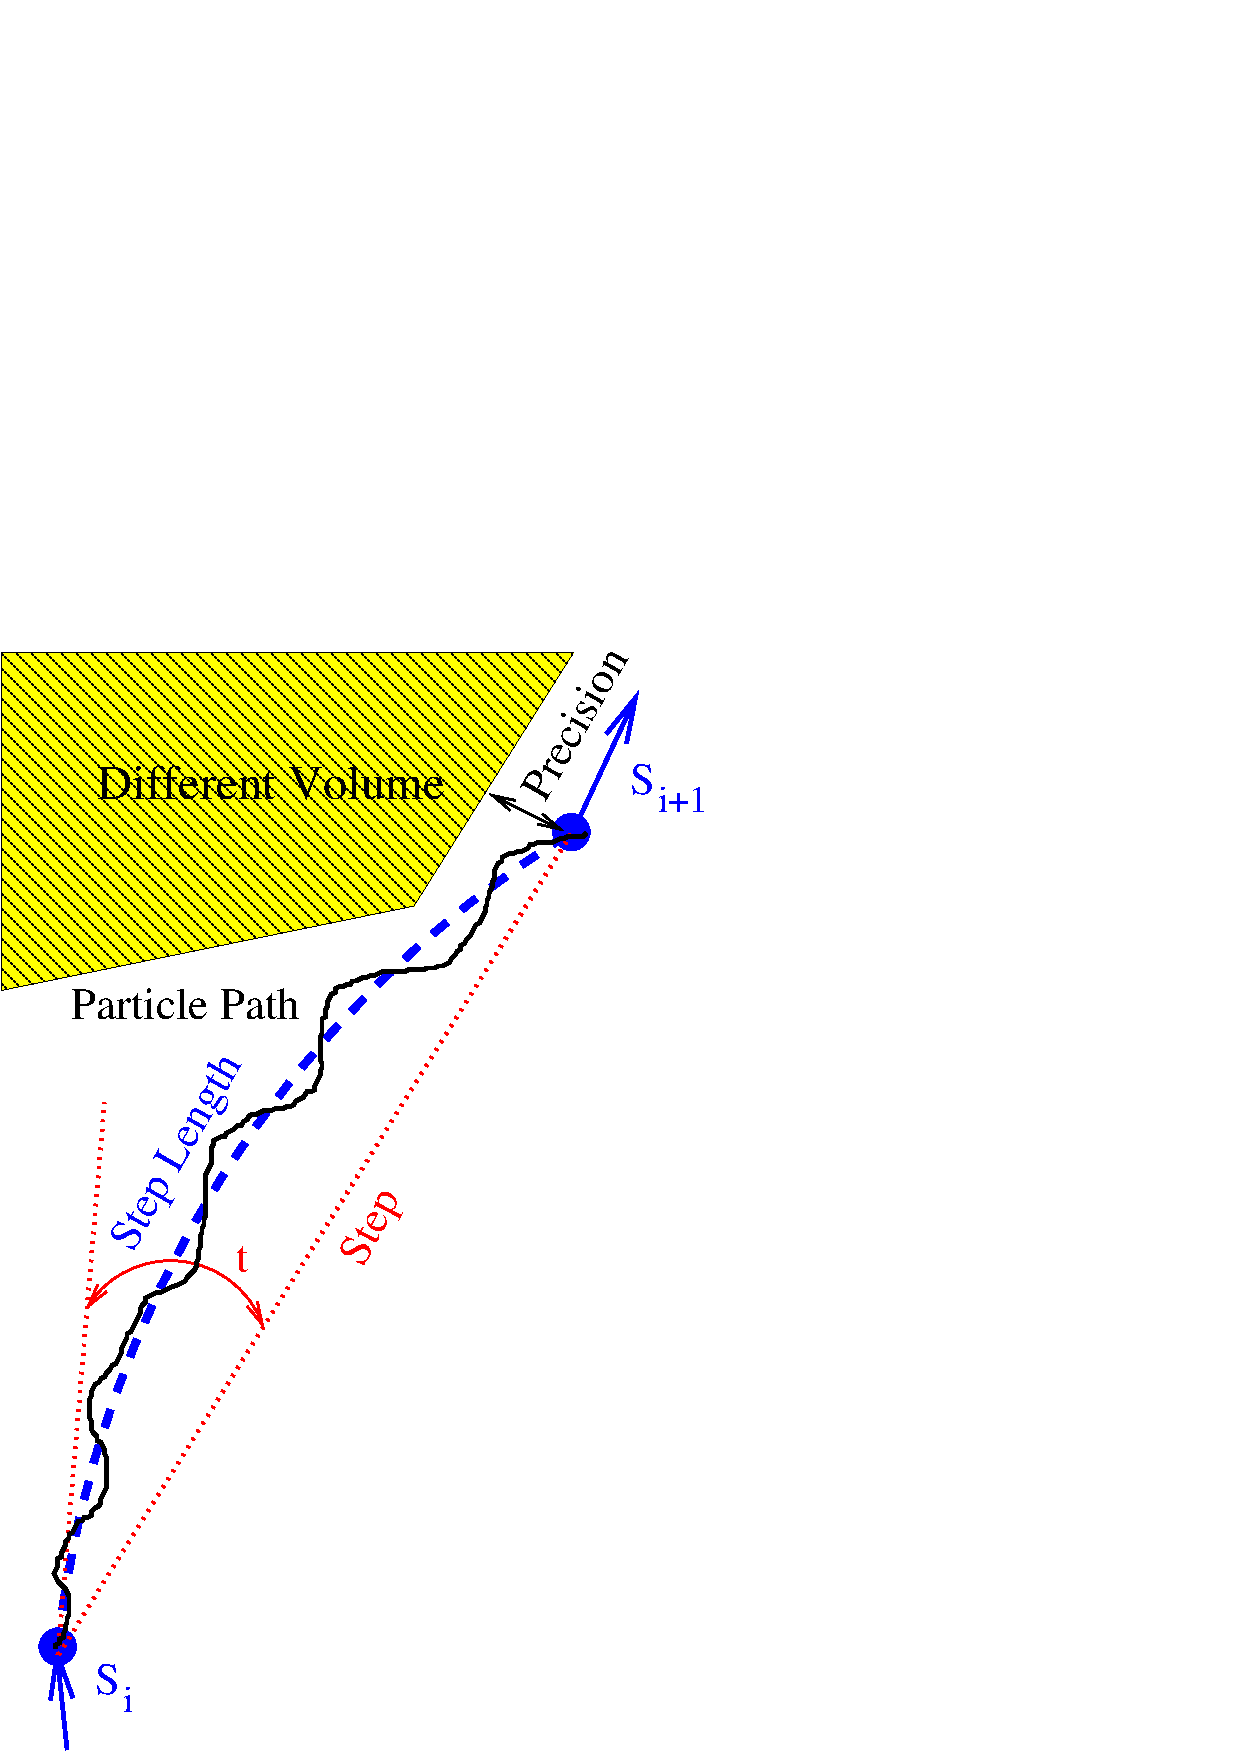
\includegraphics[width=0.5\textwidth]{figures/EMCalMCStep.pdf}
\label{fig:emcalStepManager_ParticleStep}
&
\vspace{-10.5cm}
Figure \ref{fig:emcalStepManager_ParticleStep}
An exaggerated Monte Carlo step showing some of the considerations associated
with transporting a Monte Carlo particle through a step. One step between
$s_{i}$ to $s_{i+1}$ is shown in the dotted (red) line. The dashed (blue)
line shows the step length taken due to a magnetic field. The solid (black)
line show what the particle path might really be. A new/different volume
is shown as the hashed (yellow) area. A new momentum and energy are
computed at the end of each step taking into account the energy loss
and multiple scattering. Also indicated is the deviation in the step
due to an applied magnetic field $t$, and the precision with which
the step has missed the other volume.
\\
\end{tabular*}


\paragraph{GEANT3 Switches and Settings}


GEANT3 was the first particle transport Monte Carlo integrated into
AliRoot and ROOT's virtual Monte Carlo and so has some of the
oldest and simplest interfaces. For simulation, AliRoot sets many
default settings and switches. This is done in \texttt{Config.C} which
you can find in \texttt{\$ALICE\_ROOT/macros}. There you will see a
number of line of the form \texttt{gMC->SetProcess(char *name,int value)}.
The switch names and there ALICE default values are shown in table
\ref{table:GEANT3PhysicsFlags}. There are limits both to the computer's
capabilities in dealing with the number of particles to transport and
with the physics models used by GEANT3. Consequently there are ``cuts''
used to stop the transport of particles which are below some energy
or are taking too long. The ALICE wide default values are also set
in \texttt{Config.C} using the function \texttt{gMC->SetCut(char *name,
double value)}. All of these values, and those included in the 
\texttt{galice.cuts} file are listed in table \ref{table:GEANT3PhysicsLimits}.

The \texttt{galice.cuts} file has a fixed format as indicated in
\texttt{\bf AliMC::ReadTransPar} function. In this file, lines
staring with an ``*'' are ignored. The remaining lines are required to
contain, in order separated by one or more spaces, Detector\_Name, 
Detector's\_media\_number, and then the numbered cuts and flags listed in
tables \ref{table:GEANT3PhysicsFlags} and \ref{table:GEANT3PhysicsLimits}.

\begin{longtable}{p{0.12\textwidth}p{0.1\textwidth}p{0.78\textwidth}}
  \multicolumn{3}{l}{Table \ref{table:GEANT3Switchs}} \\
      \hline \hline \\
      Switch   & \small ALICE Default values & Description \\ \hline
  \endfirsthead
      \multicolumn{3}{l}{\emph{Table \ref{table:GEANT3Switchs} continued}}\\
      \hline
      Switch   & \small ALICE Default value & Description \\
      \hline
   \endhead
      \hline
       \multicolumn{3}{r}{\emph{Table \ref{table:GEANT3Switchs} continued 
                          on next page.}}
   \endfoot
      \hline \hline
      \caption{
      %\multicolumn{3}{p{0.95\textwidth}}{Table \ref{table:GEANT3Switches}: 
               \label{table:GEANT3Switchs}GEANT3 physics process flags. 
                These flags can be set on a 
                material by material basis. The ALICE Default values are 
                set in the \texttt{Config.C} file uses the 
                \texttt{gMC->SetProcess} 
                function. The setting of these specific flags for any 
                specific material is done in 
                \texttt{\$ALICE\_ROOT/data/galice.cuts}
                file. The number on the left of the switch name is the
                column in the \texttt{galice.cuts} file that this switch
                is expected to be found. This information comes from the 
                GEANT3 documentation PHYS001-3 \cite{GEANT3:documentatoin}. 
       }
    \endlastfoot
    \footnotesize
    13 ANNI & 1 & Positron annihilation. The $e^+$ is stopped.\newline
               0 No position annihilation.\newline
               1 Positron annihilation with generation of $\gamma$.\newline
               2 Positron annihilation without generation of $\gamma$.\\
    \footnotesize
    14 BREM & 1 & bremsstrahlung. The interaction particle ($e^-$, $e^+$, 
                $\mu^-$, $\mu^+$) is stopped.\newline
               0 No bremsstrahlung. \newline
               1 bremsstrahlung with generation of $\gamma$.\newline
               2 bremsstrahlung without generation of $\gamma$.\\
    \footnotesize
    15 COMP & 1 & Compton scattering.\newline
               0 No Compton scattering.\newline
               1 Compton scattering with generation of $e^-$. \newline
               2 Compton scattering without generation of $e^-$.\\
    \footnotesize
    16 DCAY & 1 & Decay in flight. The decaying particles stops. \newline
               0 No decay in flight \newline 
               1 Decay in flight with generation of secondaries \newline
               2 Decay in flight without generation of secondaries \\
    \footnotesize
    17 DRAY & 0 & $\delta$-ray production.\newline
               0 No $\delta$-ray production.\newline
               1 $\delta$-ray production with generation of $e^-$.\newline
               2 $\delta$-ray production without generation of $e^-$.\\
    \footnotesize
    18 HADR & 1 & Hadronic interactions. The particle is stopped in case 
                of inelastic interactions, while it is not stopped in case 
                of elastic interactions.\newline
               0 No hadronic interactions.\newline
               1 Hadronic interactions with generation of secondaries.\newline
               2 Hadronic interactions without generation of 
                 secondaries.\newline
               $>2$ can be used in the user code \texttt{GUPHAD} and 
                 \texttt{GUHADR} to choose 
                 a hadronic package. These values have no effect on the 
                 hadronic packages themselves. Not supported in AliRoot.\\
    \footnotesize
    19 LOSS & 2 & Continuous energy loss.\newline
               0 No continuous energy loss, DRAY is forced to 0.\newline
               1 Continuous energy loss with generation of $\delta$-rays 
                  which have an energy above DCUTE and restricted 
                  Landau-fluctuations\cite{LandauFluct} for $\delta$-rays 
                  which have an 
                  energy below DCUTE (no $\delta$-ray produced).\newline
               2 Continuous energy loss without generation of $\delta$-rays 
                  and full Landau-Vavilov-Gauss\cite{LandauVavilov} 
                  fluctuations. In this case 
                  DRAY is forced to 0 to avoid double counting of 
                  fluctuations.\newline
               3 Same as 1, kept for backwards compatibility.\newline
               4 Energy loss without fluctuations. The value obtained 
                 from the tables is used directly.\\
    \footnotesize
    20 MULS & 1 & Multiple scattering.\newline
               0 No multiple scattering.\newline
               1 Multiple scattering according to Moliere\cite{Moiere} 
                 theory.\newline
               2 Same as 1. Kept for backwards compatibility.\newline
               3 Pure Gaussian scattering according to the Rossi 
                 formula\cite{Rossi}.\\
    \footnotesize
    21 PAIR & 1 & Pair production. The interacting $\gamma$ is 
                  stopped. \newline
               0 No pair production. \newline
               1 Pair production with generation of $e^+/e^-$.\newline
               2 Pair production without generation of $e^+/e^-$.\\
    \footnotesize
    22 PHOT & 1 & Photoelectric effect. The interacting photon is 
                  stopped.\newline
               0 No photo-electric effect. \newline
               1 Photo-electric effect with generation of $e^-$.\newline
               2 Photo-electric effect without generation of $e^-$.\\
    \footnotesize
    23 RAYL & 1 & Rayliegh effect\cite{Rayligh}. The interacting 
                  $\gamma$ is not stopped.\newline
               0 No Raylieght effect.\newline
               1 Rayliegh effect.\\
    \footnotesize
    24 STRA & 0 & Turns on the collision sampling method to simulate 
                  energy loss in thin materials, particularly gasses.\newline
               0 Collision sampling is off.\newline
               1 Collision sampling is on. \\
    \footnotesize
    PFIS & 0 & Nuclear fission induced by a photon The photon stops.\newline
               0 No photo-fission.\newline
               1 Photo-fission with generation of secondaries.\newline
               2 Photo-fission without generation of secondaries.\\
    \footnotesize
    MUNU & 1 & Muon-nucleus interactions. The muon is not stopped.\newline
               0 No muon-nucleus interactions.\newline
               1 Muon-nucleus interactions with generation of 
                 secondaries.\newline
               2 Muon-nucleus interactions without generation of secondaries.\\
    \footnotesize
    CKOV & 1 & Light absorption. This process is the absorption of light 
                photons in dielectric materials. It is turned on by default 
                when the generation of $\check{C}$erenkov\cite{Cerenkov} 
                light is requested (in GEANT manual it is LABS).\newline
                0 No absorption of photons.\newline
                1 Absorption of photons with possible detection.\\
    \footnotesize
    SYNC & 0 & Synchrotron radiation in magnetic fields.\newline
               0 Synchrotron radiation is not simulated.\newline
               1 Synchrotron photon are generated, at the end of the 
                 tracking step.\newline
               2 Photons are not generated, the energy is deposited 
                 locally.\newline
               3 Synchrotron photons are generated, distributed along the 
                 curved path of their particle. \\
   \normalsize
   \label{table:GEANT3PhysicsFlags}
\end{longtable}

\begin{longtable}{p{0.15\textwidth}p{0.2\textwidth}p{0.65\textwidth}}
  \multicolumn{3}{l}{Table \ref{table:GEANT3PhysicsLimits}} \\
      \hline \hline \\
      Parameter   & \small ALICE Default value & Description \\ \hline
  \endfirsthead
      \multicolumn{3}{l}{\emph{Table \ref{table:GEANT3PhysicsLimits} 
                         continued}}\\
      \hline
      Parameter   & ALICE Default value & Description \\
      \hline
   \endhead
      \hline
       \multicolumn{3}{r}{\emph{Table \ref{table:GEANT3PhysicsLimits} 
                          continued on next page.}}
   \endfoot
      \hline \hline
      \caption{\label{table:GEANT3PhysicsLimits}GEANT3 physics process limits. 
                These ``cuts'' can be set on a 
                material by material basis. The ALICE Default values are 
                set in the \texttt{Config.C} file uses the 
                \texttt{gMC->SetCuts} 
                function. The setting of these specific flags for any 
                specific material is done in 
                \texttt{\$ALICE\_ROOT/data/galice.cuts}
                file. The number on the left of the cut name is the
                column in the \texttt{galice.cuts} file that this cut
                is expected to be found. This information comes from the 
                GEANT3 documentation ZZZZ010-2 \cite{GEANT3:documentatoin}
      }
    \endlastfoot

    \footnotesize
    3 CUTGAM & $1.\times 10^{-3}$ GeV & Threshold for gamma transport.\\
    \footnotesize
    4 CUTELE & $1.\times 10^{-3}$ GeV & Threshold for electron and positron 
                                   transport.\\
    \footnotesize
    5 CUTNEU & $1.\times 10^{-3}$ GeV & Threshold for neutral hadron 
                                         transport.\\
    \footnotesize
    6 CUTHAD & $1.\times 10^{-3}$ GeV & Threshold for charged hadron 
                                        and ion transport.\\
    \footnotesize
    7 CUTMUO & $1.\times 10^{-3}$ GeV & Threshold for muon transport.\\
    \footnotesize
    8 BCUTE &  $1.\times 10^{-3}$ GeV & Threshold for photons produced by 
                                   electron bremsstrahlung.\\ 
    \footnotesize
    9 BCUTM &  $1.\times 10^{-3}$ GeV & Threshold for photons produced by 
                                   muon bremsstrahlung.\\ 
    \footnotesize
    10 DCUTE &  $1.\times 10^{-3}$ GeV & Threshold for electrons produced by 
                                    electron $\delta$-rays.\\ 
    \footnotesize
    11 DCUTM &  $1.\times 10^{-3}$ GeV & Threshold for electrons produced by 
                                    muon or hadron $\delta$-rays.\\ 
    \footnotesize
    12 PPCUTM & $1.\times 10^{-3}$ GeV & Threshold for $e^{\pm}$ direct pair 
                                    production by muons.\\
    \footnotesize
    TOFMAX & $1.\times 10^{10}$ sec & Threshold on time of flight counted 
                                       from primary interactions time.\\ 

   \label{table:GEANT3PhysicsLimits}
\end{longtable}

\paragraph{GEANT4 Switches and Settings}

\paragraph{Fluka Switches and Settings}

%
\begin{thebibliography}{99}
\bibitem{GEANT3:documentatoin} CERN Program Library. 
         \textsl{GEANT Detector description and Simulation Tool},
         CERN Program Library Long writeup W5013, October 1994
\bibitem{GEANT4} GEANT4 Working Group, ``User Documentation'',
                 Accessed Feb. 4 2013. 
                 http://geant4.cern.ch/support/suerdocumentatoin.shtml
\bibitem{Fluka}  FLUKA Team, ``FLUKA'', Access Feb. 4 2013,
                 http://www.fluka.org/fluka.php?id=man\_onl
\bibitem{LandauFluct} \textsl{GEANT Detector description and Simulation Tool},
                      PHYS332. and
                      L. Landau. \textsl{On the Energy Loss of Fast Particles 
                      by Ionisation}, J. Phys. 8:201, 1944. and
                      K. S. K$\ddot{o}$lbig and B. Schorr. \textsl{Asymptotic 
                      expansion for the Landau density and distribution 
                      functions}, Comp. Phys. Comm., 32:121,1984
\bibitem{LadauVavilov}\textsl{GEANT Detector description and Simulation Tool},
                       PHYS332. and 
                       P. V. Valilov. \textsl{Ionisation losses of high 
                       energy heavy particles}, Soviet Physics 
                       JETP, 5:749, 1957
\bibitem{Moliere}\textsl{GEANT Detector description and Simulation Tool},
                 PHYS320. and
                 G. Z. Moliere \textsl{Theorie de Streuung schneller 
                 geladener Teilchen I: Enzelstreuung am abgerschmitten 
                 Coulomb-Feld},Z. Naturforsch., 2a:133, 1947 and
                 G. Z. Moliere, \textsl{Teeorie der Steuung schneller 
                 geladerner Teichen II: Merfach- und Vielfachstreuung} 
                 Z. Naturforsh., 3a:87, 1948 and
                 W. T. Scott. Rev. Mod. Phys. 35:231 1963
\bibitem{Rossi}\textsl{GEANT Detector description and Simulation Tool},
                 PHYS320 and
                 R. Rossi, Prentice-Hall, Englewoood Clifgs, 1962
                 R. Rossi, and K. Greisen, Rev. Mod. Physics, 13-240, 1942
\bibitem{Rayliegh} \textsl{GEANT Detector description and Simulation Tool},
                   PHYS250. and
                   W. R. Nelson, H. Hiayama, and D. W. O. Rogers. Technical 
                   Report 265, SLAC, 1985
\bibitem{Cerenkov} \textsl{GEANT Detector description and Simulation Tool},
                   PHYS260,
                   J. D. Jackson \textsl{Classical Electrodyanamics}, 
                   J. Wiley et Sons, Inc. New York, 1975
\end{thebibliography}
%
%\end{document}
%

\clearpage


\subsection{Digitization: SDigits and Digits - Evi \label{sec:digi}}

We want to generate events which look like the real data collected
by the experiment. In the end, we want to have an amplitude in ADC
counts and a time (when particle traverse a cell) per each cell (tower)
of the calorimeter. In the code for calorimeters, it is done in the
following steps: 
\begin{enumerate}
\item \textbf{SDigit} objects are created, they consist
of the sum of deposited energy by all Hits in a cell (a particle can
create Hits in different cells but only one in a single cell), so
there is only one SDigit per fired cell.
\item \textbf{Digit} objects are created, they are like the SDigits but the energy in the cell
is transformed into the ADC amplitude units, the electronic noise
is added and Digits whose energy does not pass an energy threshold
(3 ADC counts) are eliminated. SDigits and Digits are stored in the files
\textbf{EMCAL.SDigits.root} and \textbf{EMCAL.Digits.root}, respectively.
\end{enumerate}

\subsection{Raw data - David \label{sec:simu_raw}}

The experiment does not record Digits directly, but instead a series of so-called
time samples with 10-bit ADC counts per channel. Each time bin is 100 ns
wide, corresponding to a 10 MHz readout.
These samples are referred to as
\textbf{Raw Data}. The samples follow a certain signal shape, more complicated than
a Gaussian distribution, which is fitted offline. 
The simulated signal (Gamma-2) shape is described in the AliEMCALRawResponse class,
in the RawResponseFunction method.
With real data, which is zero-suppressed, i.e. has the pedestal subtracted online, the
Digits amplitude is just the maximum of the distribution obtained
with the fit to the sample. The Digit time (defined by the time the
particle hits the active volume of the detector) is the time value at
the maximum signal fit. There are methods to go from Digits to
Raw and vice versa in the AliEMCALRawUtils class: Raw2Digits and Digits2Raw,
respectively. For the reconstruction step Digits are needed. The
generation of Raw Data is optional during simulations and the generated 
data can be reconstructed directly from Digits, but Raw data is the initial
step when reconstructing real data.


\subsection{How to make a simulation\label{sec:simu_steps}}

TestEMCALSimulation.C is a very simple macro where we specify all the simulation parameters
and proccess the simulation. Below is a similar but a bit more elaborated macro:



\begin{DDbox}{\linewidth}
\begin{lstlisting}
void TestEMCALSimulation() {

TString detector=``EMCAL TPC''; // Define in this variable the detectors that you want to be included in the simulation for the digitization. They can be less detectors than the detectors defined in the Config.C file, imagine that you want all the detectors in front of EMCal present to consider the conversion of particles but you are not really interested in the output from these detectors. 
// Option detector=``ALL''  makes all detectors. 

AliSimulation sim ; //Create simulation object 

// Generation and simulation 

sim.SetRunGeneration(kTRUE) ; //Default value is kTRUE, make generation  
// For some reason we may want to redo the Digitization, without redoing the generation, in this case it must set to kFALSE 

// Making SDigits 
sim.SetMakeSDigits(detector) ; //We want to make SDigits
// set no detectors if SDigits are already made

// Making Digits 
sim.SetMakeDigits(detector) ; //We want to make Digits 
// set no detectors if SDigits are already made

//Merging 
//sim.MergeWith(``bgrd/galice.root'') ; //If we want to merge a signal and a background, the merging is done at the SDigit level. The background must be located in the repertory defined in the method. 

//Write Raw Data, make Raw data from digits 
//sim.SetWriteRawData(detector) ;
//sim.SetConfigFile(``somewhere/ConfigXXX.C'');//Default is Config.C

//Make the simulation 
sim.Run(3) ; // Run the simulation and make 3 events 



\end{lstlisting}
\end{DDbox}
\clearpage



\section{Reconstruction code}


The energy deposited by the particles in the towers produces scintillating light that is propagated with optic fibers through the different layers to APD placed at the base of the cells. The APDs amplify the signal and generate an electronic pulse shape that is stored in the raw data format. From this pulse shape, we extract the signal amplitude and the arrival time. The pulse shape is fitted during the reconstruction via a parametrized function and TMinuit, and those 2 values are extracted.

A particle produces signals in different towers (electromagnetic shower expands more than its Moli\`ere radius which is a cell size). The next step is the formation of clusters of cells that belong to the same particle, although depending on the energy, granularity, clusterization algorithm or event type, those clusters might have contributions from different particles. The default algorithm in pp collisions is a simple aggregation of neighboring cells until there is no more cells above a certain energy threshold (named {\it clusterizer V1}). In case of Pb-Pb collisions environment, where particle showers merge quite often, we apply another algorithm that aggregates cells to the clusters until reaching a cell with more energy than the precedent (named {\it clusterizer V2}). Depending on the analysis type, one might want to use one or the other clusterization type. For this reason, a re-clusterization is also possible at the analysis level. A last clusterizer is implemented, which makes 3x3 clusters. It has been used in jet analysis for instance in order to avoid biasing jet reconstruction where one is interested in the energy flow over a large area without explicit reconstruction of photon showers and where the driving consideration is that the wide clusterizer does not interfere with the jet finder. For $\pi^{0}$, $\eta$, and direct $\gamma$ analyses, {\it V2} is most likely preferable).

Once the cluster is defined, we calculate cluster parameters, shower shape parameters, that will help at the analysis level to identify each cluster as one particle type. Also, we compare the cluster position information with the propagation of tracks measured in the central barrel to the EMCAL surface, to identify the clusters generated by charged particles.

The final analysis objects, ESDs and AODs, contain all the cluster and cell basic informations allowing to redo the clusterization if needed at the analysis level.

%The class AliReconstruction manages this part. This step can
%begin either from the Digits or from the Raw data. We can distinguish
%different steps described in the following sections. 


\subsection{Offline data base access}

How to create explained OCDB/OADB section.

\subsubsection{Energy calibration}

\subsubsection{Bad channels - Marie, Alexis}

\subsubsection{Alignment - Marco}

\subsection{Raw data fitting: from ADC sample to digits - David}

As also discussed in Sec.~\ref{sec:simu_raw}, the recorded Raw data consists
of instead a series of so-called time samples with 10-bit ADC counts per channel. 
Each time bin is 100 ns wide, corresponding to a 10 MHz readout.
The expected signal (Gamma-2) shape is described e.g. in the AliEMCALRawResponse class,
in the RawResponseFunction method.
The reconstruction from Raw data to Digits is done in the AliEMCALRawUtils class,
Raw2Digits method.
The Raw ADC time samples data is kept in AliCaloBunchInfo objects, which are given
as input to an AliCaloRawAnalyzer object, which returns the signal amplitude and time
information (in the form of an AliCaloFitResults object).
There are several different AloCaloRawAnalyzer versions, which can be selected via
AliEMCALRawUtils::SetFittingAlgorithm(). They are:

\begin{itemize}
 \item kStandard:
   AliCaloRawAnalyzerKStandard, which is a (slower but simple) Gamma-2 fit implementation.
 \item  kFastFit: 
   AliCaloRawAnalyzerFastFit, which is a faster Gamma-2 fit implementation from Aleksei Pavlinov.
 \item kNeuralNet:
   AliCaloRawAnalyzerNN, which is a neural network implementation from Paola La Rocca and Franco Riggi.
 \item kPeakFinder:
   AliCaloRawAnalyzerPeakFinder, which is a fast (parameterized vector operations) implementation from Per Thomas Hille. 
 \item kCrude:
   AliCaloRawAnalyzerCrude, which is the simplest possible algorithm: just take the maximum ADC value as the signal amplitude.
 \item kFakeAltro:
   AliCaloRawAnalyzerFakeALTRO, which is an algorithm intended for the Trigger/TRU raw data analysis, i.e. not for the regular FEE or cell/tower data.
\end{itemize}



\subsection{Clusterization: From digits to clusters - Adam}


%\subsection{Clusterization: From digits to clusters -  Adam}
%classes:
%AliEMCALClusterizer.cxx
%AliEMCALClusterizerv1.cxx
%AliEMCALClusterizerNxN.cxx
%AliEMCALClusterizerv2.cxx
%AliEMCALClusterizerFixedWindow.cxx  
%unfolding
The set of information related to one cell - (between each other) the position of cell and the energy deposited in it is called a digit. The digit is represented by the \texttt{AliEMCALDigit} class. A group of digits which are related somehow between each other is called a cluster. The cluster is represented by the \texttt{AliEMCALRecPoint} class.

Transformation from digits to clusters is done during clusterization phase. There are many ideas how to form cluster. Each applied idea is called clusterizer. Currently, there are four types of clusterizers in the EMCal:

%\parskip

\begin{itemize}
%\parskip
\item Clusterizer V1,
\item Clusterizer V2.
\item Clusterizer V1 with unfolding,
\item Clusterizer NxN,

\end{itemize}


Technically it is organized in the following way. \texttt{AliEMCALClusterizer} is a base clusterizer class. The V1 and NxN clusterizer classes (\texttt{AliEMCALClusterizerv1} and \texttt{AliEMCALClusterizerNxN}, respectively) inherit from the base class. The clusterizer class V2 (\texttt{AliEMCALClusterizerv2}) inherits from \texttt{AliEMCALClusterizerv1}. The third case of clusterization (clusterizer V1 with unfolding) is realized via settable option in the \texttt{AliEMCALClusterizerv1} class. The dedicated class \texttt{AliEMCALUnfolding} was written for the purpose of unfolding. The description of each clusterizer type separately and common clusterization structure together with a description of the cluster is explained below.
\subsubsection{Clusterization in the EMCal}
A clusterizer is called in the \texttt{AliEMCALReconstructor} class. The set of clusterizer parameters is initialised. Usually parameters are taken from the OCDB. The full set of parameters which are used during clusterization is given in Tab.~\ref{tab:clusterizationparams}. The other fields of the \texttt{AliEMCALClusterizer} class are given in Tab.~\ref{tab:clusterizationfields}.
%
\begin{table}[!h]
\begin{center}
  \begin{tabular}{| c | c | l |}
  \hline
  Name & Type & Explanation \\ 
  \hline
   fTimeMin                & \texttt{Float\_t } & minimum time of physical signal in a cell/digit\\
   fTimeMax                & \texttt{Float\_t } & maximum time of physical signal in a cell/digit\\
   fTimeCut                & \texttt{Float\_t } & maximum time difference between the digits inside EMC cluster\\
   fToUnfold               & \texttt{Bool\_t  } & says if unfolding should be performed \\
   fECAClusteringThreshold & \texttt{Float\_t } & minimum energy to seed a EC digit in a cluster\\
   fECALocMaxCut           & \texttt{Float\_t } & minimum energy difference to distinguish local maxima in a cluster\\
   fECAW0                  & \texttt{Float\_t } & logarithmic weight for the cluster center of gravity calculation\\
   fMinECut                & \texttt{Float\_t } & minimum energy for a digit to be a member of a cluster\\
   fSSPars[8]              & \texttt{Double\_t} & shower shape parameters \\
   fPar5[3]                & \texttt{Double\_t} & shower shape parameter 5\\
   fPar6[3]                & \texttt{Double\_t} & shower shape parameter 6\\
  \hline
  \end{tabular}
\end{center}
\caption{Parameter name, type and explanation.}
\label{tab:clusterizationparams}
\end{table}
%
\begin{table}[!h]
\begin{center}
  \begin{tabular}{| c | c | l |}
  \hline
  Name & Type & Explanation \\ 
  \hline
    fADCchannelECA     &  \texttt{Float\_t}         &  width of one ADC channel for EC section (GeV)\\
    fADCpedestalECA    &  \texttt{Float\_t}         &  pedestal of ADC for EC section (GeV)\\
    fTimeECA           &  \texttt{Float\_t}         &  calibration parameter for channels time\\
    fIsInputCalibrated &  \texttt{Bool\_t}          &  to enable reclusterization from ESD cells\\
    fJustClusters      &  \texttt{Bool\_t}          &  false for standard reco                  \\
    fDigitsArr    & \texttt{TClonesArray*}          &  pointer to array with EMCAL digits       \\
    fTreeR        & \texttt{TTree*}                 &  pointer to tree with output clusters                                         \\
    fRecPoints    & \texttt{TObjArray*}             &  pointer to array with EMCAL clusters                                         \\
    fGeom         & \texttt{AliEMCALGeometry*}      &  pointer to geometry for utilities                                            \\
    fCalibData    & \texttt{AliEMCALCalibData*}     &  pointer to calibration database if available                                  \\
    fCaloPed      & \texttt{AliCaloCalibPedestal*}  &  pointer to tower status map if available                                      \\
    fDefaultInit         & \texttt{Bool\_t}          &  says if the task was created by default ctor \\
    fNumberOfECAClusters & \texttt{Int\_t}           &  number of clusters found in EC section \\
    fClusterUnfolding & \texttt{AliEMCALUnfolding*} &  pointer to unfolding object \\
\hline
  \end{tabular}
\end{center}
\caption{Other fields in the \texttt{AliEMCALClusterizer} class.}
\label{tab:clusterizationfields}
\end{table}
%
Also input and output are connected. Finally, a clusterization phase is done in a \texttt{Digits2Clusters} method. Main steps run as follow:
\begin{enumerate}
\item Get calibration parameters (method \texttt{GetCalibrationParameters}),
\item Get pedestal parameters (method \texttt{GetCaloCalibPedestal}),
\item Make clusters (method \texttt{MakeClusters}),
\item Make unfolding or not (method \texttt{MakeUnfolding}),
\item Evaluate cluster properties (\texttt{AliEMCALRecPoint} class methods),
\item Store clusters.
\end{enumerate}
In the first two steps calibration (ADC counts to energy conversion) and pedestal parameters are read from a database. The third step, where clusters are formed, is different for each clusterizer. 
However, some beginning parts of this step are common for each algorithm. The input is the same. It is an array of fired digits with electronic signal registered in each of them. Also calibration and cleaning the array of digits, to work with reduced sample of digits, is the same for each algorithm. This common part is done in the common method \texttt{Calibrate} of the \texttt{AliEMCALClusterizer} class. Here, we require the proper timing (via selection of \texttt{fTimeMax} and \texttt{fTimeMin} of a given digit), status (check of dead channel map) and calibrate energy and time of each digit. If any digit fails to pass one of requirement it is rejected from a ``working array'' of digits (pool of digits). In make clusters step the \texttt{AreNeighbours} method is used. The method could differ for each clusterization algorithm. 
%Also the used method \texttt{AreNeighbours} differs for each clusterizer in this step. 
The explanation how clusters are formed is given in next four subsections for each clusterization algorithm, respectively. The next step (unfolding) is an option in each clusterizer, but currently is used only for the V1 clusterizer. The last two steps (evaluation of a cluster properties and its recording) are the same for each algorithm.

\subsubsection{Clusterizer V1}
%The input for each clusterizer is array of fired digits with electronic signal registered in each of them. The first step in each algorithm is to calibrate and clean array of digits to work with reduced sample of digits. It is done in common method \texttt{Calibrate} of \texttt{AliEMCALClusterizer} class. Here we require the proper timing (via selection of \texttt{fTimeMax} and \texttt{fTimeMin} of a given digit), status (check of dead channel map) and calibrate energy and time of each digit. If any digit fails to pass one of requirement it is rejected from a ``working array'' of digits. 
%Then, in the V1 algorithm, we reject digits with energy smaller than \texttt{fMinECut}, which is set to be by default 10~MeV in the database. 
Having obtained ``working array'' of digits in the V1 algorithm we additionally reject digits with energy smaller than \texttt{fMinECut}, which is set to be 10~MeV in the database by default.

After selecting digits we form clusters. We loop over all digits to find the first seed digit with energy grater than \texttt{fECAClusteringThreshold} (default value is 100~MeV). 
When the seed digit is found it is associated to a new cluster and removed from the ``working array'' of digits. We loop over all remaining digits to look for neighbours of the seed digit.
The neighbour digits are called digits which have at least common side (i.e.: row index difference or column index difference must be equal 1, but not both of them at the same time are equal 1, so one cell can have four neighbours at maximum).
The additional requirement on neighbour digits is applied. The absolute value of time difference for two digits must be less or equal \texttt{fTimeCut}.

The neighbour digits are associated to the cluster (also removed from the ``working array'' of digits) and we keep on looking for neighbours of each digit associated to the cluster. When a digit is associated to one cluster it cannot be associated to other one. When there are no more neighbours of digits in one cluster one can say that this cluster is formed. Once the cluster
is formed and there are still remaining digits in the ``working array'' the procedure starts to check seeds and all the story repeats until no seed digit is found. The consequence of such algorithm is that one cluster can contain all digits in the super-module. The other thing is that there can be digits which are not associated to any cluster. The special case when cluster is formed from digits in two super-modules at the same SM-$\phi$ angle is also supported.  



\subsubsection{Clusterizer V2}
%The first step in this algorithm is the same as in V1 clusterizer. It is calibration of digits to get the pool of digits with the energy over the energy threshold \texttt{fMinECut} and with proper timing (\texttt{fTimeMax} and \texttt{fTimeMin} variables). 
%When it is done the most energetic digit with the energy over \texttt{fECAClusteringThreshold} is taken. It is the seed of a cluster. 
The algorithm starts with the pool of digits. Then the most energetic digit with the energy over \texttt{fECAClusteringThreshold} is taken. It is the seed of a cluster. 
We scan over digits already associated to the cluster and check for neighbours. It is the iterative procedure. Here, the absolute value of the time difference of seed and neighbours digits should be less or equal \texttt{fTimeCut}. The definition of neighbours is the same like in V1 clusterizer, however, energy of neighboring digit should be smaller in order to become a neighbor. \texttt{fDoEnGradCut} flag is responsible for application of the last condition. 
If the process of one cluster formation ends we start from the point where new and the most energetic digit is found in the pool of digits and repeat other steps until no digit remains in the pool.

\subsubsection{Clusterizer V1 with unfolding}
The main goal of unfolding is to divide multi-maxima clusters into single-maxima clusters and split energy of unfolded clusters. The unfolding is an option which is switched off by default. It can be switched on in every clusterizer. However, as the output of V2 and NxN algorithms clusters are already small and contains only one maximum. The V1 clusterizer provides multi-maxima clusters, so unfolding can be reasonably used only in V1 method of clusterization. 

Unfolding uses already reconstructed clusters from V1 as an input and modify (split and share energy in digits among several clusters) them if necessary. The unfolding scheme can be divided into several steps:
%\parskip
\begin{enumerate}
%\parskip
\item Maxima finding.
\item Fit.
\item Reclustering.
\end{enumerate}
{\bf Maxima finding.} As the first step number of local maxima is defined in one cluster. A cell is a local maximum when its energy deposit is greater than the energy deposit in each of its neighboring cells (by neighboring cell we understand here two cells touched by side or corner, so one cell can have 8 neighbours at maximum) by at least some constant value. This constant value  is called the minimum energy difference between two local maxima (\texttt{fECALocMaxCut}) and as a default is equal to 30~MeV. In the particular case where two neighboring cells have a similar energy deposit (the difference between energy of two cells is below a certain value) the cluster is treated as a flat one with no maximum.

The outcome of the maximum finding procedure is divided in two cases. In the case no pronounced maximum or only one maximum is found unfolding is not applied and cluster is not touched. If there are at least two maxima the procedure of unfolding starts running.

{\bf Fit.} The next step is the fitting procedure which allows to disentangle overlapping clusters based on the knowledge of what should be the typical shower shape of a $\gamma$ particle. The energy distribution in a single photon cluster (shower shape) is described by following function:
\begin{equation}
\label{eq:function}
f(r)=P_0 \cdot exp(- (2.332 \cdot r)^{P_1} \cdot (\frac{1}{P_3 +P_4 \cdot (2.332 \cdot r)^{P_1} } + \frac{P_5}{1+(2.332 \cdot r)^{P_2} \cdot P_6} ) ), 
\end{equation}
where $P_{0,1,2,3,4,5,6}$ are parameters and $r$ is a distance between a cell center and the center of gravity of a cluster. This function is constant for given $\phi$ region and it is our reference to start to unfold clusters. One single photon cascade can be described by the shower shape function with fixed parameters. However to locate it in the detector we need 3 parameters: position of center of gravity of cluster in $\phi$ and $\eta$ coordinates and a cluster's energy. In case of a single photon cluster we could fit just mentioned 3 parameters. If there are more maxima we start with more parameters. The correlation is very simple. One maximum found corresponds to 3 parameters which we want to fit. The initial value of parameters for one maximum are following: position of the local maximum cell in $\phi$ and $\eta$ coordinates and its energy. TMinuit package is called to minimize the $\chi^2$ between the shower shape function of a single $\gamma$ and the shower shape spectrum of the cluster being unfolded. The outcome of the fit is the set of parameters which describe center of gravity and energy of each unfolded cluster.

{\bf Reclustering.} The last step is to build in terms of cell energy attribution the two (or more) clusters obtained splitting the original big blob cluster. There is an obvious constraint for the energy in each cell. The sum of the energies associated to the different clusters returns the measured energy associate at the cell. For each cell, and for each split cluster, the fit result from the previous step provides an expected value which can be used as weight to distribute the cell energy among the different unfolded clusters. The total (measured) signal present in the cell is shared among the split clusters with the proportion given by the fit function values. The split (unfolded) clusters are built based on these new cell entries. 

The energy of each cell in the unfolded cluster should be above a certain energy threshold $E_{th}$ (\texttt{fThreshold}). By default energy threshold is set to be $E_{th}=10$~MeV. If a cell after unfolding in a given cluster has an energy below threshold, this cell is rejected from this cluster and its energy is shared among other clusters, proportionally to the energy of this cell in other clusters. If after unfolding only one cluster contains a cell with energy above threshold cells below threshold are rejected from other clusters and the full energy is associated to the cell with energy above threshold. If after unfolding each energy of cell is below threshold then the whole energy is associated to the most energetic cell.

The number of new (unfolded) clusters will be the same as the number of local maxima found during the first step above. When unfolding succeeds the original big blob cluster is replaced by several unfolded clusters. Unfolding method is precisely described in~\cite{unfolding_note}.
%
%Different methods of clusterization are compared in Fig.~\ref{fig:clusterizers}.
\begin{figure}[!h]
\begin{center}
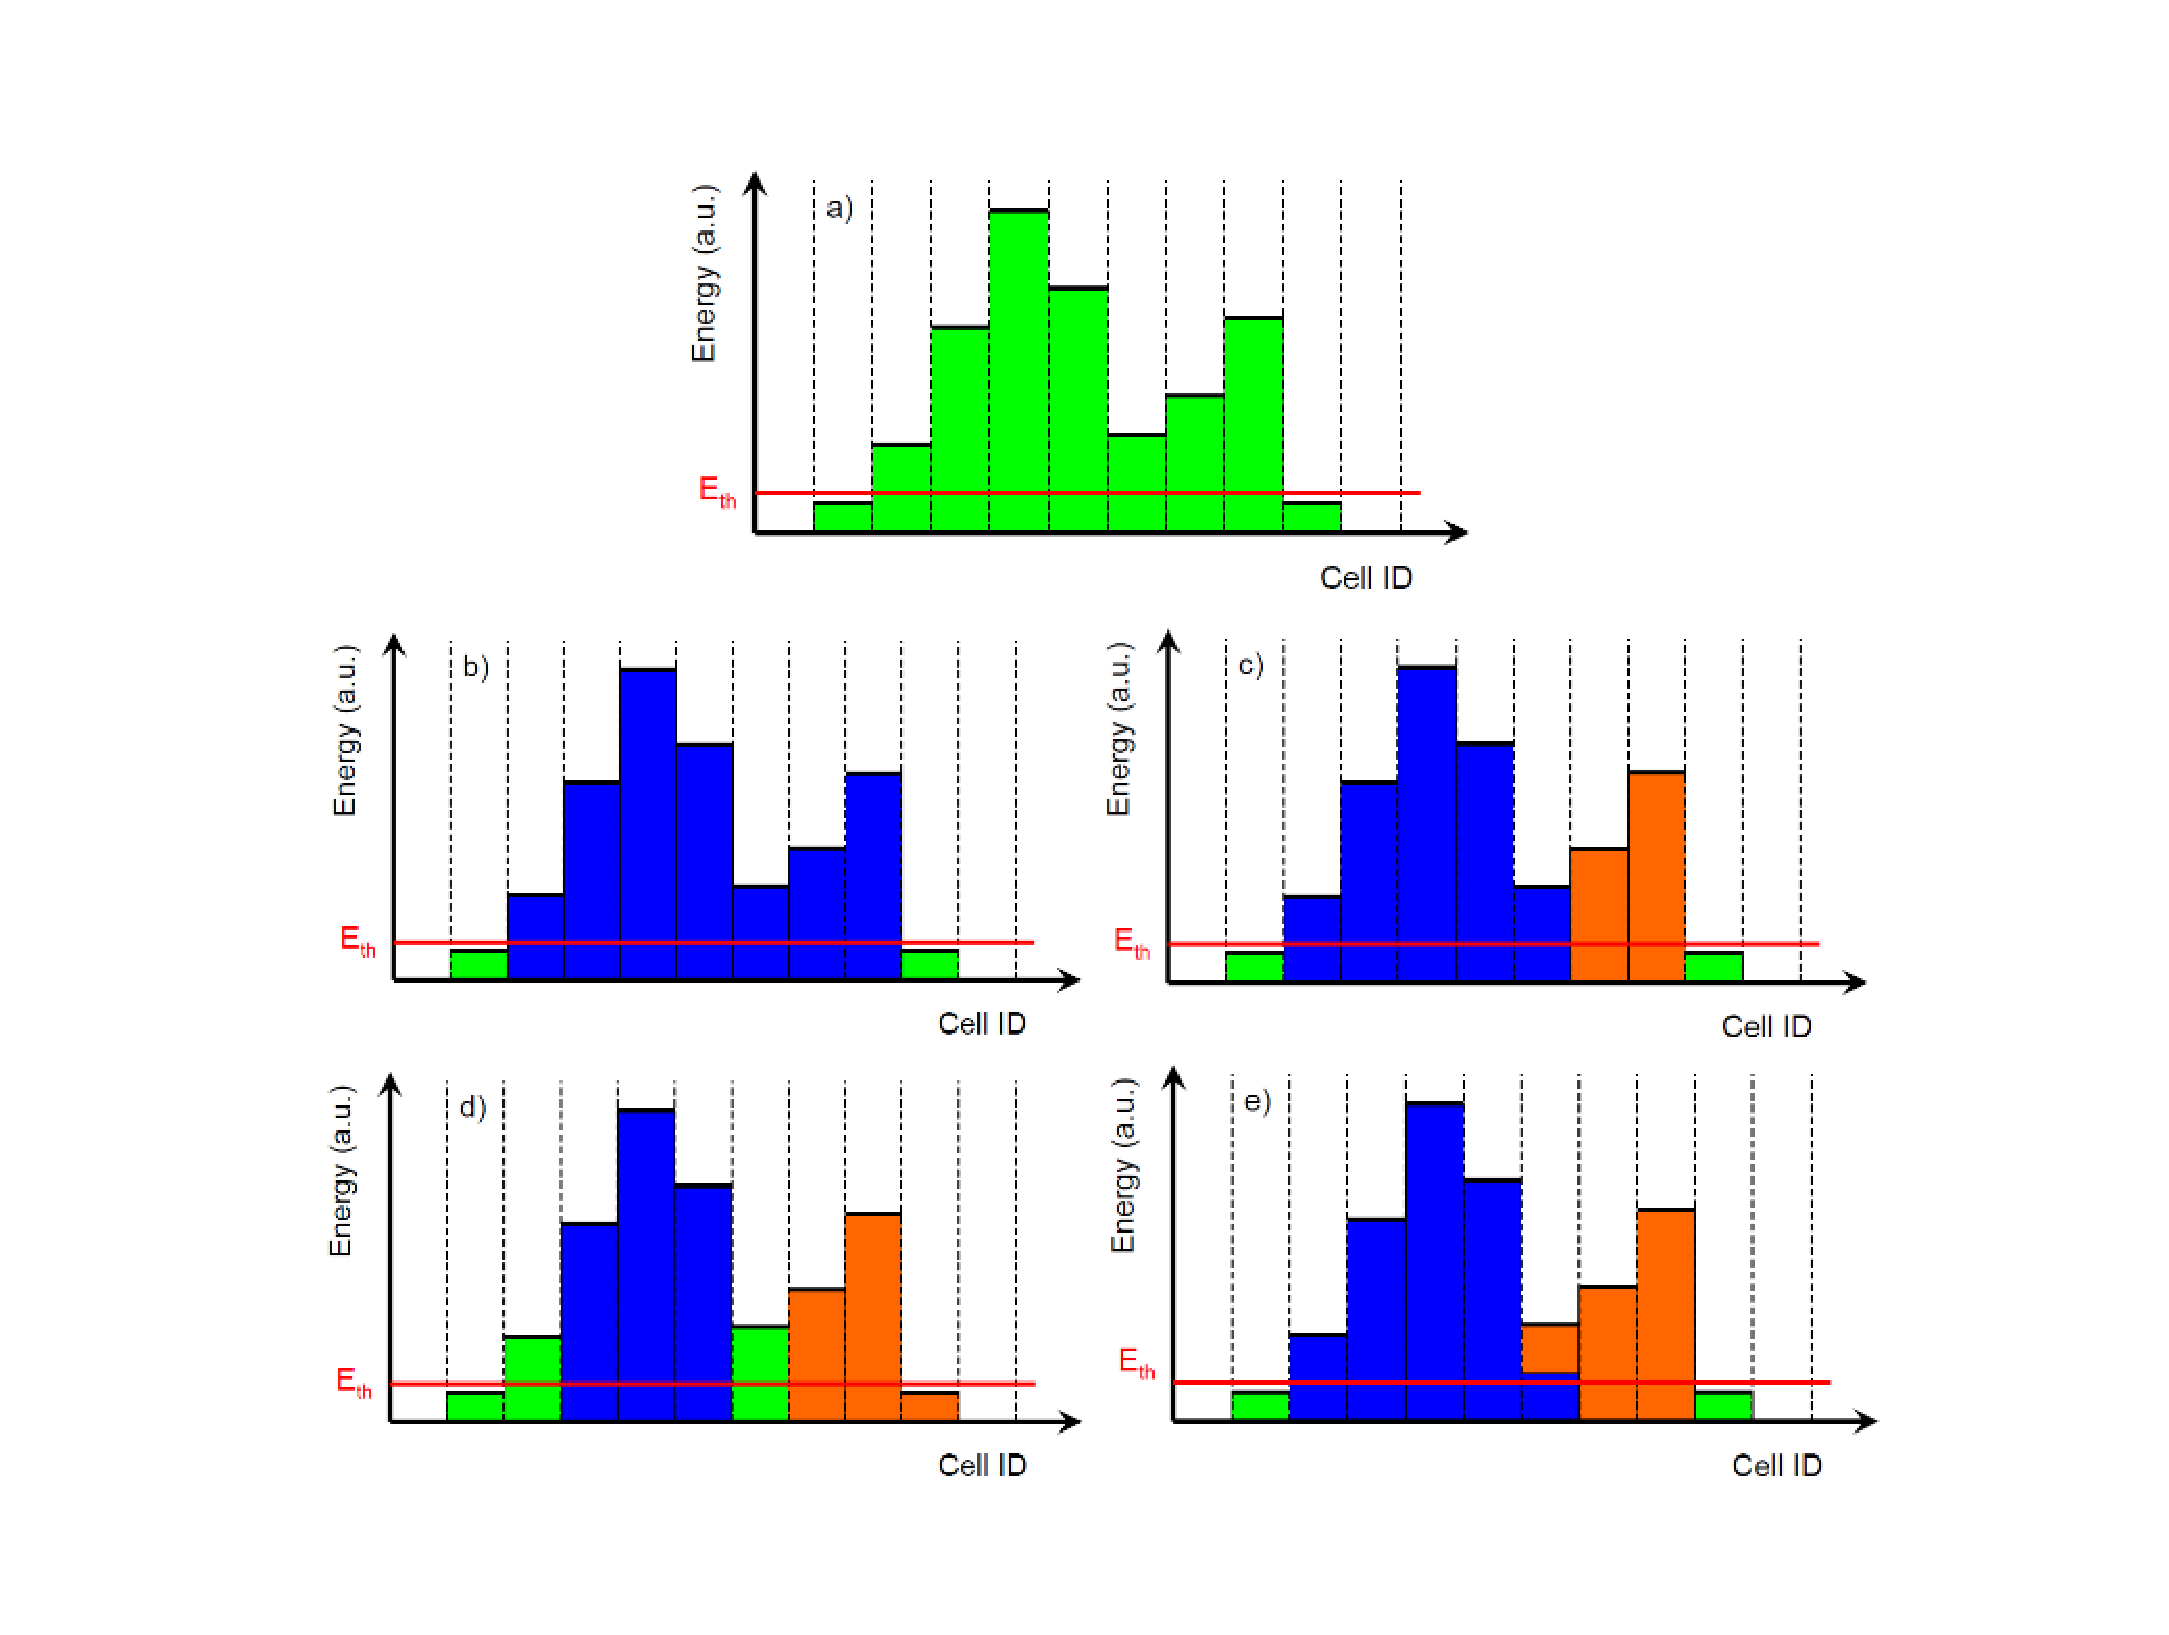
\includegraphics[scale=0.4]{figures/clusters}
\caption{Comparison of different algorithms of clusterization. Boxes represent energy in cells. $E_{th}$ is clusterization threshold \texttt{fMinECut}. a) Energy in cells before clusterization marked by green color. b) Result of V1 clusterizer. There is one big cluster made of cells in blue color. Green cells are below threshold and not associated to the cluster. c) Result of V2 algorithm. There are two clusters made of blue and orange cells. Green cells are below threshold and not associated to any cluster. d) Result of NxN clusterizer. There are two clusters made of blue and orange cells. Green cells are not associated to any cluster. e) Result of V1 algorithm with unfolding. There are two clusters made of blue and orange cells. One cell is associated to two clusters and its energy is shared. Green cells are below threshold and not associated to any cluster. }
\label{fig:clusterizers}
\end{center}
\end{figure}

\subsubsection{Clusterizer NxN}
%The initial step in this algorithm is a calibration of each digit to obtain the ``working array'' of digits (pool of digits). It is the same like for V1 clusterizer. 
The highest energy digit which exceeds energy threshold \texttt{fMinECut} is looked for in the pool of digits. This digit is a seed for a new precluster. To form a precluster we loop over remaining digits and check whether they are neighbours of the seed digit. The energy of a neighbour should be smaller than the energy of the seed. Here neighbours are defined in the other way than in the V1 clusterizer: row index difference or column index difference must be less or equal 1. In such requirement one cell can have eight neighbours at maximum. Here neighbours must fulfill also timing condition. The absolute value of time difference for two digits must be less or equal \texttt{fTimeCut}. The precluster starts to be a cluster only if a precluster energy is larger than clustering threshold given by \texttt{fECAClusteringThreshold}. If the requirement is satisfied a new cluster is formed from the precluster and digits which belong to precluster are removed from the pool of digits. Otherwise only the seed digit is removed from the pool of digits. The procedure is repeated but with a new seed if available. Here maximum size of a cluster is $3 \times 3$ cells. However, digits associated to the cluster do not fulfill the energy threshold condition (energy of digit greater than \texttt{fMinECut}). The special case when cluster is formed from digits in two super-modules at the same SM-$\phi$ angle is also supported.

Different methods of clusterization are compared in Fig.~\ref{fig:clusterizers}.

\subsubsection{Cluster in the EMCal}
A cluster is represented by the \texttt{AliEMCALRecPoint} class. This class contains an information about cluster itself (energy, multiplicity, local or global position, etc.), features of the cluster (shower ellipse axes, dispersion, etc.) and digits belonging to the cluster (index, energy, etc.). The list of important fields is shown in Tab.~\ref{tab:recpoint}.
%
\begin{table}[!h]
\begin{center}
  \begin{tabular}{| c | c | l |}
  \hline
  Name & Type & Explanation \\ 
  \hline
	fAmp              &  \texttt{Float\_t  }  &  summed amplitude of digits   \\
	fIndexInList      &  \texttt{Int\_t    }  &  the index of this RecPoint in the\\
                          &                       &  list stored in TreeR (to be set by analysis)\\
	fGlobPos          &  \texttt{TVector3 }   &  global position\\
	fLocPos           &  \texttt{TVector3 }   &  local  position in the sub-detector coordinate\\
	fMulDigit         &  \texttt{Int\_t    }  &  total multiplicity of digits       \\
	fMulTrack         &  \texttt{Int\_t    }  &  total multiplicity of tracks\\
	fDigitsList       &  \texttt{Int\_t*}     & [fMulDigit] list of digit's indexes from which the point was reconstructed\\
	fTracksList       &  \texttt{Int\_t*}     & [fMulTrack] list of tracks to which the point was assigned\\
	fClusterType      &  \texttt{Int\_t    }  &  type of cluster stored: v1\\
        fCoreEnergy       &  \texttt{Float\_t  }  &  energy in a shower core \\
	fLambda[2]        &  \texttt{Float\_t  }  &  shower ellipse axes\\
	fDispersion       &  \texttt{Float\_t  }  &  shower dispersion\\
	fEnergyList       &  \texttt{Float\_t*}   & [fMulDigit] energy of digits\\
	fAbsIdList        &  \texttt{Int\_t*}     & [fMulDigit] absId  of digits\\
	fTime             &  \texttt{Float\_t  }  &  Time of the digit with maximal energy deposition\\
	fNExMax           &  \texttt{Short\_t  }  &  number of (Ex-)maxima before unfolding\\
	fCoreRadius       &  \texttt{Float\_t  }  &  The radius in which the core energy is evaluated\\
	fDETracksList     &  \texttt{Float\_t*}   & [fMulTrack] list of tracks to which the point was assigned\\
	fMulParent        &  \texttt{Int\_t    }  &  Multiplicity of the parents\\
	fMaxParent        &  \texttt{Int\_t    }  &  Maximum number of parents allowed\\
	fParentsList      &  \texttt{Int\_t*}     &  [fMulParent] list of the parents of the digits\\
	fDEParentsList    &  \texttt{Float\_t*}   &  [fMulParent] list of the parents of the digits\\
	fSuperModuleNumber&  \texttt{Int\_t    }  &  number identifying super-module containing recpoint, reference is cell \\
& & with maximum energy\\
	fDigitIndMax      &  \texttt{Int\_t    }  &  Index of digit with max energy in array fAbsIdList\\
	fDistToBadTower   &  \texttt{Float\_t  }  &  Distance to nearest bad tower\\
	fSharedCluster    &  \texttt{Bool\_t   }  &  States if cluster is shared by 2 super-modules in same phi rack (eg. 0,1)\\
	\hline
  \end{tabular}
\end{center}
\caption{Basic fields in the \texttt{AliEMCALRecPoint} class.}
\label{tab:recpoint}
\end{table}
%
\clearpage




\subsection{Cluster-Track matching - Rongrong, Shingo, Michael}

Even though EMCal is intended to measure the energy of particles that interact with EMCal via electromagnetic showering, e.g. photons and electrons, charged hadrons can also deposit energy in EMCal, most commonly via minimum ionization, but also via nuclear interactions generating hadronic showers. In the analysis where the distinction between hadroic and electromagnetic showers is necessary, cluster-track matching is often used to meet this requirement. 

The main method used to extrapolate tracks in the ALICE software framework is:

\begin{DDbox}{\linewidth}
\begin{lstlisting}
 static Bool_t PropagateTrackToBxByBz(AliExternalTrackParam *track, Double_t x, Double_t m,Double_t maxStep, Bool_t rotateTo=kTRUE, Double_t maxSnp=0.8,Int_t sign=0, Bool_t addTimeStep=kFALSE); 
\end{lstlisting}
\end{DDbox}
which takes the following arguments: {\it ``track''} stores all the information of the starting point for the extrapolation; {\it ``x''} is the coordinate of the destination plane in the local coordinate system; {\it ``m''} is the mass assumption for the track; {\it ``maxStep''} is the step size used in the extrapolation. This method extrapolates the track trajectory to a destination plane in a magnetic field, taking into account the energy loss of the tracks when going through detector materials. However, the energy loss model is tuned for charged hadrons, so it does not work very well for electrons or positions whose primary energy loss process is bremsstrahlung.

For EMCal, the track-cluster matching is done by default in the reconstruction chain and the code is implemented in:

\begin{DDbox}{\linewidth}
\begin{lstlisting}
 AliEMCALTracker::PropagateBack(AliESDEvent* esd)
\end{lstlisting}
\end{DDbox}

The logic of the matching procedure is the following:
\begin{itemize}
\item Check wheter TPC is available in DAQ/reco. See AliEMCALTracker::LoadClusters(). In case there is no TPC, ITS specific extrapolation will be used.
\item Find all the EMCal clusters in the event. See AliEMCALTracker::LoadClusters().
\item Find all the good tracks in the event. See AliEMCALTracker:: LoadTracks(). Several cuts are applied to select good tracks
	\begin{itemize}
	\item Minimum $p_{\rm{T}}$ cut, which can be set during the reconstruction.
	\item Cut on number of TPC clusters, which can be set during the reconstruction. This specific cut is avoided in case there is only ITS available in reconstruction. 	
	\item $|\eta|<0.8$ and $20^{\circ} < \varphi < 120^{\circ} $. These fiducial cuts are hard coded since tracks out of this range should never make it to EMCal. 
	\end{itemize}
\item For each good track, find the nearest cluster as matched if their residuals fall within the cuts. See AliEMCALTracker::FindMatchedCluster(), which follows the following steps:
	\begin{itemize}
	\item Get the starting point: if the {\it friendTrack} is available, use the last point on the TPC. Otherwise, use the point at the inner wall of the TPC.
	\item If only ITS tracks are available in reconstruction, the propagation will use the track information from the vertex.  	   
	\item Extrapolate tracks to the EMCal surface at 430 cm, and apply fiducial cuts on the extrapolated points: $|\eta|<0.75$ and $70^{\circ} < \varphi < 190^{\circ} $. The step size in the extrapolation can be set in the reconstruction, and the default value is 20 cm.
	\item Extrapolate tracks further, with 5 cm step size, to the positions of all the EMCal clusters which are in the vicinity of the extrapolated points from last step. Then the distance between extrapolated tracks to the clusters are calculated, and the nearest cluster is assigned as matched if the residuals fall within cuts. By fitting the distributions of the residuals using Gaussian functions, we can choose to cut on $N\sigma$ of the residuals.To further improve the matching performance, $p_{\rm{T}}$ and charge dependent cuts can be used. 
	\end{itemize}
\end{itemize}



\subsection{How to execute the reconstruction}

Executing the reconstruction is very similar to the simulation case, see the macro TestEMCALReconstruction.C (a bit more detailed than the one in \$ALICE\_ROOT/EMCAL/macros) :

\begin{DDbox}{\linewidth}
\begin{lstlisting}
void TestEMCALReconstruction() {

TString detector=``EMCAL TPC'';//Same function as in Simulation.C  
// TString detector=``EMCAL ITS''; if user wants ITS tracking to be used.

AliReconstruction rec; //Create reconstruction object 

//Making Tracking 
rec.SetRunTracking(detector) ;

//Particle Reconstruction. Make Rec Points 
rec.SetRunReconstruction(detector); 

//read RAW data. Give directory where raw data is stored
//rec.SetInput(``RawDataDirectory/raw.root");

//Make vertex finder 
rec.SetRunVertexFinder(kFALSE) ; // false only if the tracking detectors are not included.

//Fill ESD file with RecPoints information. 
rec.SetFillESD(detector) ; 

//Run Reconstruction 
rec.Run() ;
}
\end{lstlisting}
\end{DDbox}



\clearpage


\section{Calibration and detector behavior\label{sec:strategy}}

\subsection{Calibration}

This section describes how different correction factors are obtained:  the energy calibration (MIP, $\pi^{0}$, run by run), the time calibration and the bad channel mask.\

All these correction factors or masks are stored in the OCDB but also the OADB. Since these calibration parameters do not arrive before the full ALICE data reconstructions of the first periods are completed, the parameters are stored not only in the OCDB but also in the OADB so that the clusters can be corrected at the analysis level.  For the moment we do not store the time calibration and run by run correction factors in OCDB just in OADB.

\subsubsection{Energy calibration: MIP calibration before installation - Julien}
First, the calibration is done on cosmic measurements before installing the SuperModules at P2, but the accuracy obtained using MIPs is not good enough.

\subsubsection{Energy calibration: $\pi^{0}$  - Catherine}

The energy calibration relies during data taking on the measurement of the $\pi^{0}$ mass position per cell. Each tower has a calibration coefficient. In what follows, a calibration parameter is equal to the result of the fitted mass over the PDG mass value, where the fitted mass denotes the mass given by a gaussian fit on the $\pi^{0}$ invariant mass peak distribution in a given tower (plus a combinatorial background, fitted by a 2nd degree polynomial).
About 100-200 M events EMCAL (L0) triggered (trigger threshold at 1.5-2 GeV) allow to calibrate a majority of the towers. The towers located on rows 0 and 23 of each super modul (SM ) and those behind the support frame (about 5 columns per SM) have much fewer statistics and would need a minimum of 150 Mevts (probably more). It is to be noted that the run-to-run temperature variations change the towers' response in a non-uniform way, i.e. the width of the $\pi^{0}$ peak increases, and the mean $\pi^{0}$ mass is shifted differently for the various towers. Also the $\pi^{0}$ mass shifts to lower values for the towers with material in front, due to photoconversion close to the EMCAL surface.

A few iterations on the data, obtaining in each iteration improved calibration coefficients, are needed to achieve a good accuracy (1-2\%). Since the online calibration has a strong effect on the trigger efficiency, the voltage gains of the APDs are varied after each running period, to get a uniform trigger performance. Still, some towers are difficult to calibrate because they are behind of a lot of material (TRD support structures). For those MIPs or $J/\Psi$ measurements could help.

\paragraph*{$\pi^{0}$ Calibration Procedure\\}

Since $\pi^{0}$s decay into 2 gammas, their invariant mass is calculated from the energy of 2 clusters (and angle between the clusters). The position of the invariant mass peak of a tower therefore doesn't depend only on its response and calibration coefficient, but also on an average of the responses and calibration coefficients of all the other towers of the SM, weighted by  how often they appear in combination with a cluster in the considered tower. The 2nd effect, of weaker magnitude maybe, originates from the fact that a cluster most often covers more than the considered tower. To simplify the calibration process, the calibration coefficient is calculated as if the whole energy of the cluster was contained in the tower of the cluster which has the largest signal. So the position of the invariant mass peak of a tower also depends on an average of the responses and calib coeffs of its neighbouring towers. For these reasons, the calibration of the calorimeter with the  $\pi^{0}$ is an iterative procedure :
\begin{itemize}
\item Set all calib coeffs to 0 in OCDB.
\item Reconstruct the $\pi^{0}$'s with these OCDB coeffs.
\item Run the analysis code on this data to produce the analysis histograms and a 1st version of the calib coeffs.
\item Look at the fits on the towers invariant mass histograms and discard the value (or set it by hand) of the calib coeff of the towers for which the fit can't be trusted.
\item Create a 1st set of OCDB coeffs.
\item Reconstruct the $\pi^{0}$'s with these OCDB coeffs.
\item Run the analysis code on this data to produce the analysis histograms and a 2nd version of the calib coeffs.
\item Look at the fits on the towers invariant mass histograms and discard the value (or set it by hand) of the calib coeff of the towers for which the fit can't be trusted.
\item Create a 2nd set of OCDB coeffs.
\item Etc..., until the invariant mass is satisfactory in all the towers.
\end{itemize}
When the statistics is enough, 4 iterations should be enough to finalize the calibration (in practice, more are needed, due to outliers or studies that are needed).

There are 3 sets of codes :
\begin{itemize}
\item  Reco code : reads the data, reconstructs the $\pi^{0}$ inv mass distrib in each tower after it applies some cuts on the clusters and $\pi^{0}$ parameters. The output is a root file with invariant mass histograms (per tower, and summed-up per SM, per pT-bin).
\item Analysis code : reads the file produced by the reco code and analyses the histograms to produce the calib coeffs. This code is the one I present in what follows.
\item A code which reads the calib coeffs and writes them into a format that is loadable to OCDB.
\end{itemize}
The code is located in EMCAL/calibPi0/ :
\begin{itemize}
\item macros/ : contains the various macros.
\item input/ : contains the root files produced by the analysis code for the various iterations ("passes"). It has subdirectories "pass0/", "pass1/", etc... with, in each dir, the root file.
\item output/ : contains the various files produced by the analysis code for the various passes. It has subdirectories "pass0/", "pass1/", etc... with, in each dir, the various output files related to the pass.\footnote{Note that it wouldn't necessarily help to set-up a code that automatically reads and writes the pass number to avoid the hardcoded directories in the code, because it happens to do several times the same pass with various parameters (e.g. cuts in the reconstruction, or more statistics, or various masked zones, or hand-customization of a few calib coeffs, etc...).}
\end{itemize}

The cuts which must be put in the reconstruction are :
\begin{itemize}
\item Bad towers masked.
\item Both clusters in the same SM (to avoid misalignment effects).
\item Cut the 1-tower clusters out.
\item 20~ns timing cut.
\item Non-linearity correction (for the cluster energy)-- from beam test AFAIK.
\item No asymetry cut.
\item $E_{cluster} > 0.8$ ~GeV, or 0.7 GeV if there is little statistics. Tests showed that to remove the residual non-linearity (the $pi_{0}$ invariant mass rises with $p_{T}$), tightening the cut on $E_{cluster}$ was more efficient than requiring symetric decays (both gamma's of similar energy) (e.g. $asym < 0.5$ with $E_{gamma} > 0.5$~GeV).
\end{itemize}
It has the possibility to mask some areas. This is useful to disentangle the zones which have more material in front of them from those which don't. In the invariant mass distributions, the $\pi^{0}$ candidates kept are only those for which both clusters belong to the non-masked zones. In 2011, we considered masking the zones behind the support frame (in all the SMs or only in the SMs with TRD modules in front of them, i.e. SM 6-9 that year), plus additionnal problematic zones, to avoid taking clusters in these zones for the calculation of the average invariant mass in the towers with less material. (NB : not used for final calibration results, but for studies).

The analysis code has 3 input files :
\begin{itemize}
\item the root file f05 with inv mass histograms produced by the reconstruction code,
\item a file txtFileIn (output\_calibPi0\_parameters.txt) that contains the values of various parameters of the fit for each tower, at the previous pass,
\item a file txtFilePrevCalib (output\_calibPi0\_coeffs\_clean.txt) that contains the value of the calibration coefficient for each tower, at the previous pass (and after the hand-made corrections).
\end{itemize}
The 2 last files are therefore useless for the "pass0". To run the code for "pass0" (1st iteration), put the name of a valid file (e.g. one of last year) and just ignore the plots (red colour, in the last section -- see below).

There are 4 output files, that are written in the current directory (calibPi0/) : be careful not to overwrite an existing file ! After the code has been run, simply move those files to the relevant passXX directory := output/passXX/=.
\begin{itemize}
\item a postscript file psfile (output\_calibPi0.ps) with the plots described below,
\item a root file rootFileOut (output\_calibPi0.root) that contains the same plots in root format,
\item a file txtFileOut (output\_calibPi0\_parameters.txt) that contains the values of various parameters of the fit for each tower, for the current pass,
\item a file outputFile (output\_calibPi0\_coeffs.txt) that contains the value of the calib coeff for each tower, for the current pass.
Once the code has been run and the output files copied to the relevant output directory, I copy output\_calibPi0\_coeffs.txt to output\_calibPi0\_coeffs\_clean.txt, and modify the latter by hand to put the desired calib coeffs where we estimate that they can't be trusted.
\end{itemize}

9 parameters are defined to qualify the invariant mass distribution in each tower : the distribution is fitted by a gaussian + pol2 for the combinatorial background. The parameters are :
\begin{itemize}
\item amplitude of gaussian fit,
\item mean of the gaussian fit,
\item sigma of the gaussian fit,
\item c, b and a parameters of the combinatorial background fit $ax^2+bx+c$, I (histo integral),
\item I-S, S (integral of the gaussian fit). Minimal and maximal cut values are hardcoded (and to be changed at each iteration) for each parameter.
\end{itemize}
When the value of all the parameters lie between both extremes, the tower (i.e. the fit values, hence the mean, hence the calculated calib coeff) is "trusted". If one or more parameter has a value beyond the max cut value or below the min cut value, the tower is "untrusted".
Because these cut values can't be guessed in advance, the analysis code must be run twice per pass. The 1st time, so as to get the distributions of all 9 parameters, and decide on the basis of those distributions what are the suitable cut values to separate the towers to be trusted and those not to be trusted. The values are plugged in the code, and the code is then run a 2nd time, for real this time.
The macro (currently called DrawJulienFullEMCAL6.C) runs with 1 parameter in argument (set to 10 by default) : choice, which sets the number of SMs that one desires to include in the analysis. The values are either 4 (for the older SMs), or 6 (for only the newer SMs), or 10 (for the whole EMCAL). Here is the code. The macro is run this way :
\begin{lstlisting}
aliroot -b -q 'macros/DrawJulienFullEMCAL6.C++(10)'
\end{lstlisting}
There are various places where things must be customized before running the code ; they can be spotted by searching for this line : //CUSTOMIZE customize :.
\begin{itemize}
\item testChoice : this variable is a flag that allows to shorten the execution time for tests. 0 = not a test ; 1 = runs with only the 2 first columns of each SM ; 2 = runs with only the 2 first columns of the first SM,
\item the root input file f05,
\item the text input file txtFilePrevCalib (in principle not the name, only the path),
\item the text input file txtFileIn (in principle not the name, only the path),
\item if necessary : the min and max range values for the parameter histograms : tabMin and tabMax,
\item the min and max cut values for the parameters cutMin and cutMax,
\item if necessary : the number of bins in pT (for the 1st section, see below) nbPtBins and their range tabPtBins.
\item Text output on the standard output ("printf's") :
\end{itemize}

Finally, the first iteration needs the recalibration factors. This file is made running macros/RecalibrationFactors\_TextToHistoJulien\_mult\_2012.C on the output\_calibPi0\_coeffs.txt file. Once the RecalibrationFactors.root file is created it needs to be linked properly to re-run the reconstruction.


\subsubsection{Energy calibration: Run by run temperature gain variations - Evi, David  }

The SuperModules calibration depends on the temperature dependence of the different towers gains. We observe that from one period to other, where the T changes, the $\pi^{0}$ peak positions also changes. There are 2 ways to correct for this effect : either measure the mean T per run, and get the gain curves per tower a calculate the corresponding correction; or use the calibration LED events to quantify the variation from one reference run. Each of those 2 procedures have problems, poor or lack of knowledge of the gain curves of some towers or bad performance of the LED system in certain regions.
These temperature or time-dependent corrections are still under study: for further, and up-to-date, information, please see the wiki: 
https://twiki.cern.ch/twiki/bin/viewauth/ALICE/EMCalTimeDependentCalibrations


\subsubsection{Time calibration - Marie }

The time of the amplitude measured by a given cell is a good candidate to reject noisy towers, identify pile up events when coming from different Bunch Crossing, or even identify heavy hadrons at low energy. The average time is around 580 ns. The aim of the time calibration is to do a relative calibration between cells to align all cells to a mean value of 0 ns, with as small spread as possible (negative values are unavoidable for the moment). The time calibration coefficient for each cell is the result of the average time of the cell when belonging to a cluster with enough energy (>1GeV). 
The calibration coefficient have to be subtracted to the cell time.

\paragraph*{Time Calibration Procedure\\}

Since the some variations of mean time have been observed depending on the bunch cross numbers (BC) $\%$ 4 the computation of the time coefficients is done for each bunch cross numbers BC$\%$ 4 scheme.

The time calibration coefficient computing is done in 2 iterations. 
\begin{itemize}
\item 1$^{rst}$  iteration:\\
Get Bunch Cross Number for the event.
Loop on all cluster of the event. \\ Loop on all cells in the cluster.
If cell amplitude is > 0.9 GeV and 500ns < cell time < 700ns then 
compute average per cell per BC$\%$4 and fill in 1D histogam with calibration coefficients: hAveragesBC$x$ where $x$ stands for the result of BC$\%$4.
\item 2$^{nd}$iteration:\\
Get Bunch Cross Number for the event.\\ 
Loop on all cluster of the event. \\ Loop on all cells in the cluster.\\ 
Get Calibration coefficient for BC$\%$4 from  hAveragesBC$x$.  If cell amplitude is > 0.9 GeV and -20ns < (cell time-cell Calibration Coefficient)  < 20ns.\\
Compute average time per cell per BC$\%$4 and fill in 1D histogam with those new calibration coefficients: hAllAveragesBC$x$.
\end{itemize}


\paragraph*{Acces time calibration coefficients\\}

The time calibration coefficient are stored in OADB in TH1D histograms named hAllTimeAvBCx where x stands for the BC$\%$4 value.
They have the usual structure:
runrange/pass/

To use them in your analysis you may do the following:\\
\begin{DDbox}{\linewidth}
\begin{lstlisting}
 AliOADBContainer *contTRF=new AliOADBContainer("");
contTRF->InitFromFile(Form("%s/EMCALTimeCalib.root",fOADBFilePathEMCAL.Data()),"AliEMCALTimeCalib");
TObjArray trecal=(TObjArray)contTRF->GetObject(runnumber);
if(trecal)
{TObjArray trecalpass=(TObjArray)trecal->FindObject(pass);
if(trecalpass)
{printf("AliCalorimeterUtils::SetOADBParameters() - Time Recalibrate EMCAL \n");
for (Int_t ibc = 0; ibc < 4; ++ibc)
{
TH1F *h = GetEMCALChannelTimeRecalibrationFactors(ibc);
if (h)
delete h;
h = (TH1F*)trecalpass->FindObject(Form("hAllTimeAvBC%d",ibc));
}}
\end{lstlisting}
\end{DDbox}

As already  mentioned the time calibration of the cells is not done at the reconstruction level but offline during analysis. The methods to recalibrate cells is implemented in the class 
\texttt{\$ALICE\_ROOT/\\EMCAL/AliEMCALRecoUtils}.
The method \texttt{RecalibrateCellTime(absId,bc,time)}: is called by the method \texttt{SwitchOnTimeRecalibration} , modifies the provided time with the calibration parameters. The inputs are the bunch crossing number that can be recovered from the event with InputEvent()->GetBunchCrossNumber(), and the absolute ID of the cell.
The way to pass  the calibration parameters to AliEMCALRecoUtils is the following.\\ 
\begin{DDbox}{\linewidth}
\begin{lstlisting}
AliCalorimeterUtils *cu = new AliCalorimeterUtils ;
TGeoManager::Import("geometry.root") ; //need file "geometry.root" in local dir!!!!
AliEMCALRecoUtils * reco = cu->GetEMCALRecoUtils();
and then 
for(Int_t i =0; i< 4; i++) reco->SetEMCALChannelTimeRecalibrationFactors( i, (TH1F*) file->Get(Form("hAllTimeAvBC%d",i)))
\end{lstlisting}
\end{DDbox}
, where TFile *file is in the file containing the time calibration coefficients.

Some more details on time recalibration can be found in twikis:
https://twiki.cern.ch/twiki/bin/\\viewauth/ALICE/EMCalCode:HowTo\#Energy\_and\_Time\_calibration and in \\
https://twiki.cern.ch/twiki/bin/viewauth/ALICE/EMCALTimeCalibration

\subsection{Alignment - Marco}

CERN provides survey measurements of the position of different EMCAL Supermodules points at the beginning of the running period (and on request?). As soon this information is available, the ideal EMCAL positions used in the reconstruction by default, are corrected with special position matrices calculated from the measurements. Finally, once the data is reconstructed, the accuracy of the alignment is cross checked with track matching and $\pi^{0}$ mass measurements, since those values change depending on variations on the positions of the SuperModules.

\subsection{Bad channel finding - Alexis}

The analysis is done on the output of offline Quality assurance see section \ref{sec:QAOffline} histograms \texttt{TH2F EMCAL\_hAmpId} containing the distribution of amplitudes (energy) of cell versus cell Absolute ID number (AbsId). The idea is to check distributions over the cells of different observables extracted from this histograms. Then each cell is tested regarding to the distribution over all the cells for each obbservable. The different tests are the following:

\begin{enumerate}
\item average energy (average computed for Emin< E  <Emax) 
\item average number of hit per event  (average computed for Emin< E  <Emax)
\item Shape criteria : A fit of the cell energy (amplitude) distribution is performed with the function:$A*e^{-B*x}/x^2$ between Emin and Emax.  Then the  $\chi^{2}/ndf$, A  and B which are parameters from the fit of each cell amplitude. 
\end{enumerate}

Each criteria is tested at least once (they can be tested also for different energy i nterval). At the end of each test the marked cells are excluded (if above nsigma from mean value, usually nsigma is taken equal 4 or 5) before computing the next distribution. 

The typical nsigma used is 4 or 5.
The min energy considered is 0.1 GeV/0.3 GeV.  And the maximum energy depends on the data (minbias or triggered data). 


There are different levels of classification for  cells wich will enter the deadMap:
\begin{itemize}
\item kAlive = 0: cell is OK
\item kDead = 1: cell is dead 
\item kHot = 2: cell is bad
\item kWarning=3: cell may have problems (warm or miscalibrated)
\end{itemize}

The distinction of the bad/warm status is done by visual check of the energy distribution of the cells detected by the different tests described above.

In the reconstruction pass the only the cells marked as kHot and kDead are not reconstructed. 

The macro to compute the BadCellAnalysis can be found on \\ \texttt{\$ALICE\_ROOT/PWGGA/CaloTrackCorrelations/macros/QA/BadChannelAnalysis.C}. This macro allows first to merge all the individual run histograms in order to get the energy distribution over a large statistics. Usually this is done at the end of a data taking period. Then it computes the different tests and produces the text file with the dead and bad cells detected. Finally the macro produce a pdf file containing the individual energy distribution for all the detected cells.

All the results and  OCDB created are updated on the following twiki:\\
https://twiki.cern.ch/twiki/bin/viewauth/ALICE/EMCalQABadChannels.


\clearpage

\section{Trigger}

\subsection{L0 - Jiri}

Documented in \cite{EMCAL:L0}. Add Summary or more info here.

\subsection{L1 - Rachid}

\subsection{L0-L1 simulation - Rachid}



\section{The EMCal HLT online chain -  Federico}

The EMCal L0 or L1 hardware trigger decisions provide the input 
for a dedicated on-line event processing chain running on the HLT cluster,
where further refinement based on criteria using the full event reconstruction 
information is performed.
In fact, the detector optical link transports the raw data to the 
Read-Out Receiver Card (RORC) in the local data collector of the data acquisition system, 
which sends a complete copy of the readout 
to a set of specialized nodes in the HLT cluster (FEP or Front End Processors).
Each FEP node is equipped with RORC cards in analogy to
the collector nodes used by the data acquisition.
The FEP nodes are physically linked to the detector hardware and reflect the geometrical
partitioning of each ALICE sub-system. 
The 10 full-size super-modules are read out using 2 Read-Out Control Units (RCUs) for a total
of 20 optical links running into the HLT FEPs. 
The reduced-size super-modules were installed prior to the 2012 LHC run and are not discussed in the present report.
In addition to the 20 links from the super-module readout, the HLT receives also a copy of the L0/L1 trigger data stream 
via an additional optical link from the EMCal jet trigger unit (STU) data collector.
The different stages of data processing are then performed by the 
software analysis chain executed on the HLT cluster:
a set of general purpose nodes (Computing Nodes or CNs) 
perform the higher level operations on the data streams which have been
already pre-processed on the FEPs at the lower level.
The EMCal software components form a specialized sub-chain 
executed at run time together with all other ALICE sub-systems
participating in the HLT event reconstruction. 

\begin{figure}[ht]
\begin{center}
\includegraphics[width=23pc]{figures/chain-new.pdf}
\caption{\label{f1} Functional diagram of the EMCal online reconstruction components (signal processing, data structure makers, and clusterizers) shown in green. 
The EMCal chain is fed by the detector raw data. Trigger components are shown in red. EMCal-specific triggers operate on the calorimeter clusters
and perform TPC track-matching when needed (electron and jet triggers). Monitoring components are shown in blue and live in a separate monitoring chain.
The EMCal triggers are evaluated within the Global Trigger which is aware of the full HLT trigger logic of the other ALICE detectors.  
}
\end{center}
\end{figure}

The functional units of the EMCal HLT online chain are presented in Figure \ref{f1} where
the online reconstruction, monitoring, and trigger components 
%with their relevant classes 
are shown together with their relevant data paths.
The lower-level EMCal online component ({\it RawAnalyzer}) is fed by the detector front end electronics
and performs signal amplitude and timing information extraction.
Intermediate components ({\it DigitMaker}) use this information to 
build the digitized data structures needed for the clusterizer components to operate on the cell signals. 
Alternatively, the digitized signals can be generated via monte carlo simulations ({\it DigitHandler}).

At the top of the EMCal reconstruction chain, the digits are summed by the {\it Clusterizer} component to produce the cluster data structures. 
The calorimeter clusters are then used to generate the different kinds of EMCal HLT trigger information:
a single shower trigger ($\gamma$) with no track matching, an electron trigger using the matching with a corresponding TPC track,
and a jet trigger also using the TPC tracks information and the V0 multiplicity dependent threshold.

The trigger logic generated by the EMCal chain is evaluated 
(together with the outputs of the HLT trigger components coming from other ALICE detectors)
within the HLT Global Trigger which produces the final high level decision based on the reconstructed event.
The ALICE data acquisition system will then discard, accept or tag the event according to the HLT decision.

For performance and stability reasons, the full on-line HLT chain contains only analysis 
and trigger components. On the other hand, monitoring components typically make 
heavy use of histogramming packages and ESD objects, hence they are kept in a separate chain.
The isolation of the monitoring from the reconstruction chain gives additional robustness since 
a crash in a monitoring component will not affect the reconstruction chain and the data taking.

\subsection{Reconstruction components}

As shown in Figure \ref{f1} the EMCal HLT analysis chain provides all the 
necessary components to allow the formation of a trigger
decision based on full event reconstruction. The following 
subsections are devoted to a detailed discussion of each processing 
stage, starting from the most basic, i.e. signal extraction, to 
the highest stage: the HLT trigger decision.

\subsubsection{RawAnalyzer}
The {\it RawAnalyzer} component extracts energy and timing information for each calorimeter cell. 
Extraction methods implemented in the offline code (AliRoot) typically 
use least squares fitting algorithms, and cannot be used in online processing for 
performance reasons. 
Conversely, the HLT signal extraction is done without need of fitting 
using two possible extraction methods. The first method, referred to as {\it kCrude},
simply produces an amplitude using the difference between the maximum and the minimum values
of the digitized time samples and associates the time bin of the maximum as the signal arrival time.
The {\it kCrude} method was used during the 2011 data taking: it has the advantage
of being extremely fast and fully robust since no complex algorithms are used. On the other hand,
it produces a less accurate result than the processing of the full signal shape.
An alternative method ({\it kPeakFinder}) evaluates the amplitude 
and peak position as a weighted sum of the digitized samples. This approach is
not as fast as {\it kCrude} but is a few hundred times faster than least squares fitting.

\subsubsection{DigitMaker} 
The {\it DigitMaker} component essentially transforms the raw cell signal amplitudes
produced by the {\it RawAnalyzer} into digit structures by processing the cell coordinates 
and by the application of dead channel maps and the appropriate gain factors (low and high-gain).

\subsubsection{Clusterizer} 
The {\it Clusterizer} component merges individual signals (digits) of adjacent cells
into  structures called clusters.
At transverse momenta $p_T>1$~GeV/c most of the clusters are associated to electromagnetic 
showers in EMCal  from $\pi^0$ and $\eta$ mesons decays. 
Other sources of electromagnetic showers are direct photons 
and electrons from semi-leptonic decays of $c$ and $b$ hadrons.
Since the typical cluster size in the EMCal can vary according to the detector occupancy due to shower 
overlap effects, which are much different for {\it pp} and heavy-ion collisions, 
clustering algorithms with and without a cutoff on the shower size are available (both in offline and in the HLT)  
to optimize the cluster reconstruction for the different cases. 
Events originating from {\it pp} collisions tends to generate 
smaller, spherical and well-separated clusters in the EMCal, at least up to 10 GeV/c. 
At higher transverse momenta, overlapping of the showers requires a shape analysis 
to extract the single shower energy. 
Above 30 GeV/c the reconstruction can be performed only with more sophisticated 
algorithms such as isolation cuts to identify direct photons.


\begin{figure}[ht]
\begin{minipage}{16pc}
%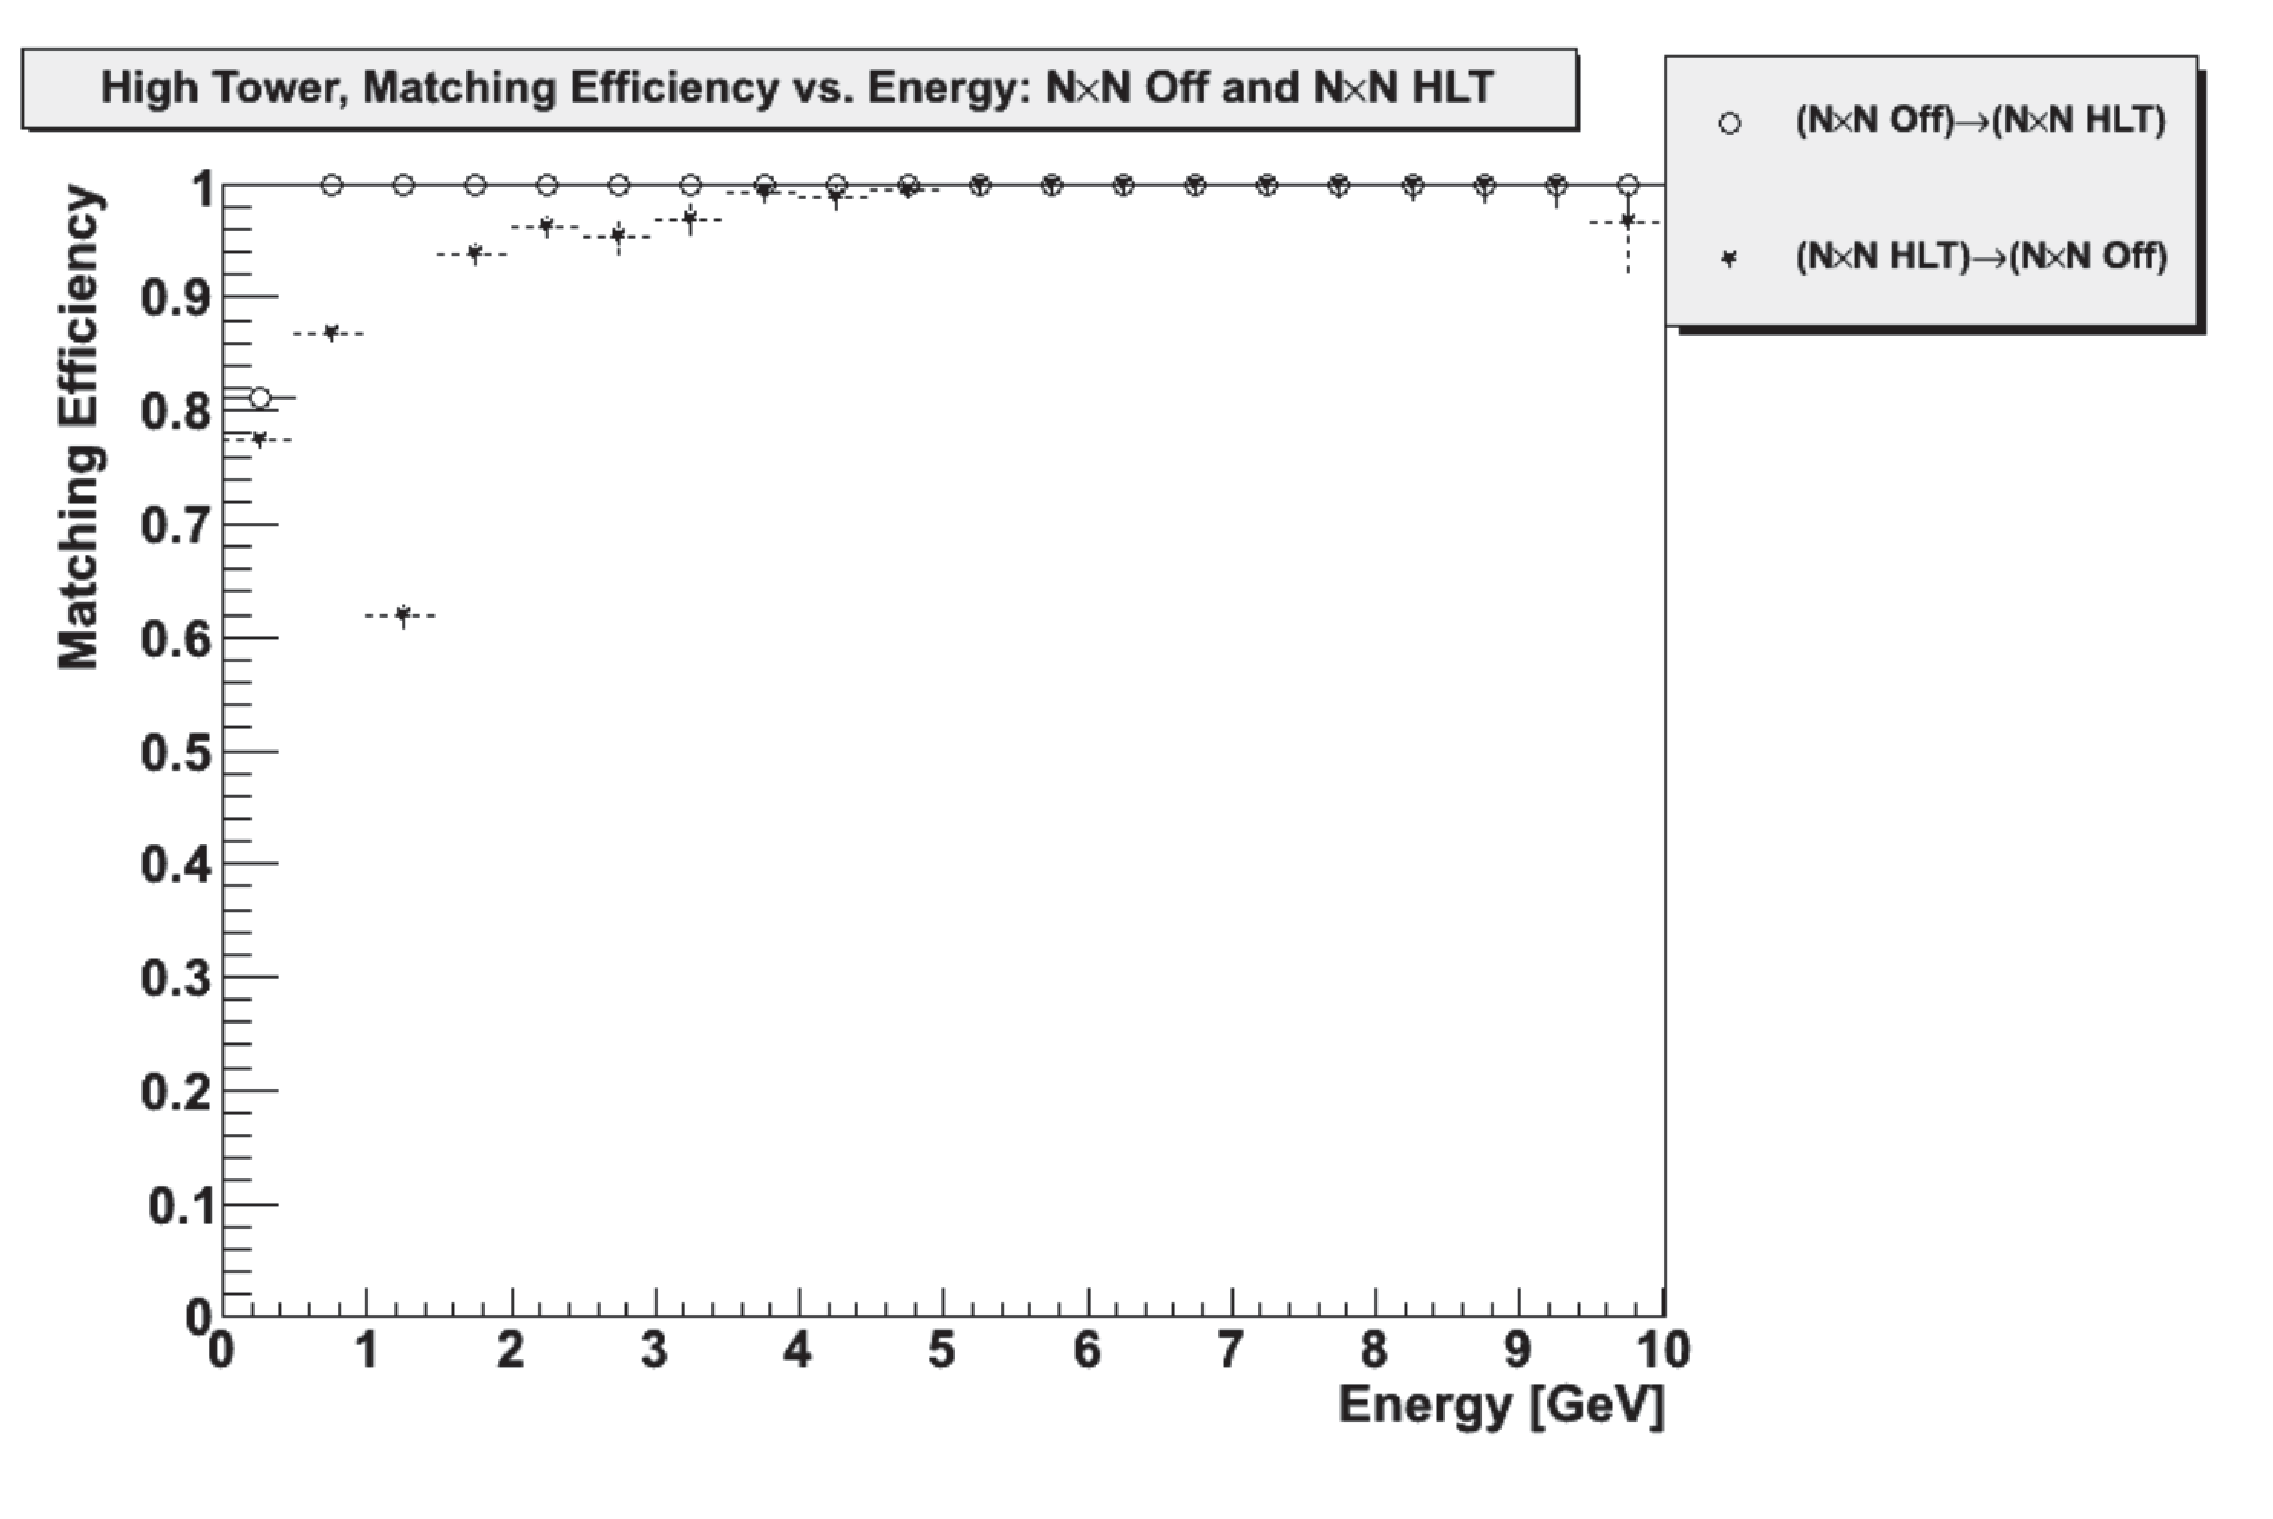
\includegraphics[width=18pc]{clus-comp.eps}
\includegraphics[width=16pc]{figures/emcal_cluster_match_nxn.pdf}
\caption{\label{f5} Reconstruction efficiency for the $N\times N$ algorithm  (cutoff) in offline and HLT. The notation $(A) \rightarrow (B)$ indicates
the fraction of clusters found using method A that are also found using method B (data from run 154787, period LHC11c).}
\end{minipage}\hspace{2pc}
\begin{minipage}{16pc}
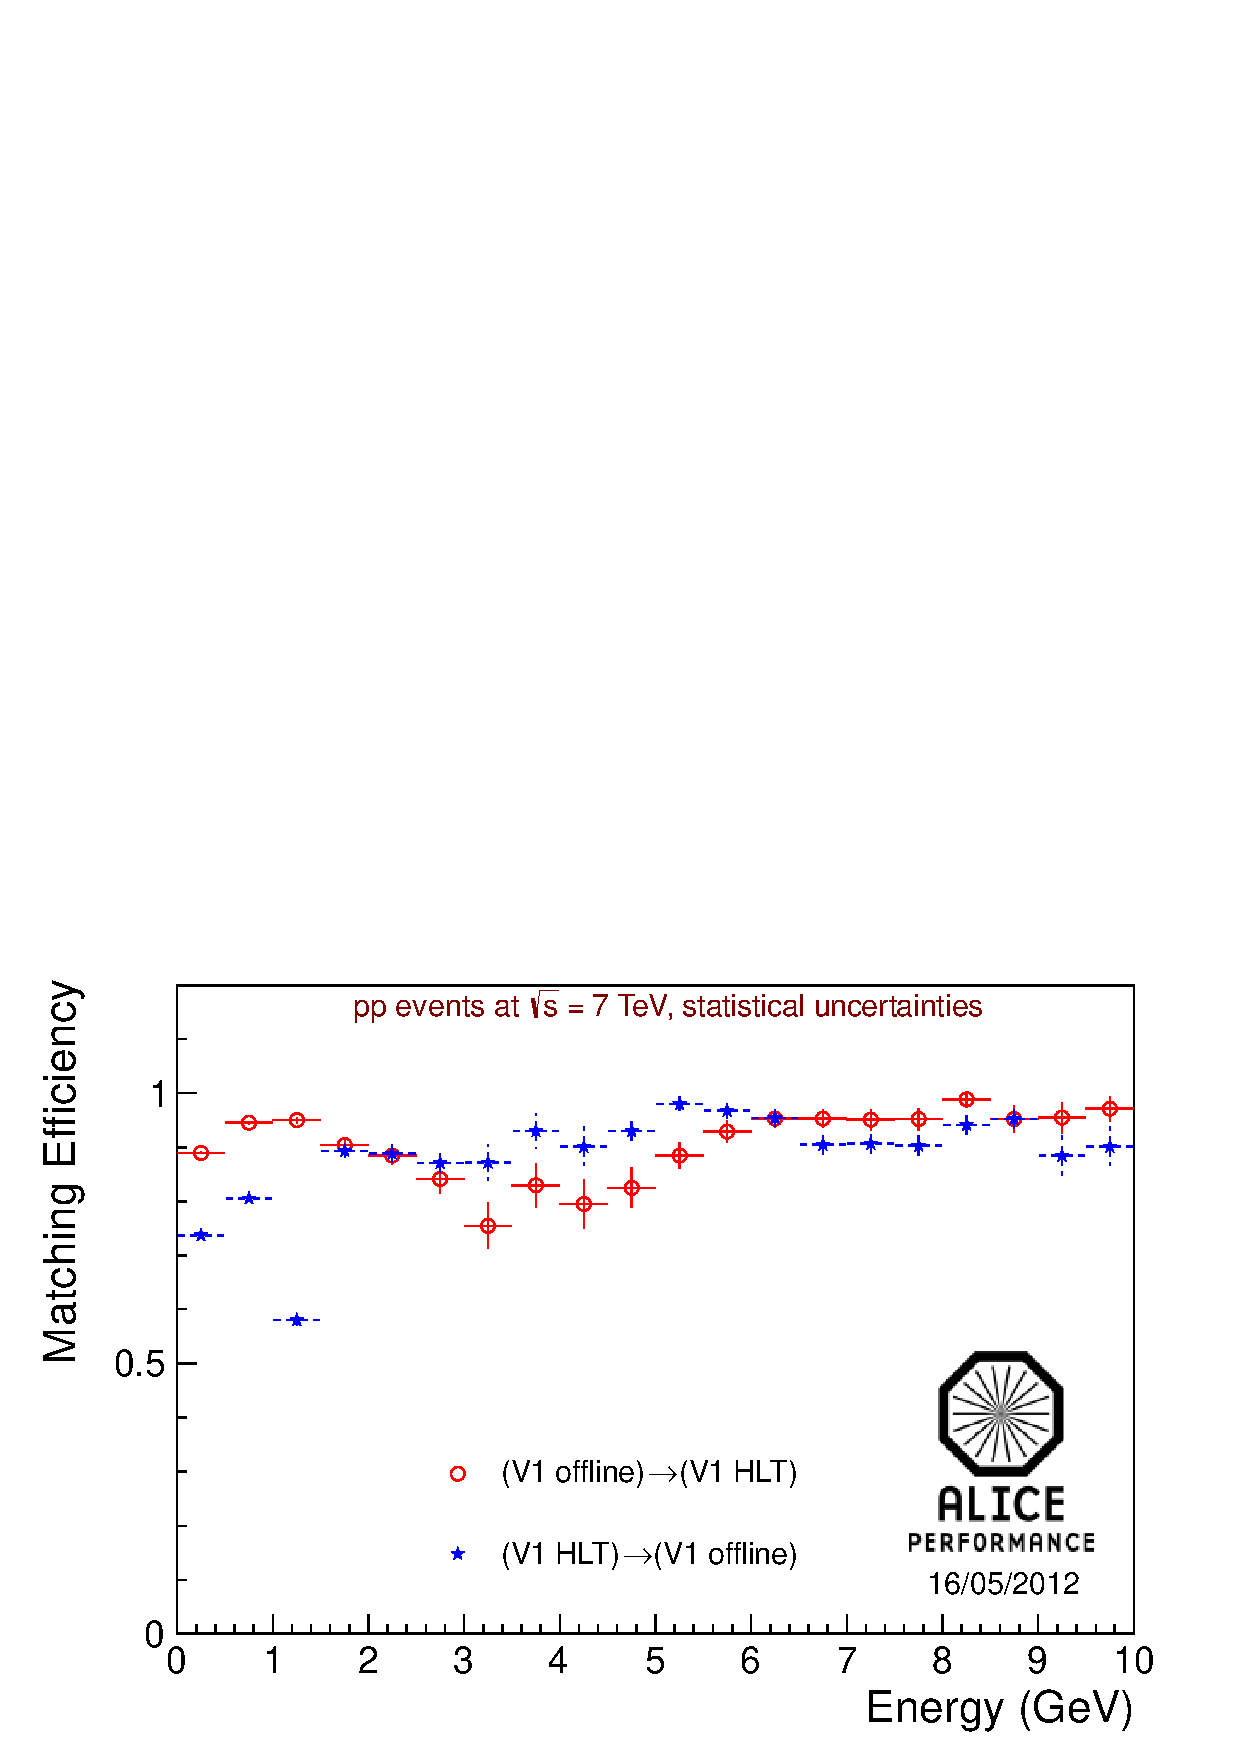
\includegraphics[width=16pc]{figures/emcal_cluster_match_v1.pdf}
\caption{\label{f6}Reconstruction efficiency for the $V1$ algorithms (no cutoff) in offline and HLT. The notation $(A) \rightarrow (B)$ indicates
the fraction of clusters found using method A that are also found using method B (data from run 154787, period LHC11c).}
\end{minipage} 
\end{figure}

The identification of an isolated single electromagnetic cluster in the EMCal can be performed using different
strategies: summing up all the neighboring cells around a seed-cell over threshold until no more cells are found 
or adding up cells around the seed until the number of clustered cells reaches the predefined cutoff value.

The first approach is more suitable for an accurate reconstruction. A further improvement to this 
clustering algorithm would be the ability to unfold overlapping clusters as generated from the 
photonic decay of high-energy neutral mesons, however this procedure usually requires computing intensive fitting algorithms. 

Such performance penalty must be avoided in the online reconstruction so the cutoff
technique is preferred.  In the EMCal HLT reconstruction a cutoff of 9 cells is used (according to the 
geometrical granularity of the single cell size), so the clusterization is performed into a 
square of $3\times3$ cells. The cutoff and non-cutoff algorithms are referred to as $N\times N$ and $V1$, respectively.

In {\it pp} collisions the response of the two methods is very similar since the majority of clusters are well separated, while  
in {\it PbPb} collisions, especially in central events, the high particle multiplicity requires the use of the cutoff (or unfolding in offline) 
to disentangle the cluster signals from the the underlying event to avoid the generation of  artificially large clusters.

The quality of the EMCal online clusterizer algorithms implemented in the HLT chain were checked against offline, 
as shown in Figures \ref{f5} and \ref{f6} where it can be seen that the performance is in a reasonable agreement in all cases.
The low point at 1.25 GeV is due to bad towers, which are assigned an energy of 1 GeV.  
%The HLT clusterizer does not have the capability to remove bad clusters.  
Bad clusters are removed in later stages of the analysis, but that is not yet reflected in Figures \ref{f5} and \ref{f6}.  
This effect leads to an excess of clusters that are found by the HLT clusterizer, but not by the offline clusterizer.\\

Since the EMCal HLT reconstruction is mainly targeted for triggering, a small penalty in the accuracy of the energy reconstruction of the clusters is accepted 
as a trade off in favor of faster performance, and for this reason the cutoff clustering method was used, especially in {\it PbPb} collisions.

\subsection{Trigger components}

The online HLT chain is capable of producing trigger decisions based on full
event reconstruction. In terms of EMCal event rejection the following relevant trigger observables
have been implemented:

\begin{itemize}
\item neutral cluster trigger
\item electron and jet trigger
\end{itemize}


\subsubsection{Cluster trigger} 
The single shower triggering mode is primarily targeted to trigger on photons and neutral mesons.
In all collision systems, the high level trigger post-filtering can improve  
the hardware L0 and L1 trigger response by using the current bad channels map information
and calibration factors (which could be recomputed directly in the HLT).

\subsubsection{Electron trigger}
For this trigger  the cluster information reconstructed online by the EMCal HLT analysis 
chain is combined with the central barrel tracking information to produce complex event selection 
as a single electron trigger (matching of one extrapolated track with an EMCal cluster.
% TCA - this shouldn't be in this section, if it is included...
%, and requiring a match between the cluster energy and the track momentum) and a full jet trigger
%(matching of multiple tracks with a jet patch in the EMCal).
Performance and accuracy studies of the track matching component developed for this purpose 
have been done using simulated and real data taken during the 2011 LHC running period. 
Results are shown in Figures \ref{f7} and \ref{f8} where the cluster - track residuals
in azimuth and pseudo-rapidity units are to be compared with a calorimeter cell size of 
$0.014\times 0.014$.

\begin{figure}[hb]
\begin{minipage}{16pc}
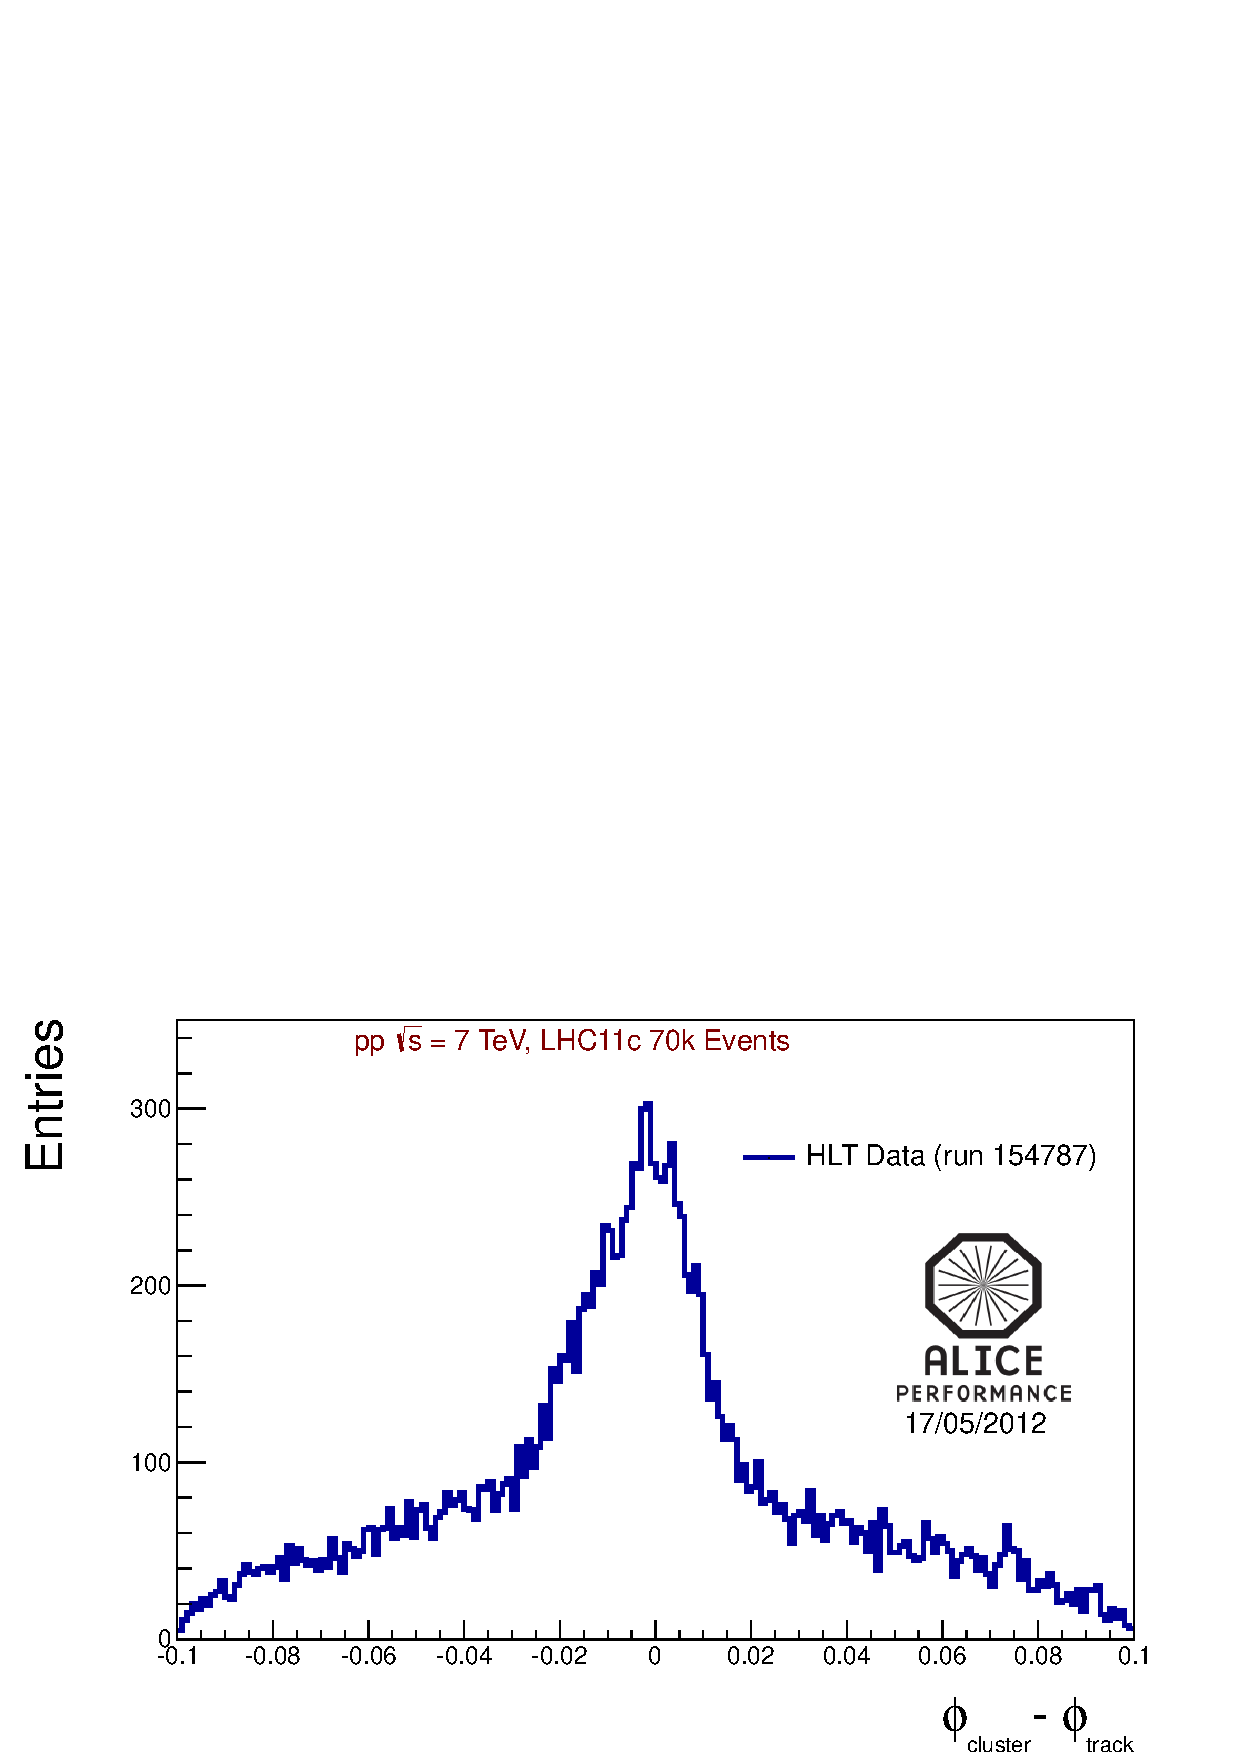
\includegraphics[width=15.5pc]{figures/Fig4dPhi_performance.pdf}
\caption{\label{f7} 
Distribution of the residuals in azimuth ($\Delta\phi$) for the EMCal cluster and central barrel tracks
obtained using the HLT online chain for run 154787 (LHC11c), ~ 70 k events reconstructed. 
}
\end{minipage}\hspace{2pc}
\begin{minipage}{16pc}
\includegraphics[width=16pc]{figures/Fig5dEta_performance.pdf}
\caption{\label{f8} 
Distribution of the residuals in pseudo-rapidity ($\Delta\eta$) for the EMCal cluster and central barrel tracks
obtained using the HLT online chain for run 154787 (LHC11c), ~ 70 k events reconstructed.
}
\end{minipage} 
\end{figure}


In addition to the extrapolation of the track from the central barrel
to the EMCal interaction plane and the matching with a compatible nearby cluster, 
the electron trigger component must finally perform particle identification 
to issue a trigger decision. The selection of electron candidates is done 
using the $E/pc$ information where the energy is measured from the
EMCal cluster and the momentum from the central barrel track.
The trigger component is initialized with default values
for the cut of $0.8< E/pc <1.3$. The default cuts are stored in the HLT
conditions database and can be overridden via command line arguments
at configuration time (usually at start of run).

The performance of the electron trigger was studied using {\it pp} minimum 
bias data at 7 TeV with embedded $J/\Psi$ events.
Figure \ref{f9} shows the good agreement of the $E/pc$ distributions 
obtained with the track extrapolation - cluster matching 
performed using the online algorithms compared to the ESD-based tracking (red).

\begin{figure}[ht]
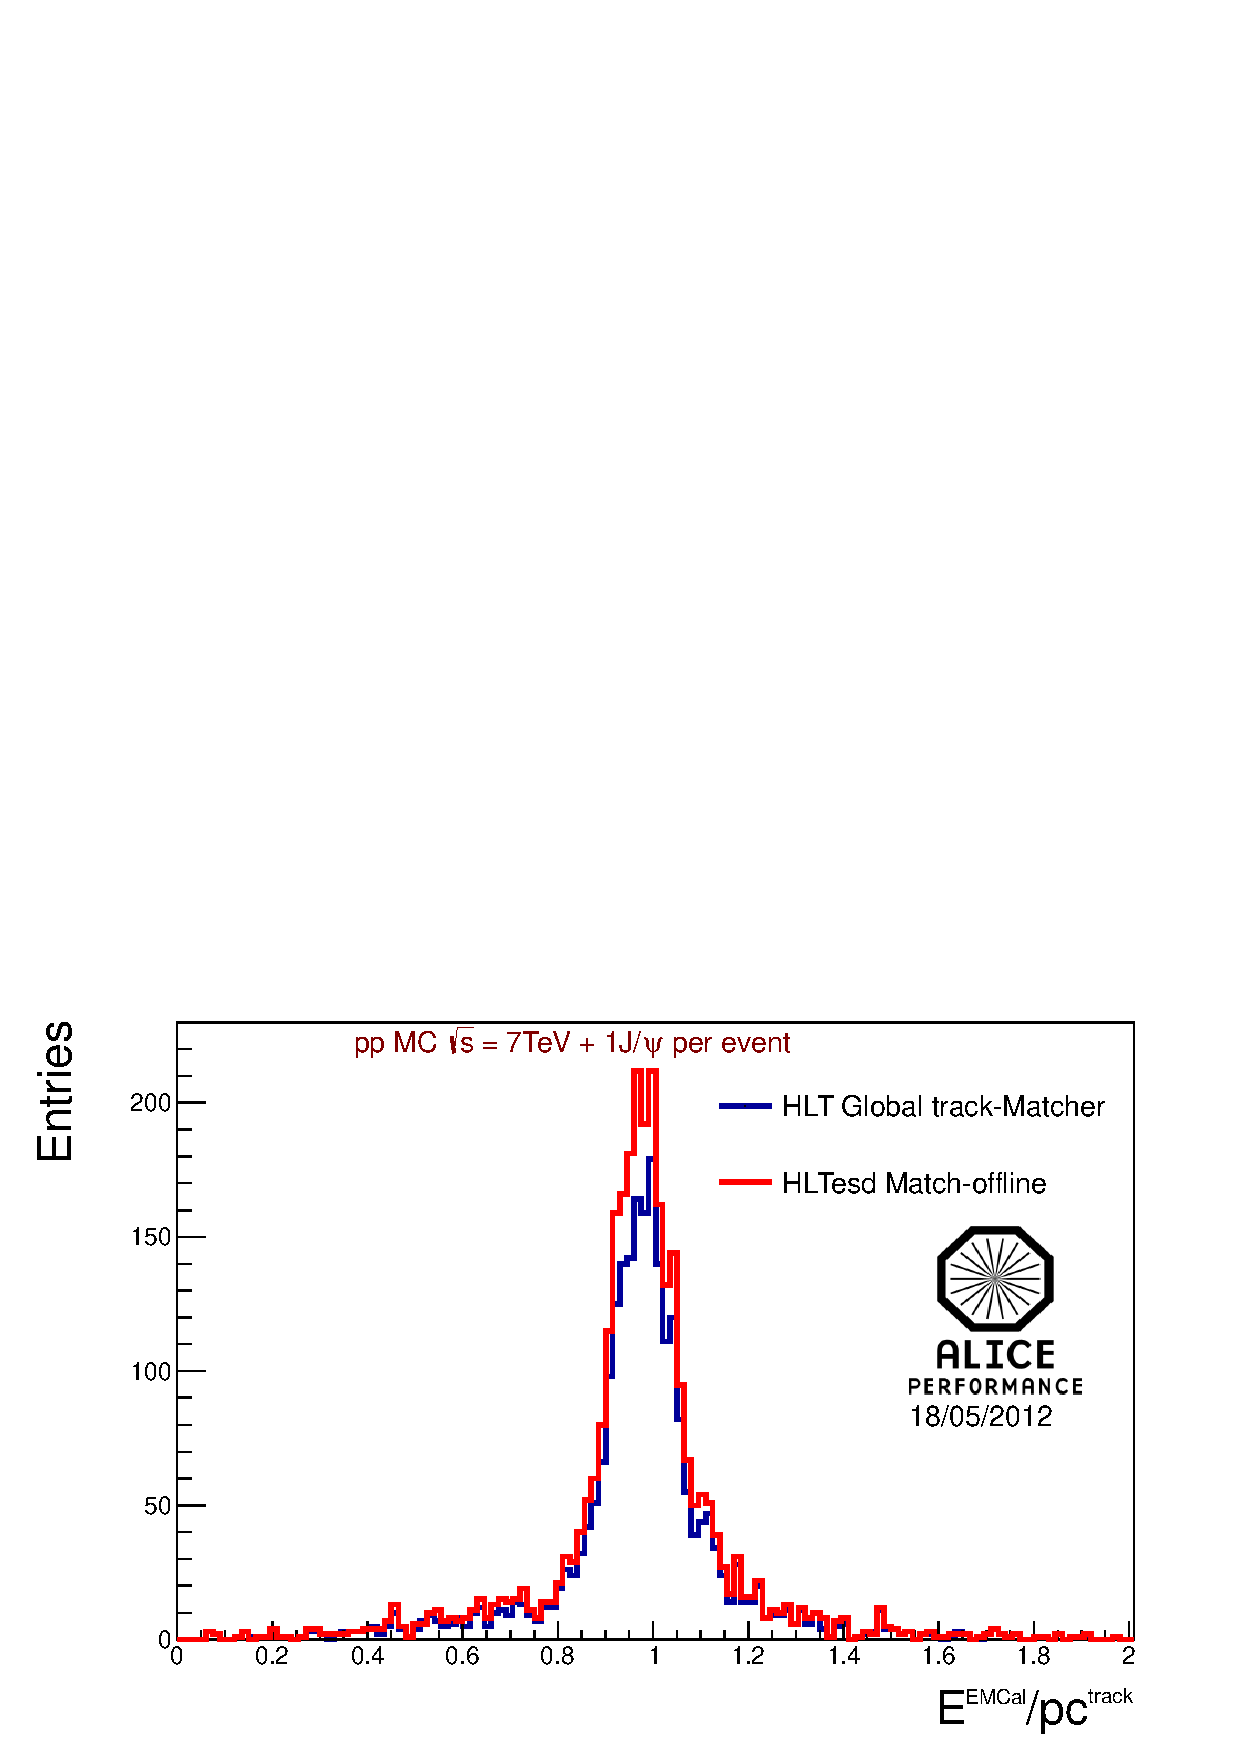
\includegraphics[width=24pc]{figures/Fig6HLTEoverP_performance.pdf}
\begin{center}
\caption{\label{f9} 
$E/pc$ distributions obtained with the track extrapolation - cluster matching
via the online algorithms compared to the ESD-based tracking (red).}
\end{center}
\end{figure}

To determine the possible improvement of the event selection 
for electrons with energies above 1~GeV, AliRoot simulations of the HLT chain using LHC11b10a {\it pp} minimum bias data 
at 2.76 GeV and the EMCal full geometry (10 super-modules)  have been used. These studies
have shown that at least a factor 5 to 10 in event selection can be gained compared to the single shower trigger, as shown in Figure \ref{f10}.

\begin{figure}[ht]
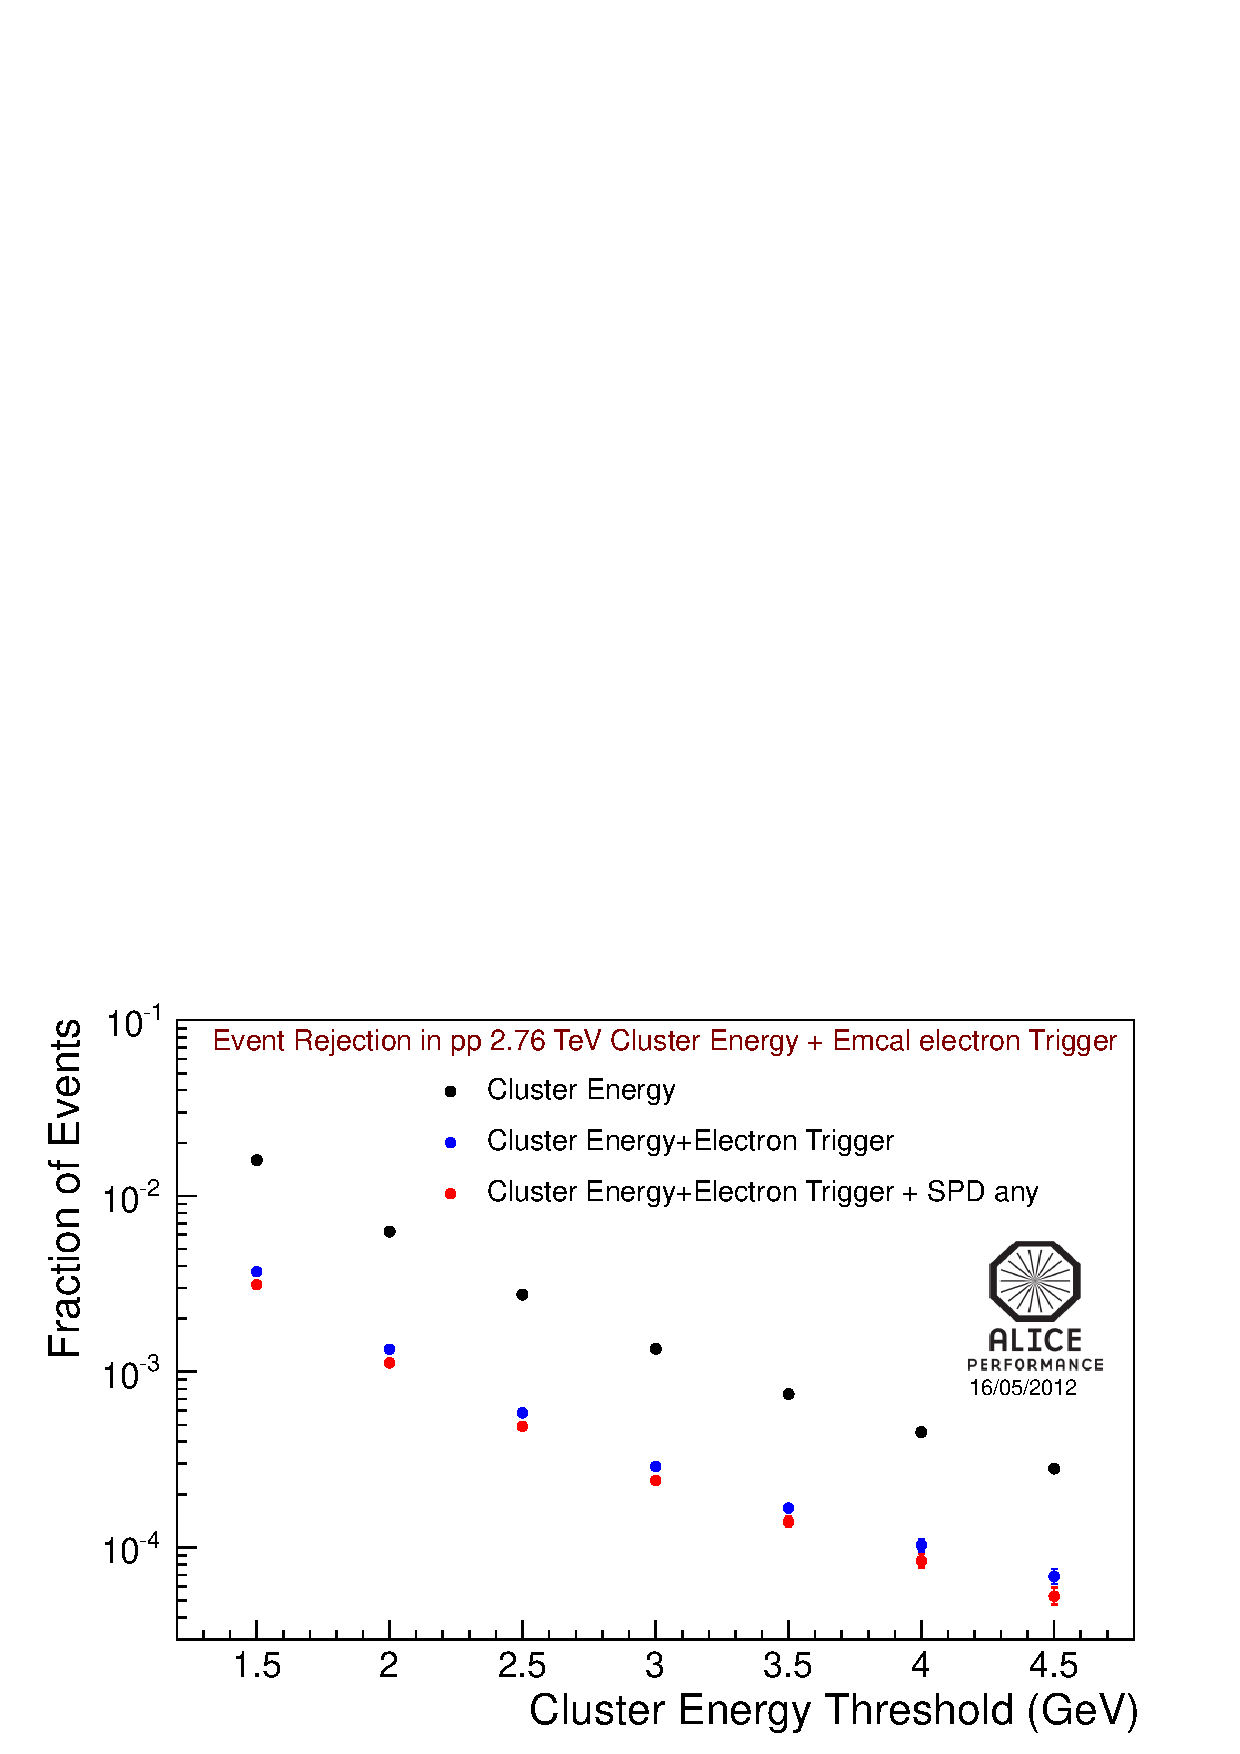
\includegraphics[width=24pc]{figures/Fig7Events_performance.pdf}
\begin{center}
\caption{\label{f10} 
Improvement in the event selection for $E_{e^-}>$~1~GeV from AliRoot simulation (anchor to LHC11b10a) with minimum bias {\it pp} at $\sqrt{s}=2.76$~TeV (EMCal full geometry).
The red points are obtained with the requirement of one hit in one of the silicon pixel (SPD) layers to reject a higher fraction of photon conversions.
}
\end{center}
\end{figure}


\subsubsection{Jet trigger}

The EMCal online jet trigger component was developed to provide 
an unbiased jet sample by refining the hardware L1 trigger decisions.
In fact, the HLT post-processing can produce a sharper turn on curve 
using the track matching capabilities of the online reconstruction chain. 
In addition, a more accurate definition of the jet area than the one provided by the hardware L1 jet patch, 
can be obtained choosing a jet cone based on the jet direction calculated online.
The combination of the hadronic and electromagnetic energy provides a measurement of 
the total energy of the jet by matching the tracks identified as part of the jet with 
the corresponding EMCal neutral energy.

The use of the HLT jet trigger also allows a better characterization 
of the trigger response as a function of the centrality dependent threshold 
by re-processing the information from the V0 detector directly in HLT.

Performance considerations, due to the high particle multiplicity    
in {\it PbPb} collisions, impose that the track extrapolation is done only geometrically
without taking into account  multiple scattering effects
introduced by the material budget in front of the EMCal. 
The pure geometrical extrapolation accounts for a speedup factor of 20 in the
execution of the track matcher component with respect to the 
full-fledged track extrapolation used in {\it pp} collisions.

The identification of the jet tracks is performed using the anti-$k_T$ 
jet finder provided by the FastJet package.

The EMCal jet trigger was only partially tested during the 2011 data taking period
and will be fully commissioned for the LHC {\it pPb} run period in 2012.

\subsection{Monitoring components}

The role of the EMCal HLT reconstruction in {\it pp} collisions is targeted mainly on 
the monitoring functions since the expected event sizes are small enough for 
the complete collision event to be fully transferred to permanent storage. 
\begin{figure}[h]
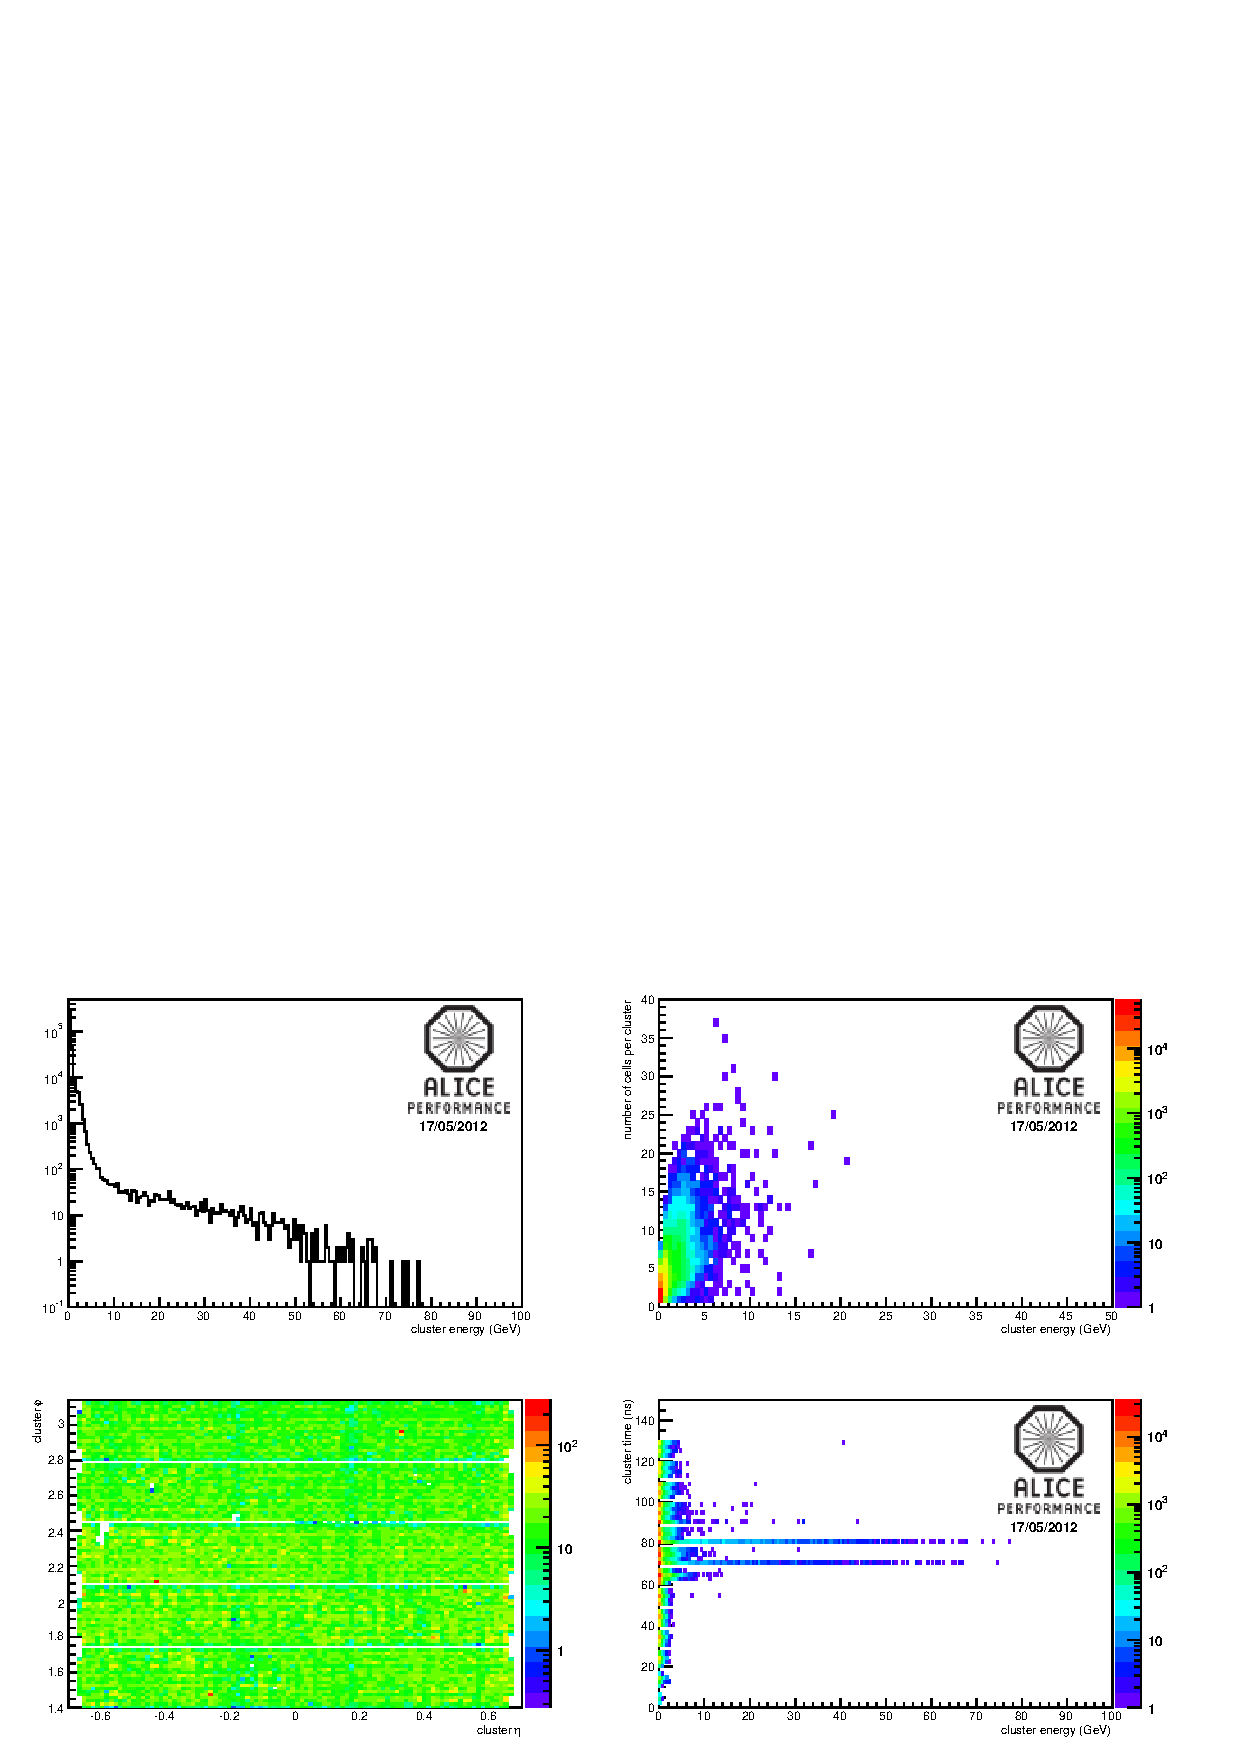
\includegraphics[width=26pc]{figures/all-monitor.pdf}
\begin{center}
\caption{\label{f2} Output from the EMCal HLT monitoring component. Top left: cluster energy spectra as a function of the  reconstructed cluster energy; 
bottom left: cluster position in  $\eta$ and $\phi$ coordinates; bottom right: cluster time distribution; top right: number of cells per cluster vs cluster 
energy. LHC11b period, $\sqrt{s}=7$ TeV {\it pp} data, 10~kEvent analyzed.}
\end{center}
\end{figure}

In this respect, two monitoring components have been developed and deployed in the online chain.
The first component currently monitors reconstructed quantities, such as the cluster energy spectra and timing, 
the cluster position in the $\eta$ and $\phi$ coordinates, and the number of cells per cluster 
as a function of the cluster reconstructed energy as shown in Figure \ref{f2}.

\begin{figure}[h]
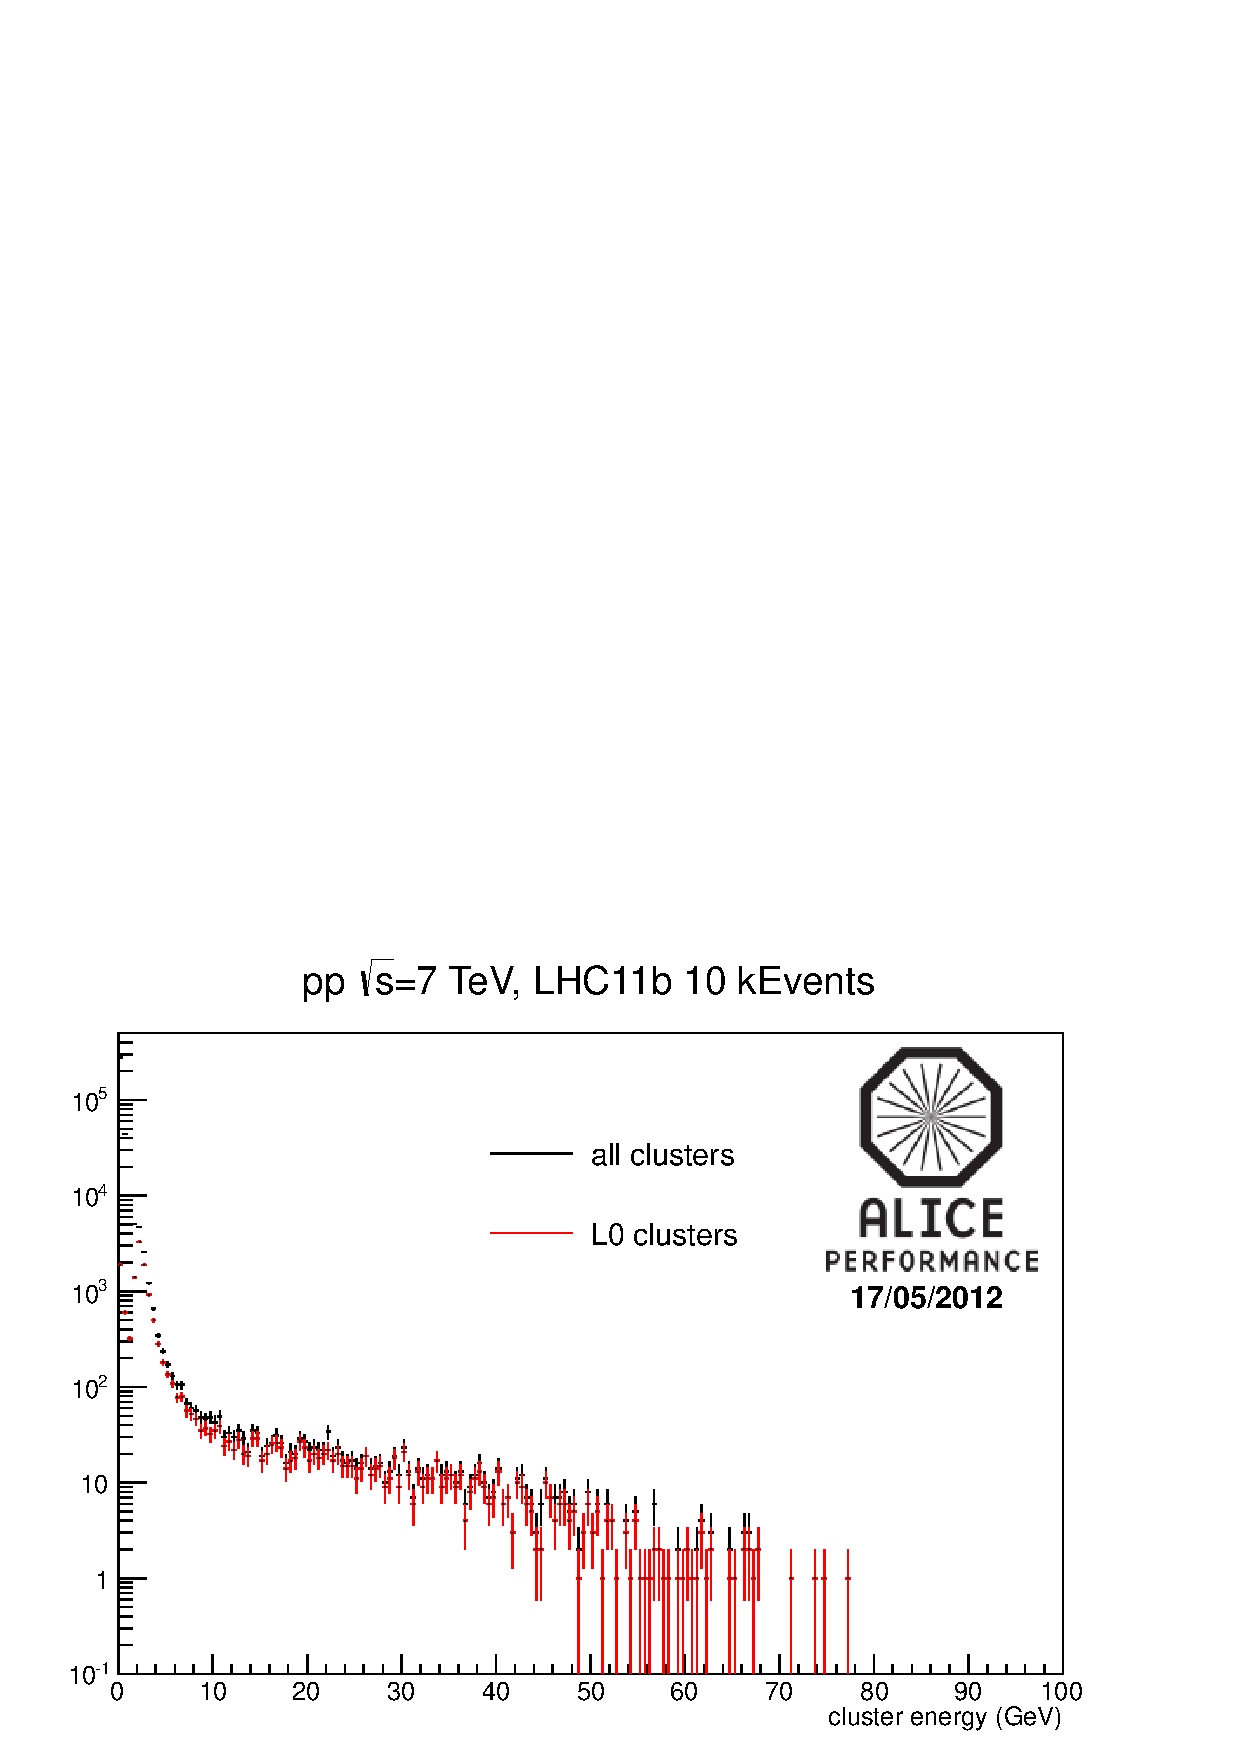
\includegraphics[width=24pc]{figures/l0clusters.pdf}
\begin{center}
\caption{\label{f3} Energy spectrum for all clusters reconstructed by the EMCal (black points) superposed with the triggered cluster spectrum
(i.e. clusters reconstructed which also carry the L0 hardware trigger bit set, red points). }
\end{center} 
\end{figure}

The second component re-evaluates the EMCal hardware trigger decisions by recalculating
the cluster energy spectrum for all the clusters with the L0 trigger bit set as shown 
in Figure \ref{f3}. The L0 turn on curve can then be calculated online as the ratio between
the triggered and the reconstructed cluster spectra and monitored for the specific run.


No recalculation of hardware L1 trigger primitives was possible
during the 2011 data taking since the optical link from the EMCal L1 trigger unit 
could only installed during the 2011-2012 winter shutdown of the LHC hence
the software development for the L1 trigger monitoring is still underway.



Documented in \cite{EMCAL:HLT}. Add Summary or more info here.
\clearpage

\section{Analysis format and code}

All the reconstructed particles of all the detectors are kept
in a file called \textbf{AliESDs.root}. The detectors must store there
the most relevant information which will be used in the analysis. 
Together with the AliESDs.root file, another file is created with some reference tags of the simulated events, containing for example the number of events per run. This file is
named \textbf{Run0.Event0\_1.ESD.tag.root} (1 means that only 1 event
was simulated). 

In order to do the analysis with the data contained in the ESDs, the only file needed is \textbf{AliESDs.root} in the local directories or a grid collection. No other files are needed in the working directory (such as galice.root nor EMCAL.{*}.root) unless one needs to access the primary particles generated during the simulation. In that case, the files \textbf{galice.root} and \textbf{Kinematics.root} are needed locally.  Also, if one want to access to some information of the detector geometry, the \textbf{geometry.root} file is needed.

There are other data analysis containers created from the ESD, the
AOD (Analysis Object Data) with smaller quantity of data for most of the subsystems but for the calorimeters, where we copy all the information\footnote{until half 2012 everything but the time of the cells was stored}.


\subsection{Calorimeter information in ESDs/AODs}

The basic calorimeter information needed for analysis is stored in the ESDs or AODs in the form of CaloClusters and CaloCells (cell = EMCal Tower or PHOS crystal). Also there is some information stored in the AOD/ESD event classes, it will be detailed more in the lines below. Both AOD and ESD classes derive from virtual classes so that with a similar analysis code and access methods, we can read both kind of data formats.


\subsubsection{AliVEvent (AliESDEvent, AliAODEvent)}

Those are manager classes for the event information retrieval. Regarding the calorimeters they have the following access information (getters) methods\footnote{There are the equivalent setters just have a look to the header file of the class}:
\begin{itemize}

\item AliVCaloCluster *GetCaloCluster(Int\_t i) : Returns a CaloCluster listed in position "i" in the array of CaloClusters. It can be either PHOS or EMCal (PHOS list of clusters is before the EMCal list).

\item TClonesArray *GetCaloClusters() :  Returns the array with CaloClusters PHOS+EMCAL, Only defined for AODs

\item Int\_t GetEMCALClusters(TRefArray *clusters) ; Int\_t GetPHOSClusters(TRefArray *clusters) : Returns an array with only EMCal clusters or only with PHOS clusters.

\item Int\_t GetNumberOfCaloClusters(): Returns the total number of clusters PHOS+EMCAL.

\item AliVCaloCells *GetEMCALCells();  AliESDCaloCells *GetPHOSCells() : Returns the pointer with the CaloCells object for EMCal or PHOS.

\item AliVCaloTrigger *GetCaloTrigger(TString calo) : Access to trigger patch information, for calo="PHOS" or calo="EMCAL"

\item const TGeoHMatrix* GetPHOSMatrix(Int\_t i); const TGeoHMatrix* GetEMCALMatrix(Int\_t i): Get the matrices for the transformation of global to local. The transformation matrices are not stored in the AODs.



\end{itemize}



\subsubsection{AliVCaloCluster (AliESDCaloCluster,AliAODCaloCluster)}

They  contain the information of the calorimeter clusters. Note that PHOS and EMCAL CaloClusters are kept in the same TClonesArray (see above). The information stored in each CaloCluster is :

\begin{itemize}
\item General
	\begin{itemize}
	\item Int\_t GetID(): It returns a unique identifier number for a CaloCluster.

	\item Char\_t GetClusterType():It returns kPHOSNeutral (kPHOSCharged exists but not used) or  kEMCALClusterv1. Another way to get the origin of the cluster:

	\item Bool\_t IsEMCAL(); Bool\_t IsPHOS(). 

	\item void GetPosition(Float\_t *pos) : It returns a {x,y,z} array with the global positions of the clusters in centimeters.

	\item Double\_t E() : It returns the energy of the cluster in GeV units.

	\item void GetMomentum(TLorentzVector\& p, Double\_t * vertexPosition ): It fills a TLorentzVector pointing to the measured vertex of the collision. It also modifies the cluster global positions to have a vector pointing to the vertex, this has to be corrected. Assumes that cluster is neutral. To be used only for analysis with clusters not matched with tracks.
	\end{itemize}
\item Shower Shape
	\begin{itemize}

	\item Double\_t GetDispersion(): Dispersion of the shower.

	\item Double\_t Chi2(): Not filled.

	\item Double\_t GetM20()  Double\_t GetM02() : Ellipse axis.

	\item UChar\_t GetNExMax() : Number or maxima in cluster. Not filled.

	\item Double\_t *GetPID(): PID weights array, 10 entries corresponding to the ones defined in AliPID.h

	 \item enum EParticleType { kElectron = 0,  kMuon = 1, kPion = 2, kKaon = 3, kProton = 4, kPhoton = 5, kPi0 = 6, kNeutron =7, kKaon0 = 8, kEleCon = 9,kUnknown = 10}; : PID tag numbers, corresponding to the PID array

	\item Double\_t GetDistanceToBadChannel() : Distance of the cluster to closest channel declared as kDead, kWarm or kHot.

	\item Double\_t GetTOF() :  Measured Time of Flight of the cluster.
	\end{itemize}

\item Track-Cluster matching
	\begin{itemize}

	\item TArrayI * GetTracksMatched(): List of indexes to the likely matched tracks. Tracks ordered in matching likeliness. If there is no match at all, by default it contains one entry with value -1. Only in ESDs.

	\item Int\_t GetTrackMatchedIndex(Int\_t i): Index of track in position "i" in the list of indices stored in GetTracksMatched(). Only in ESDs

	\item Int\_t GetNTracksMatched() : Total number of likely matched tracks. Size of GetTracksMatched() array.

	\item Double\_t GetEmcCpvDistance() : PHOS method, not used anymore. Use instead those below.

	\item Double\_t GetTrackDx(void), Double\_t GetTrackDz(void): Distance in x and z to closest track. 

	\item TObject * GetTrackMatched(Int\_t i): References to the list of most likely matched tracks are stored in a TRefArray. This method retrives the one in position "i". Tracks are listed in order of likeliness. The TObject is a AliAODTrack. Only for AODs

	\end{itemize}

\item MonteCarlo labels:
	\begin{itemize}

	\item TArrayI * GetLabels(): List of indexes to the MonteCarlo particles that contribute to the cluster. Labels ordered in energy contribution.

	\item Int\_t GetLabel(): Index of MonteCarlo particle that deposited more energy in the cluster. First entry of GetLabels() array.
	
         \item Int\_t GetLabelAt(UInt\_t i): Index of MonteCarlo particle in position i of the array of MonteCarlo indices.

	\item Int\_t GetNLabels() : Total number of MonteCarlo particles that deposited energy. Size of GetLabels() array.
	\end{itemize}

\item Cluster cells
	\begin{itemize}

	\item Int\_t GetNCells() : It returns the number of cells that contribute to the cluster.

	\item UShort\_t *GetCellsAbsId(): It returns the array with absolute id number of the cells contributing to the cluster. Size of the array is given by GetNCells().

	\item Double32\_t *GetCellsAmplitudeFraction(): For cluster unfolding, it returns an array with the fraction the energy that a cell contributes to the cluster. 

	\item Int\_t GetCellAbsId(Int\_t i) : It returns the absolute Id number of a cell in the array between 0 and GetNCells()-1. 

	\item Double\_t GetCellAmplitudeFraction(Int\_t i) : It returns the amplitude fraction of a cell in the array between 0 and GetNCells()-1.

	\end{itemize}

 \end{itemize}


\subsubsection{AliVCaloCells (AliESDCaloCells, AliAODCaloCells)}
They   contain an array with  the amplitude or time of all the cells that fired in the calorimeter during the event. Notice that per event there will be a CaloCell object with EMCAL cells and another one with PHOS cells.

\begin{itemize}

	\item Short\_t GetNumberOfCells(): Returns number of cells with some energy.
	
	\item Bool\_t IsEMCAL(); Bool\_t IsPHOS(); Char\_t  GetType(): Methods to check the origin of the AliESDCaloCell object, kEMCALCell or kPHOSCell.

	\item Short\_t  GetCellNumber(Short\_t pos):  Given the position in the array of cells (from 0 to GetNumberOfCells()-1), it returns the absolute cell number (from 0 to NModules*NRows*NColumns - 1).

	\item Double\_t GetCellAmplitude(Short\_t cellNumber): Given absolute cell number of a cell (from 0 to NModules*NRows*NColumns - 1), it returns the measured amplitude of the cell in GeV units.

	\item Double\_t GetCellTime(Short\_t cellNumber):  Given absolute cell number of a cell (from 0 to NModules*NRows*NColumns - 1), it returns the measured time of the cell in second units.

	\item Double\_t GetAmplitude(Short\_t pos): Given the position in the array of cells (from 0 to GetNumberOfCells()-1), it returns the amplitude of the cell in GeV units. 

	\item Double\_t GetTime(Short\_t pos):  Given the position in the array of cells (from 0 to GetNumberOfCells()-1), it returns the time of the cell in second units. 

	\item Double\_t GetCellMCLable(Short\_t cellNumber): Given absolute cell number of a cell (from 0 to NModules*NRows*NColumns - 1), it returns the index of the most likely MC label.

	\item Double\_t GetCellEFraction(Short\_t cellNumber):  Given absolute cell number of a cell (from 0 to NModules*NRows*NColumns - 1), it returns the fraction of embedded energy from MC to real data (only for embedding)

	\item  Double\_t GetMCLabel(Short\_t pos): Given the position in the array of cells (from 0 to GetNumberOfCells()-1), it returns the index of the most likely MC label.

	\item Double\_t GetEFraction(Short\_t pos):  Given the position in the array of cells (from 0 to GetNumberOfCells()-1), it returns the fraction of embedded energy from MC to real data (only for embbedding)

          \item Bool\_t   GetCell(Short\_t pos, Short\_t \&cellNumber, Double\_t \&amplitude, Double\_t \&time, Short\_t \&mclabel,    Double\_t  \&efrac); : For a given position of the list of cells, it fills the amplitude, time, mc lable and fraction of energy.
          
          
 \end{itemize}

\subsubsection{AliVCaloTrigger (AliESDCaloTrigger, AliAODCaloTrigger) - Rachid)}

\subsection{Macros}
You can find example macros to run on ESDs or AODs in 
\begin{lstlisting}
$ALICE_ROOT/EMCAL/macros/TestESD.C or TestAOD.C
\end{lstlisting}

 All the ESDs information is filled via the AliEMCALReconstructor/AliPHOSReconstructor class, in the method FillESD(). The AODs are created via the analysis class 

\begin{lstlisting}
$ALICE_ROOT/ANALYSIS/AliAnalysisTaskESDfilter.cxx,.h
\end{lstlisting}

and as already mentioned, for the calorimeters it basically just copies all the information from ESD format to AOD format. 

Below is a description of what information is stored and how to retrieve it. The location of the corresponding classes is
\begin{lstlisting}
$ALICE_ROOT/STEER
\end{lstlisting}



\subsection{Code example}

The analysis is done using the data stored in the ESD. The macro
\begin{lstlisting}
$ALICE_ROOT/EMCAL/macros/TestESD.C
\end{lstlisting}
is an example of how to read the data for the calorimeters PHOS and
EMCal (just replace where it says EMCAL by PHOS in the macro to obtain
PHOS data). For these detectors we have to use the ESD class AliESDCaloCluster or AliESDCaloCells to retrieve all the calorimeters information. For the tracking detectors,
the class is called AliESDtrack, but the way to use it is very similar
(see ``\$ALICE\_ROOT/STEER/AliESDtrack.*''\\ and ``\$ALICE\_ROOT/STEER/AliESDCaloCluster*'' for more details). In AliESDCaloCluster we keep the following
cluster information: energy, position, number of Digits that belong
to the cluster, list of the cluster Digits indeces, shower dispersion, shower lateral axis and a few more parameters. In AliESDCaloCells we keep the following
tower information: amplitude (GeV), time (seconds), absolute cell number.

The structure of the ESD testing macro (TestESD.C) is the
following:

\begin{itemize}
\item Lines 0-29: This macro is prepared to be compiled so it has ``includes'' to all the Root and AliRoot classes used.

\item Lines 30-36: This macro prints some information on screen, the kind of information is set here. We  print by default clusters information and optionally, the cells information, the matches information, the cells in the clusters information or the MonteCarlo original particle kinematics.

\item Lines 40-64: Here are the methods used to load AliESDs.root , geometry or kinematics files. Also loop on ESD event is here.

\item Lines 65-66 Gets the measured vertex of the collision.

\item Lines 69-78 Loops on all the CaloCell entries and prints the cell amplitude, absolute number and time.
 
\item Lines 84- end:  We access the  EMCAL AliESDCaloCluster  array and loop on it. 
We get the different information from the CaloCluster.

\item Lines 111-130:  Track Matching prints. Access to the matched track stored in AliESDtrack.

\item Lines 133-159: Cells in cluster prints

\item Lines  161 - end: Access the stack with the MC information and prints the parameters of the particle that generated the cluster.


\end{itemize}

\subsection{Advanced utilities : Reconstruction/corrrections of cells, clusters  during the analysis}

\subsubsection{AliEMCALRecoUtils}
\subsubsection{Tender : AliEMCALTenderSupply}

\subsubsection{Particle Identification with the EMCal}

In the EMCal we have two different ways to obtain the PID of a given particle:
\begin{enumerate}
\item Shower shape of the cluster: Distinguish electrons/photons and $\pi^{0}$ from other particles. This is done without any track information in the class \texttt{AliEMCALPID}.
\item Ratio between energy of the cluster and the momentum of a matched track: Distinguish electrons from other particles. This is done in the combined PID framework by the class \texttt{AliEMCalPIDResponse}.
\end{enumerate}

\paragraph{AliEMCALPID (AliEMCALPIDutils)}

The idea for particle identification with EMCal clusters is that the shower shapes produced in the EMCal are different for different particle species. The long axis of the cluster ($\lambda_{0}$) is used for this purpose and parametrized for electrons/photons (should have the same electromagnetic shower), for $\pi^{0}$ (two photons merging in one cluster give a different shape than one photon), and hadrons (MIP signal).

The main method in this class is \texttt{RunPID()}, which calls \texttt{AliEMCALPIDutils::ComputePID(Double\_t energy, Double\_t lambda0)} for each cluster with cluster energy \texttt{energy} and long axis of the cluster \texttt{lambda0} in the event. Inside this method first the \texttt{energy} dependent parametrizations for the three cases (photons, $\pi^{0}$, and hadrons) are retrieved. The parametrization is done here with a combination of a Gaussian and a Landau (at the moment there are two parameter sets available: low and high flux, which can be set by \texttt{AliEMCALPID::SetLowFluxParam()} and  \texttt{AliEMCALPID::SetHighFluxParam()}). Then a conditional probability is assigned to the cluster for each of these three species depending on \texttt{lambda0}. Finally a probability for a cluster being of a certain particle species is calculated with the Bayesian approach that can be retrieved by \texttt{AliVCluster::GetPID()}.\\
\begin{DDbox}{\linewidth}
\begin{lstlisting}
  // compute PID weights
  if( (fProbGamma + fProbPiZero + fProbHadron)>0.){
    fPIDWeight[0] = fProbGamma / (fProbGamma + fProbPiZero + fProbHadron);    // gamma
    fPIDWeight[1] = fProbPiZero / (fProbGamma+fProbPiZero+fProbHadron);          // pi0
    fPIDWeight[2] = fProbHadron / (fProbGamma+fProbPiZero+fProbHadron);        // hadron
  }
...
  //default particles
  fPIDFinal[AliPID::kElectron]  = fPIDWeight[0]/2; // electron
  fPIDFinal[AliPID::kMuon]      = fPIDWeight[2]/8;
  fPIDFinal[AliPID::kPion]      = fPIDWeight[2]/8;
  fPIDFinal[AliPID::kKaon]      = fPIDWeight[2]/8;
  fPIDFinal[AliPID::kProton]    = fPIDWeight[2]/8;
  //light nuclei
  fPIDFinal[AliPID::kDeuteron]  = 0;
  fPIDFinal[AliPID::kTriton]    = 0;
  fPIDFinal[AliPID::kHe3]       = 0;
  fPIDFinal[AliPID::kAlpha]     = 0;
  //neutral particles
  fPIDFinal[AliPID::kPhoton]    = fPIDWeight[0]/2; // photon
  fPIDFinal[AliPID::kPi0]       = fPIDWeight[1]  ; // pi0
  fPIDFinal[AliPID::kNeutron]   = fPIDWeight[2]/8;
  fPIDFinal[AliPID::kKaon0]     = fPIDWeight[2]/8;
  fPIDFinal[AliPID::kEleCon]    = fPIDWeight[2]/8;
  //
  fPIDFinal[AliPID::kUnknown]   = fPIDWeight[2]/8;
\end{lstlisting}
\end{DDbox}





\paragraph{AliEMCalPIDResponse}

The idea for particle identification with EMCal clusters AND the track information is that electrons are loosing their total energy in an electromagnetic shower inside the EMCal whereas all other charged particles only part of it. The main observable is $E/p$ with the energy of the EMCal cluster ($E$) and the momentum of a matched track ($p$). This ratio is $E/p\sim1$ for electrons and $E/p< 1$ for other charged particles. 

The decision about a particle species is done within the PID framework provided by ALICE. The main classes are: \texttt{STEER/STEERBase/AliPIDCombined} and \texttt{STEER/STEERBase/AliPIDResponse}. There are two methods of usage:
\begin{enumerate}
\item $n\sigma$ method: For each detector the multiples of $\sigma$ values are given for the deviation from the expected mean value at a given $p_{\mathrm{T}}$ (assuming a Gaussian distribution). This can be done via: \texttt{AliPIDResponse::GetNumberOfSigmas(EDetector detCode, const AliVParticle *track, AliPID::EParticleType type)}
\item Bayesian approach: In \texttt{AliPIDCombined::ComputeProbabilities(const AliVTrack *track, const AliPIDResponse *response, Double\_t* bayesProbabilities)} for each detector (included in the analysis via\\ \texttt{AliPIDCombined::SetDetectorMask(AliPIDResponse::EDetector)}) the conditional probability for the respective detector observable is calculated for each particle species (selected via\\ \texttt{AliPIDCombined::SetSelectedSpecies(AliPID::EParticleType)}). Then the probability for a track being of a certain particle type is calculated with the Bayesian approach. The initial particle abundances (priors) can be activated via\\ \texttt{AliPIDCombined::SetEnablePriors(kTRUE)} and either own priors can be loaded\\ (\texttt{AliPIDCombined::SetPriorDistribution(AliPID::EParticleType type,TH1F *prior)}) or default ones can be chosen (\texttt{AliPIDCombined::SetDefaultTPCPriors()}).
\end{enumerate}

For the case of the EMCal the $n\sigma$ as well as the conditional probability are calculated in\\ \texttt{AliEMCALPIDResponse::GetNumberOfSigmas( Float\_t pt,  Float\_t eop, AliPID::EParticleType n,  Int\_t charge)} and\\
\texttt{AliEMCALPIDResponse::ComputeEMCALProbability(Int\_t nSpecies, Float\_t pt, Float\_t eop, Int\_t charge, Double\_t *pEMCAL)}, respectively. These methods are called from \texttt{AliPIDCombined} and \texttt{AliPIDResponse} internally, so usually the user does not use them. 

To calculate $n\sigma$ and the conditional probability a parametrization of $E/p$ for the different particle species at different momenta is needed. This was retrieved from data in a clean PID sample with the help of $V0$ decays for electrons, pions and protons ($\gamma\rightarrow e^+e^-$, $K^0\rightarrow \pi^+\pi^-$, and $\Lambda\rightarrow p+\pi^-/\bar{p}+\pi^+$ ) for different periods. Electrons are parametrized with a Gaussian distribution (mean value and $\sigma$), all other particles are parametrized with a Gaussian for $0.5 < E/p < 1.5$ and the probabilty to have a value in this $E/p$ interval (this is small, since the maximum of the distribution lies around $0.1$). Here we distinguish between protons, antiprotons (higher probabilty for higher $E/p$ values due to annihilation) and other particles (pions are used for these). At the moment this parametrization is not done for all periods so far, as default LHC11d is taken. There might be especially some centrality dependence on the $E/p$ parametrization (because of the different multiplicities of track--cluster matches).

In addition to that the purity of the electron identification can be enhanced by using shower shape cuts in addition. At the moment this can be done by getting them together with $n\sigma$:\\
\texttt{AliEMCALPIDResponse::NumberOfSigmasEMCAL(const AliVParticle *track,\\ 
AliPID::EParticleType type, Double\_t \&eop, Double\_t showershape[4])} In future, a full treatmeant inside the PID framework is planned (by combining with \texttt{AliEMCALPID}).

Some more information can be found on following TWiki pages:
\begin{itemize}
\item \href{https://twiki.cern.ch/twiki/bin/view/ALICE/AlicePIDTaskForce}{https://twiki.cern.ch/twiki/bin/view/ALICE/AlicePIDTaskForce}
\item
\href{https://twiki.cern.ch/twiki/bin/view/ALICE/PIDInAnalysis}{https://twiki.cern.ch/twiki/bin/view/ALICE/PIDInAnalysis}
\item \href{https://twiki.cern.ch/twiki/bin/viewauth/ALICE/EMCalPIDResponse}{https://twiki.cern.ch/twiki/bin/viewauth/ALICE/EMCalPIDResponse}
\end{itemize}

Here follows an example how to include the EMCal PID in an analysis task:

\begin{DDbox}{\linewidth}
\begin{lstlisting}
   // in analysis header: 

   AliPIDCombined fPIDCombined;                                                        
   AliPIDResponse fPIDResponse;   


   // in Constructor: 

   fPIDCombined(0),                                                       
   fPIDResponse(0), 


   // in UserCreateOutputObjects 

   // Set up combined PID
   AliAnalysisManager *man=AliAnalysisManager::GetAnalysisManager();
   AliInputEventHandler* inputHandler = (AliInputEventHandler*) (man->GetInputEventHandler());
   fPIDResponse = (AliPIDResponse*)inputHandler->GetPIDResponse();

   fPIDCombined = new AliPIDCombined;
   fPIDCombined->SetSelectedSpecies(AliPID::kSPECIES);
   fPIDCombined->SetDetectorMask(AliPIDResponse::kDetEMCAL);
   fPIDCombined->SetEnablePriors(kFALSE);


   // in UserExec: 

   Double_t pEMCAL[AliPID::kSPECIES];
   Double_t pBAYES[AliPID::kSPECIES];
   Double_t eop;
   Double_t ss[4];        //shower shape parameters (number of cells, M02, M20, Dispersion)

   // NSigma value for electrons
   nSigma = fPIDResponse->NumberOfSigmas(kEMCAL,track,AliPID::kElectron);
   // or with getting also the E/p and shower shape values
   nSigma = fPIDResponse->NumberOfSigmasEMCAL(track,AliPID::kElectron,eop,ss);

   // Bayes probability
   fPIDCombined->ComputeProbabilities(track, fPIDResponse, pBAYES);  
\end{lstlisting}
\end{DDbox}


\clearpage

\section{Run by run QA, how to and code}
\subsection{Online - Francesco, Michael}

\subsubsection{Creation and checking of online QA histograms (AMORE)}
The QA histograms for the EMCal are created and filled by the class:\\ 
\texttt{\$ALICE\_ROOT/EMCAL/AliEMCALQADataMakerRec}\\
It is run both during the offline reconstruction and by the online data quality monitoring framework. Its main methods are:\\

\texttt{InitRaws()}:
All the QA histograms are created here. Their titles should be self-explaining. Each of them has 2 important flags:\\
\texttt{expert} - if true, the histogram is shipped only to the AMORE expert agent (run in the EMCal station), otherwise it is also shipped to the AMORE shifter agent (at the moment we have 4 histograms monitored by the DQM shifter).\\
\texttt{image} - if true, the plots is saved to the loogbok (there should be 9 plots in the logbook).\\
Each of those histograms is replicated 4 times by the amore framework and filled according to the event species (Calib, Cosmic, LowMultiplicity, HighMultiplicity).\\

\texttt{MakeRaws(AliRawReader* rawReader)}:
Here we loop over the input raw data stream and we fill the histograms.\\

\texttt{MakeRawsSTU(AliRawReader* rawReader)}:
STU raw data decoding, provided EMCal trigger experts.\\

\texttt{GetCalibRefFromOCDB()}:
Get the reference histograms from the OCDB. The ratio between histograms from current run and the reference run is calculated in the \texttt{MakeRaws} method.\\


The QA histograms are then analyzed by the class:\\
\texttt{\$ALICE\_ROOT/EMCAL/AliEMCALQAChecker}\\
It checks the data contained in the 4 non-expert histograms. They are at the moment: 
\begin{enumerate}
\item Ratio distribution of towers' amplitude in the current run w.r.t. the reference run.
\item Number of hits of L1 Gamma patch.
\item Number of hits of L1 Jet patch.
\item Number of links between TRU and STU. 
\end{enumerate}
The main method is:
\texttt{CheckRaws()}: For the first histogram, we check how many
channels have the ratio in the region $0.8-1.2$. If there are more than
the threshold (default = 90\%), everything is ok, otherwise a red box with a ``call
expert'' message is displayed. For L1 Jet/Gamma patch, we check if the
rate of a single patch is higher than the average rate of all other
patches times a certain threshold value (default = 0.5):
\begin{equation}
Rate_{patch}/Rate_{Total} > Threshold /(1 + Threshold)
\end{equation}

 If so red box with a ``hot spot - call expert'' message is
 displayed. Finally, if there is a number (default = 1) of missing
 STU-TRU links, another red box with a warning message is shown.
If one wants to change the thresholds, this can be done by updating
them in the database (type \texttt{amoreConfigFileBrowser d emc} at
any machine at P2 and edit the file \texttt{QAThresholds.configfile} accordingly).

\subsubsection{How to's for EMCal AMORE experts}

\paragraph{How to run AMORE at point 2 (P2):}

Some useful scripts for running AMORE at P2 are located in the \texttt{\textasciitilde/amore} directory in the aldaqacr51 machine. \texttt{StartAmore.sh} is used to run the agent and the GUI (in the expert mode). It simply launches the \texttt{configMonitor.sh} and the \texttt{checkLogs.sh} (used to check the logs of the agents). \texttt{configMonitor.sh} setup the agent and the GUI using some kdialog commands and runs them.
Basically the agent is run by the following line in the script:\\
\texttt{sshdqm \$agentName nohup \$scriptsPATH/startAmoreAgent.sh \$onlineMode \&}\\
The agent is actually run on the EMCal DQM node via the sshdqm command, so this line basically is used to connect to our dqm node and run the agent there.\\
The GUI is launched in our machine by the command:\\
\texttt{amore -c EMC -m EMCUIQA(TRU) -g configFile.txt}\\
The \texttt{configFile.txt} file contains just one line, i.e. \texttt{runType i}, where \texttt {i} runs from 1 to 4 (1=LowMultiplicity, 2=HighMultiplicity, 3=Cosmic, 4=Calib) and it is used to select the event specie you want to display in the GUI (this file is automatically created each time you run \texttt{configMonitor.sh}).\\
Some other useful scripts (which are launched by \texttt{configMonitor.sh} using the sshdqm) are located in our DQM node. One can login to it by using:\\
\texttt{ssdqm EMCQA}\\
They are located in the \texttt{scripts} directory.\\
\texttt{startAmoreAgent.sh} basically runs the agent, it simply issues the command:\\
\texttt{amoreAgent -a EMCQA -s @\$1: -u}\\
The only parameter here is \$1, which is the gdc to monitor, defined in \texttt{configMonitor.sh}. 
\texttt{killAgent.sh} kills any running agent. Be aware that there cannot be 2 running agents  of the same kind at the same time (i.e. just one EMCQA and one EMCQAshifter at a time). It can happen that some time the agent does not start when you try to run it. Most of the time this is because the dqm shifter is already running the EMCQA agent instead of just the EMCQAshifter one (they can run it from the dqm station even if they shouldn't). To check if the dqm shifter is running it, simply do \texttt{ps aux | grep EMCQA} in the dmq node, and see if there is an EMCQA process belonging to the user daq. If so, kindly ask the dqm shifter to please kill it.\\
The agent is always running using the same parameters, which are
stored in a database. In order to change them, you should run the
\texttt{amoreConfigFileBrowser} command in the aldaqacr51 machine. A
window will appear, there you can browse a lot of configuration
files. Our files are \texttt{EMCAL\_config.txt} (it contains just the
librares to be loaded by the agent, and the event species to monitor),
\texttt{QAdescriptions\-EMC.configfile} (it contains the descriptions
of the histograms shipped to the dqm shifter), and
\texttt{QAThresholds.configfile} (it contains the thresholds for the
QA checker - see above). You can edit them by pressing the edit button.

\paragraph{How to run AMORE in the test machine:}

The EMCal AMORE test machine can be reached via \texttt{ssh
  emcal@pcaldbl601}. The standard setup there is identical to the
setup at P2. In the home directory there are some symbolic links which
need to be changed in order to change the setup and test new
features. \texttt{alirootLink} usually links to
\texttt{/opt/aliroot-<some-ver>}, which is the version currently at P2
(daq team updates the software in the \texttt{/opt} directory when
needed). The same holds for \texttt{rootLink}, \texttt{amoreLink} and
\texttt{amoreSiteLink} (you should not need to change
\texttt{rootLink} and \texttt{amoreLink}). For testing some changes to
the EMCAL QA classes, one has to compile an own version of aliroot
with the new version of those classes, and then make a symbolic link
to the path of this aliroot version. There is an aliroot trunk version
which was used to be updated from time to time for tests in \texttt{fblanco/alisoft}. In the directory \texttt{myamoreStuff} there are 2 version of the AMORE modules: \texttt{current\_deploy} and \texttt{trunk} (of course you should do svn up from time to time). Let's suppose you want to make some modification to our AMORE GUI (the expert one) and test them. Remove the \texttt{amoreSiteLink} (it usually points to \texttt{/amoreSite}). Then do:\\
\texttt{ln -s myamoreStuff/amoreSite amoreSiteLink}\\
(or any other directory you would like to use). Then:\\
\texttt{cd trunk[current\_deploy]/amoreEMC}\\
At this point you can modify either the \texttt{src/ui/EMCUIQA} or \texttt{src/ui/EMCUIQATRU} class. This class contains just some manipulations of canvas/histograms to be shown in the expert panel and should be easy to understand. If there are some doubts, just ask. The first one also contains the hack we use in order to use our own reference file at P2 in used to calculate the ratio to reference (next section will explain how to create a new reference file). \texttt{make install} will install the modified libraries into \texttt{amoreSiteLink}. You can use some of the scripts in the \texttt{fblanco} directory to run the agent and the GUI.
In order to run the expert agent with the expert GUI you should do:\\
\texttt{amoreAgent -a EMCQA -s <some-raw-data>\footnote{If you want to create a raw data file, you should first download a chunk of raw data from alien. Then do:\\ \texttt{deroot file.root file.raw}.\\ Keep in mind that the test machine is shared with other detectors, so avoid to store a lot of raw data there and clean up the space from time to time.} -g emcal\_amore.cfg}\\
After doing ssh to the test machine in another terminal, you do \\
\texttt{amore -d EMC -m EMCUIQA(TRU) -g configGUI.txt}\\
If you want to test the shifter agent, you simply do:\\
\texttt{amoreAgent -a EMCQAshifter -s <some-raw-data>  -g emcal\_amore.cfg}\\
and type \texttt{amoreGui} in another terminal window.\\
You can commit changes to the trunk (and not to the current\_deploy) with the usual \texttt{svn commit}. Once you feel that your changes are ready to be deployed at P2, send an email with a request to date-support.



\paragraph{How to create a new reference file:}

In order to create a new reference file, you have to use the \texttt{doReco.sh} script. The only thing you should do there is the path to the raw data in alien and the number of chunks to analyze (check it in the alien path).
Remember to do \texttt{alien-token-init} and \texttt{source /tmp/gclient\_env\_\$UID} before running the script.
After the script is executed you will have some directories (chunck10, chunk11...). Each of them contains an \texttt{EMCAL.QA.<RunNumber>.root} file. You can do :\\
\texttt{hadd EMCAL.QA.0.root chunck10/EMCAL.QA.<RunNumber>.root \newline chunck11/EMCAL.QA.<RunNumber>.root}\\
to merge them (the output files should always be called \texttt{EMCAL.QA.0.root}).
At this point the output file can be already copied to the aldaqacr51 machine in the emcal station, in which we can change the QARef file whenever we want.
In order to do that, you should copy it to your lxplus area, then from the \texttt{\textasciitilde/amore/QARef} directory in the aldaqacr51 you can do:\\
\texttt{scp your-afs-account@aldaqgw01:/afs/cern.ch/<path-to-file>/<file> .}\\
Do:\\
\texttt{ln -s new-file QA.Ref.root}\\
and add a note to the notes file in the directory.
Then you have to create an OCDB file. In order to do that, you must do\\ 
\texttt{aliroot Save2OCDB.C}\\
Standard parameters of the macro are ``EMCAL'' (detector name), 0 (run number) and ``12'' (year). You may need to change only the last one. The macro will create a directory named \texttt{QARef/EMCAL/QA/Calib/}, and the file \texttt{Run0\_999999999\_v0\_s0.root} in it. This file has to be committed to the \texttt{QARef/EMCAL/QA/Calib/} directory of aliroot. You can check it with the \texttt{checkCDB.C} macro (it just displays a couple of histograms).
%\subsection{}

\subsubsection{Some more informations}
Further details about AMORE can be found here:\\
\href{https://ph-dep-aid.web.cern.ch/ph-dep-aid/amore/}{https://ph-dep-aid.web.cern.ch/ph-dep-aid/amore/}\\
The Twiki page with the general EMCal informations for the DQM shifter is:\\
\href{https://twiki.cern.ch/twiki/bin/viewauth/ALICE/EVEEMC}{https://twiki.cern.ch/twiki/bin/viewauth/ALICE/EVEEMC}
The Twiki page (DQM blackboard) with temporary informations for the DQM shifter is:\\
\href{https://twiki.cern.ch/twiki/bin/viewauth/ALICE/DQMBlackboard}{https://twiki.cern.ch/twiki/bin/viewauth/ALICE/DQMBlackboard}

\subsection{Offline - Marie}
\label{sec:QAOffline}

The aim of the offline QA is to check EMCAL data quality but also to get information of the global run quality with respect to EMCAL. The offline QA is automaticclly processed for each official data reconstruction pass, it can be calibration passes, validation passes, production passes or specific early dedicated production such as the ``muoncalo'' production for calorimeters and muon detectors. The user can then analyse the outputs created during official reconstruction passes which are stored on alien. The output are in that case stored in /alice/data/year/period/pass/QAresults.root files.
But each analyser can also add the QA task in its ianalysis in order to perform the QA of his dataset.


The following sections describes how to run the QA task then how to analyse the ouputs run by run and  how to look at EMCAL stability via some trending observables for whole periods/year.

\subsubsection{Creation of offline QA histograms }

The offline QA histograms for the EMCal are created and filled by the class:\\ 
\texttt{\$ALICE\_ROOT/PWGGA/CaloTrackCorrelations/AliAnaCalorimeterQA}\\
This class takes the information on AliESD/AliAOD objects and fills histograms related to EMCAL cluster or cells but also on correlation between EMCAL and the other detectors in the run.
Its main methods are:
\begin{itemize}

\item \texttt{ MakeAnalysisFillHistograms()}: main loop where the histogram filling once the clusters and cells are loaded.
\item \texttt{ ClusterLoopHistograms(const TObjArray $\*$ clusters, AliVCaloCells $\*$ cells)}: fill of cluster related histograms.
\item \texttt{ CellHistograms(AliVCaloCells $\*$ cells)}: fill cells related histograms.
\item \texttt{ Correlate()}: this methods allows to correlate clusters observables to other detector observables: tracks, VO signal, PHOS clusters.
\item \texttt{ InvariantMassHistograms(const Int$\_$t iclus, const TLorentzVector mom, const Int$\_$t nModule,const TObjArray$\*$ caloClusters, AliVCaloCells $\*$ cells)}: fill Invariant mass histograms in cluster loop. 
\end{itemize}

The way to initialize the macro is the following: \\
\texttt{AddTaskCalorimeterQA(Bool$\_t$ kSimulation = kFALSE,const char *suffix = default, TString outputFile='' ''  ,Int$\_t$  year = 2012, Bool$\_t$ kPrintSettings = kFALSE)}

where 
\begin{itemize}

\item  kSimulation: TRUE if you want to run all the MC histograms.
\item suffix: suffix added to $CaloQA\_$ to the name of the TDirectory and TList where the output histograms will be stored. This is important in case you want to add the task for different \textbf{AliVEvent} offline trigger type set by  SelectCollisionCandidates(kTriggerMask).
\item outputFile: this will be let to the Analysis manager to define it; 
\item year: by default to 2012 will set all the SuperModules histograms (12) even if data from previous years are analysed. (if sets to 2010 or 2011 the associated nb of SM (10 for 2011 to 2013 ; 4 for 2010)
\item kPrintSettings: to have lots of printings.

\end{itemize}

An example of configuration macro for this class can be found in \\
\texttt{\$ALICE\_ROOT/PWGGA/CaloTrackCorrelations/AliAnaCalorimeterQA/macros/\\QA/AddTaskCalorimeterQA.C}\\ 

Lots of settings for this class can be configured via the macro
such as the filling of MonteCarlo info, the range of the histograms, the different histogram class filling.

The ingredient to be passed to the \texttt{AddTaskCalorimeterQA.C} macro are the ones of\\
\texttt{\$ALICE\_ROOT/PWG/CaloTrackCorrBase/AliAnalysisTaskCaloTrackCorrelation.cxx}.
 
An example of how to call it can be found in 
\texttt{\$ALICE\_ROOT/PWGGA/CaloTrackCorrelations/\\AliAnaCalorimeterQA/macros/ana.C}\\

\subsubsection{Run by Run Quality Assurance}

 The Run by Run Quality assurance is made by analyzing different histograms.
A macro \\ \texttt{\$ALICE\_ROOT/PWGGA/CaloTrackCorrelations/AliAnaCalorimeterQA/macros/QA/QAplots.C} is used systematically on all the runs.
This macro runs on the .root file generated by the\\ \texttt{\$ALICE\_ROOT/PWGGA/CaloTrackCorrelations/AliAnaCalorimeterQA/macros/ \\ QA/AddTaskCalorimeterQA.C} and looks at several histograms generated by the \texttt{AliAnaCalorimeterQA} task.
To run this macro it is supposed that the output (.root files) of the QA task are in a directory named {\bf period/pass} where period is the period (e.g. LHC12h) and pass the reconstruction pass you are looking at. The .root files are supposed to be renamed {\bf runnumber.root} in case of production passes, validation passes or dedicated calo production passes and {\bf runnumber$\_$outer.root} or {\bf runnumber$\_$barrel.root} in case of cpass (calibration pass). In the calibration pass case, the Minimum Bias triggers are reconstructed within the $\_$barrel.root extansion and the specific triggers (muon, EMCAL, ...) are reconstructed with the $\_$outer.root extension. The QA task is called twice at the end of reconstruction to separate both kind of triggers.

To run the macro you must have in the period/pass repository a text file called ``runlist.txt containing the list of run you whant to plot, the runlist.txt beeing of the type:\\
1 ~~~~~run1\\
2 ~~~~~run2\\
.....\\
The output plots are saved automatically in repository period/pass/runnumber so that you should create those repository prior to running the macro.\\
 


The arguments to pass to the macro:
\texttt{ QAplots(TString fCalorimeter = "EMCAL", TString period = "LHC11h", TString pass = "pass", TString fTrigger= "default", TString system = "PbPb")} are the following:
\begin{itemize}
\item  TString fCalorimeter : name of the calorimeter: "EMCAL".
\item  TString period: path(name) of the repository  for  the period. 
\item  TString pass: name of the repository where you saved the .root files (in the example period/pass).
\item  TString fTtrigger type: "default" for the minbias; "trigEMC" or "EMC7" for EMCAL triggers. This corresponds to the TString suffix of the AddTaskCalorimeterQA() when initializing the task.
\item  TString system: "PbPb" or "pp": a flag for setting/adjusting scales for some drawings to the multiplicities/energies reached in the system.
\end{itemize}


For typical automatic QA of official reconstruction passes the histograms we check automatically with runnning of the QAplots.C  macro are the following: but the user can add as much histograms verifications as he wants.
\begin{itemize}
\item Occupancy map: $\eta$ $\phi$ distributions of cells with signsl (in row/col units). 
\item Summed energy map: $\eta$ $\phi$  distribution of mean energy/event (in row/col units).
\item Time vs E of custers: Time vs Energy of clusters.
\item EMCAL Cluster versus track correlation (multiplicities/energies).
\item EMCAL Clusters vs VO signal correlation.
\item EMCAL vs PHOS clusters correlations.
\end{itemize}

On top of those default settings and checks, the user can add as much histograms checks as he wants.

\subsubsection{Period Quality Assurance and stability of EMCAL}

The stability of EMCAL is checked also systematically at the end of each reconstruction passes (calibration pass, validation pass, production pass).
This step is done via a set of macros called ``trending'' macros which can be found in  \texttt{\$ALICE\_ROOT/PWGGA/CaloTrackCorrelations/\\ AliAnaCalorimeterQA/macros/QA/}. The goal of these two  macros (trendingClusters.C and trendingPi0.C) is to look at averages observables concerning clusters and $\pi^0$ respectively, as a function of runnumber.
Those macros uses the output of  .root file generated by the\\ \texttt{\$ALICE\_ROOT/PWGGA/CaloTrackCorrelations/AliAnaCalorimeterQA/macros/ \\ QA/AddTaskCalorimeterQA.C}.
It requires the same repository, naming conventions as in the previous section: period/pass/runnumber.root files and a runlist.txt file containing the list of runs to check. It can be run depending on the ``fTrigger" option  EMCAL triggered events and on the MinBias events.

{\bf Cluster Averages: (trendingCluster.C):}

This macro computes some averages over histograms and store them in a TGraph as a fuction of runnumber.
The folling histograms are used:
\begin{itemize}
\item EMCAL\_hE: cluster energy distribution in EMCAL.
\item EMCAL\_hNClusters\_Mod\_xx: 2D histogram with number of cluster per supermodule.
\item EMCAL\_hNCellsPerCluster\_Mod\_xx: 2D histogram with number of cells per supermodule.
\item EMCAL\_hE\_Mod\_xx: 2D histogram with Cluster Energy per supermodule.
\end{itemize}


and the following averages are computed and displayed as a funcion of runnumber:

\begin{itemize}
\item Mean number of clusters per event is computed  over EMCAL and also per supermodule. An example is displayed on figure \ref{fig:trendingCluster} for LHC12i period. 
\item Average energy of clusters (with given threshold energies) per event is computed over EMCAL and also per supermodule.
\item Number of cells of clusters (with given threshold energies)per event is computed over EMCAL and also per supermodule.
\end{itemize}


\begin{figure}[ht]
\begin{center}
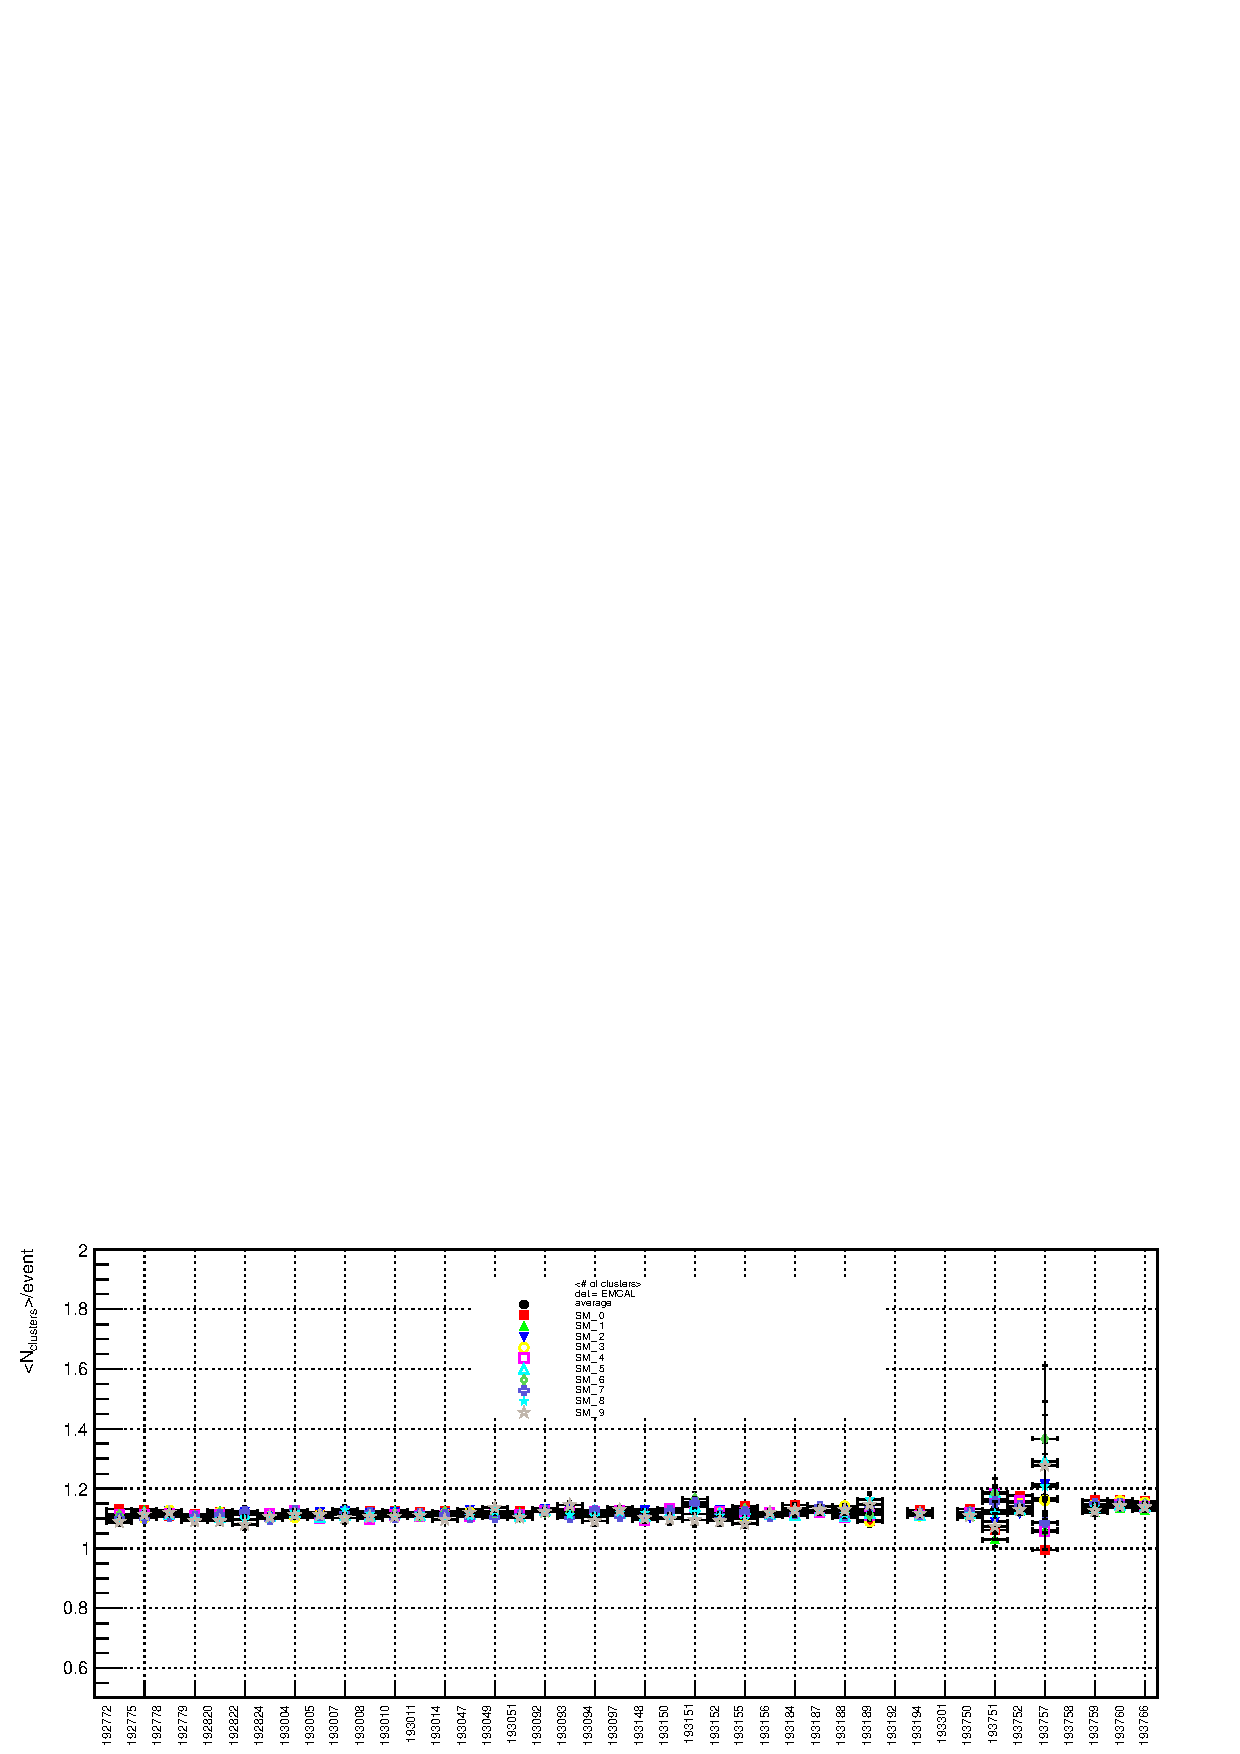
\includegraphics[width=0.9\textwidth]{figures/trendingClusterLHC12iMB.pdf}
\end{center}
\caption{\label{fig:trendingCluster}
Example of trending plot for period LHC12i: mean number of cluster per event as a function of runnumber for MinBias events.}
\end{figure}



{\bf $\pi^0$ Averages: (trendingPi0.C):}

This macro computes some fits over invariant mass histograms and store the fit parameters and $\pi^0$ computed values in a TGraph as a funcion of runnumber. The following histograms are used:
\begin{itemize}
\item EMCAL\_hIM: Invariant mass histogram filled over the whole cluster pairs.
\item EMCAL$\_$hIM$\_$Mod$\_$xx: Invariant mass histogram filled over the cluster pairs in the same supermodule.
\end{itemize}

The fit is  done by a gaussian plus  a 2$^{nd}$ order polinom for background. This is a very ``raw'' fitting wich may not be appropriate especially for the PbPb cases but allows to check the stabilities of averages (mass, width, number of $\pi^O$).



\begin{itemize}
\item Mean number of  $\pi^0$ per event is computed over EMCAL and also per supermodule.
\item Mass of the $\pi^0$ per event is computed over EMCAL and also per supermodule.
\item Witdh of the $\pi^0$ per event is computed over EMCAL and also per supermodule.
\end{itemize}



The use of these set of QA macros allows to identify problematic runs (subperiod with missing part of detectors) or more general features. Also it can be used to check global observables for different dataset used for analysis purpose. 



\subsection{Event display}

\subsection{Logbook tips}
\clearpage

\begin{thebibliography}{9}

\bibitem{EMCalTDR}
EMCal TDR
\url{http://aliceinfo.cern.ch/Documents/TDR/EMCAL.html}

\bibitem{DCalTDR}
DCal TDR
\url{https://cds.cern.ch/record/1272952/files/ALICE-TDR-014-ADD-1.pdf}

\bibitem{DCalGeoOff}
DCal Geometry implementation in offline
\url{https://indico.cern.ch/getFile.py/access?contribId=0&resId=0&materialId=slides&confId=229312}

\url{https://indico.cern.ch/event/229352/contribution/2/material/slides/0.pdf}

\bibitem{EMCAL:beginners} 
EMCal for beginners,
\url{ https://twiki.cern.ch/twiki/pub/ALICE/EMCalOffline/EMCalBeginners.pdf} 

\bibitem{ALIROOT}
AliRoot: ALICE offline project,
\url{http://aliceinfo.cern.ch/Offline/}

\bibitem{ALIROOT:doc} 
AliRoot Documentation,
 \url{ http://aliceinfo.cern.ch/Offline/AliRoot/Manual.html} 
 
 \bibitem{ALIROOT:install} 
AliRoot Installation,
\url{ http://aliceinfo.cern.ch/Offline/AliRoot/Installation.html} 

 \bibitem{ALIROOT:berzano} 
AliRoot Installation from Dario Berzano,
\url{ http://newton.ph.unito.it/~berzano/w/doku.php?id=alice:compile-any&redirect=1} 

\bibitem{EMCAL:MainTwiki} 
EMCal main twiki,
\url{ https://twiki.cern.ch/twiki/bin/viewauth/ALICE/EMCal} 

\bibitem{EMCAL:OffTwiki} 
EMCal Offline twiki,
\url{ https://twiki.cern.ch/twiki/pub/ALICE/EMCalOffline} 

 \bibitem{ALIEN:alien}
{AliEn web page},
 \url{ http://alien.cern.ch/twiki/bin/view/AliEn/Home}

\bibitem{ALIROOT:svn} 
AliRoot in GIT
\url{ http://git.cern.ch/pubweb/AliRoot.git/tree}

%\bibitem{EMCAL:doc} 
%EMCAL documentation,
%\url{ http://aliceinfo.cern.ch/Offline/Detectors/EMCALOffline.html} 

\bibitem{EMCAL:L0} 
EMCAL L0
\url{http://www.sciencedirect.com/science/article/pii/S0168900212007681#}

\bibitem{EMCAL:HLT} 
EMCAL HLT
\url{http://arxiv.org/abs/1209.3647}

\bibitem{EMCAL:TechDesignReport}
ALICE Collaboration, ALICE EMCal Technical Design Report, CERN/LHCC 2008-014

\bibitem{JetQuenchingIntro}
Casalderrey-Solana and C. A. Salgado, Introductory lectures on jet quenching in heavy ion collisions, Acta Phys. Polon. B 38 (2007) 3731

\bibitem{PPR1}
ALICE Collaboration, ALICE: Physics Performance Report, Volume I .J. Phys. G, 30 (2004) 1517-1763

\bibitem{PPR2}
ALICE Collaboration, ALICE: Physics Performance Report, Volume II. J. Phys. G, 32 (2006) 1295-2040

\bibitem{EMCALprepPEAK}
P. H. Hille, Fast Signal Extraction for the ALICE Electromagnetic Calorimeter, in preparation. 


\end{thebibliography}

\clearpage


\end{document}
